\documentclass{seuthesis-2022}

\title{基于领域自适应的}{工业过程故障诊断方法研究}
\author{陈鲲龙}
\studentnum{08022311}
\department{自动化学院}
\major{自动化}
\supervisor{王永健、童国道}
\period{2026年3月 \textasciitilde 2026年6月}
\SetKwInput{KwIn}{输入}
\SetKwInput{KwOut}{输出}
\SetKwFor{For}{循环}{执行}{结束循环}
\SetKwFor{ForEach}{遍历}{执行}{结束遍历}
\DontPrintSemicolon
\setlength{\emergencystretch}{2em}
\setlength{\textfloatsep}{10pt plus 2pt minus 2pt}
\setlength{\floatsep}{10pt plus 2pt minus 2pt}
\setlength{\intextsep}{10pt plus 2pt minus 2pt}
\renewcommand{\topfraction}{0.9}
\renewcommand{\bottomfraction}{0.8}
\renewcommand{\textfraction}{0.08}
\renewcommand{\floatpagefraction}{0.78}
\begin{document}
\hypersetup{
  pdfauthor={陈鲲龙},
  pdfcreator={seuthesis-2022}
}
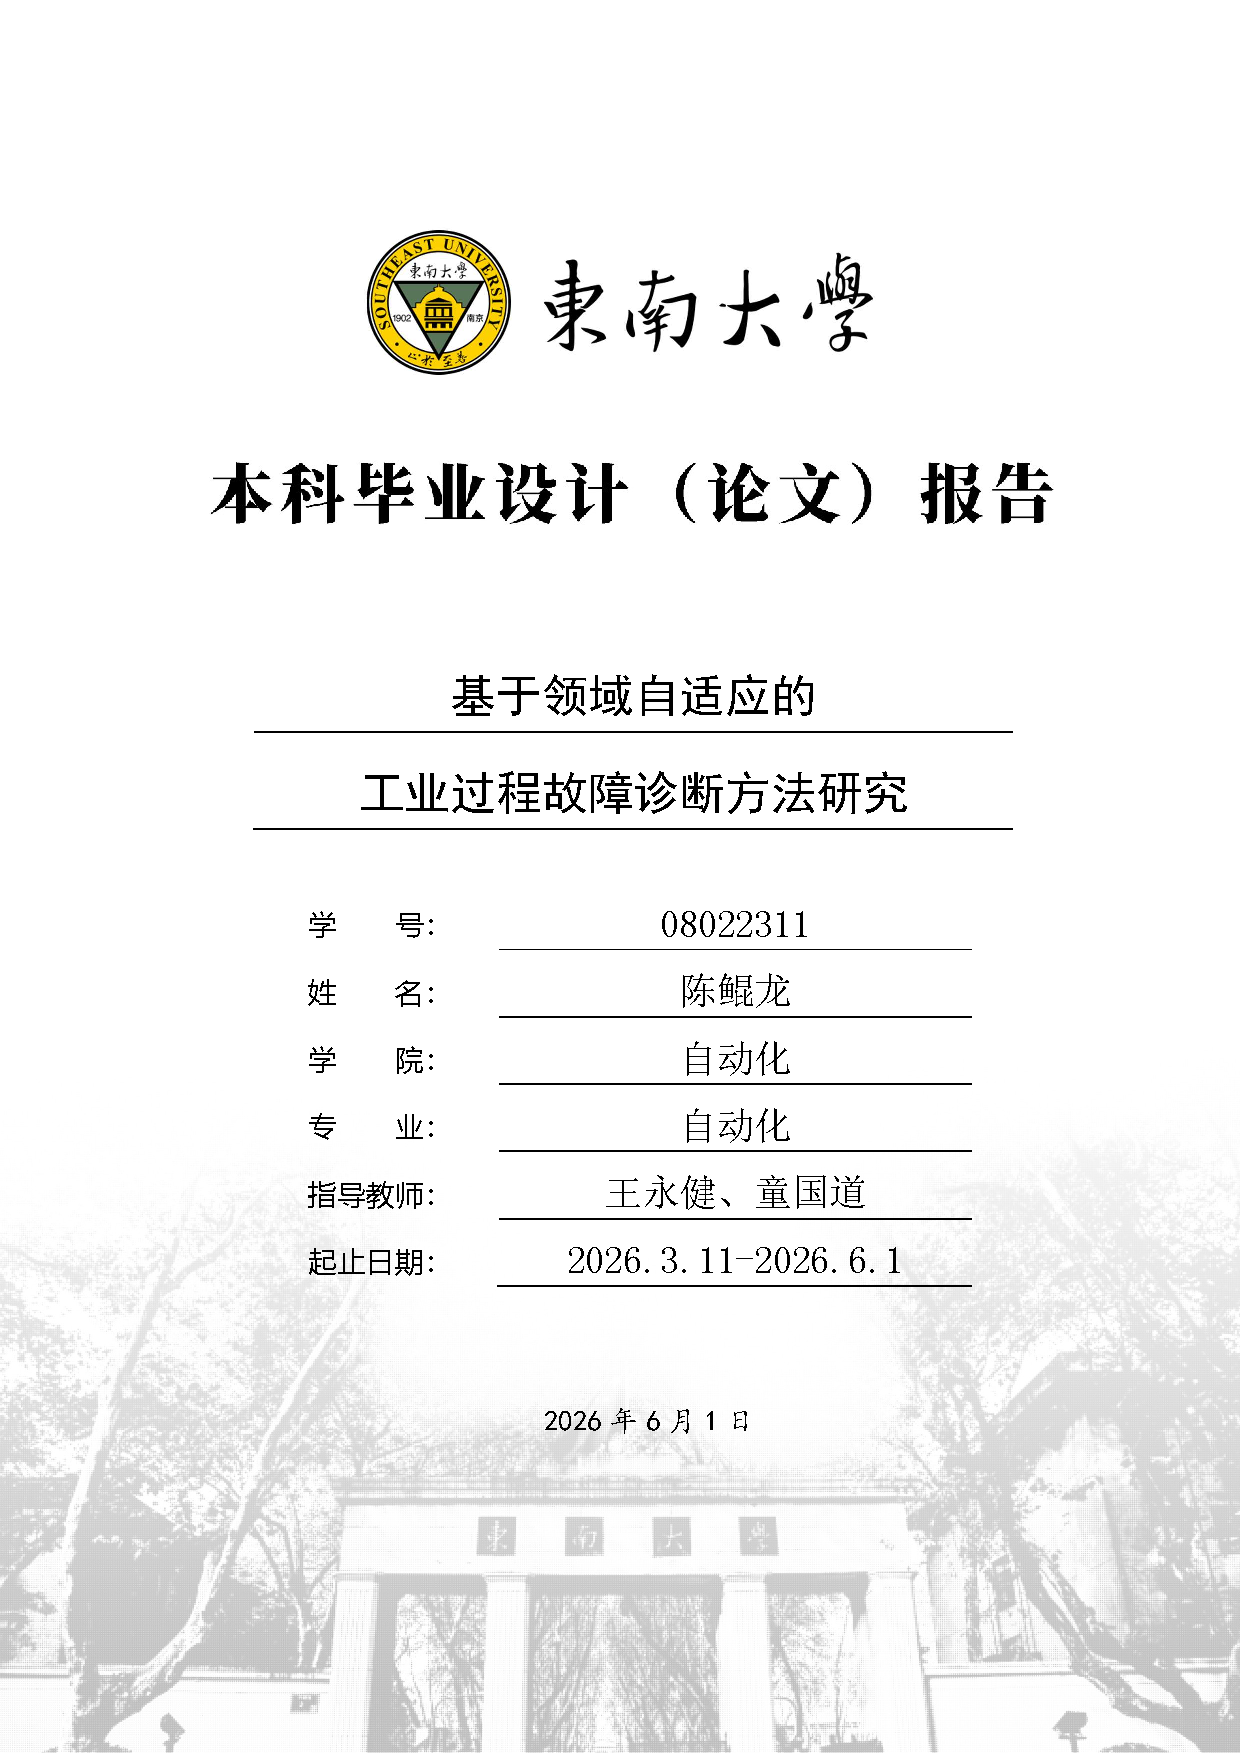
\includepdf[pages=1,pagecommand={\thispagestyle{empty}}]{resources/front_back_cover.pdf}
\makedeclaration
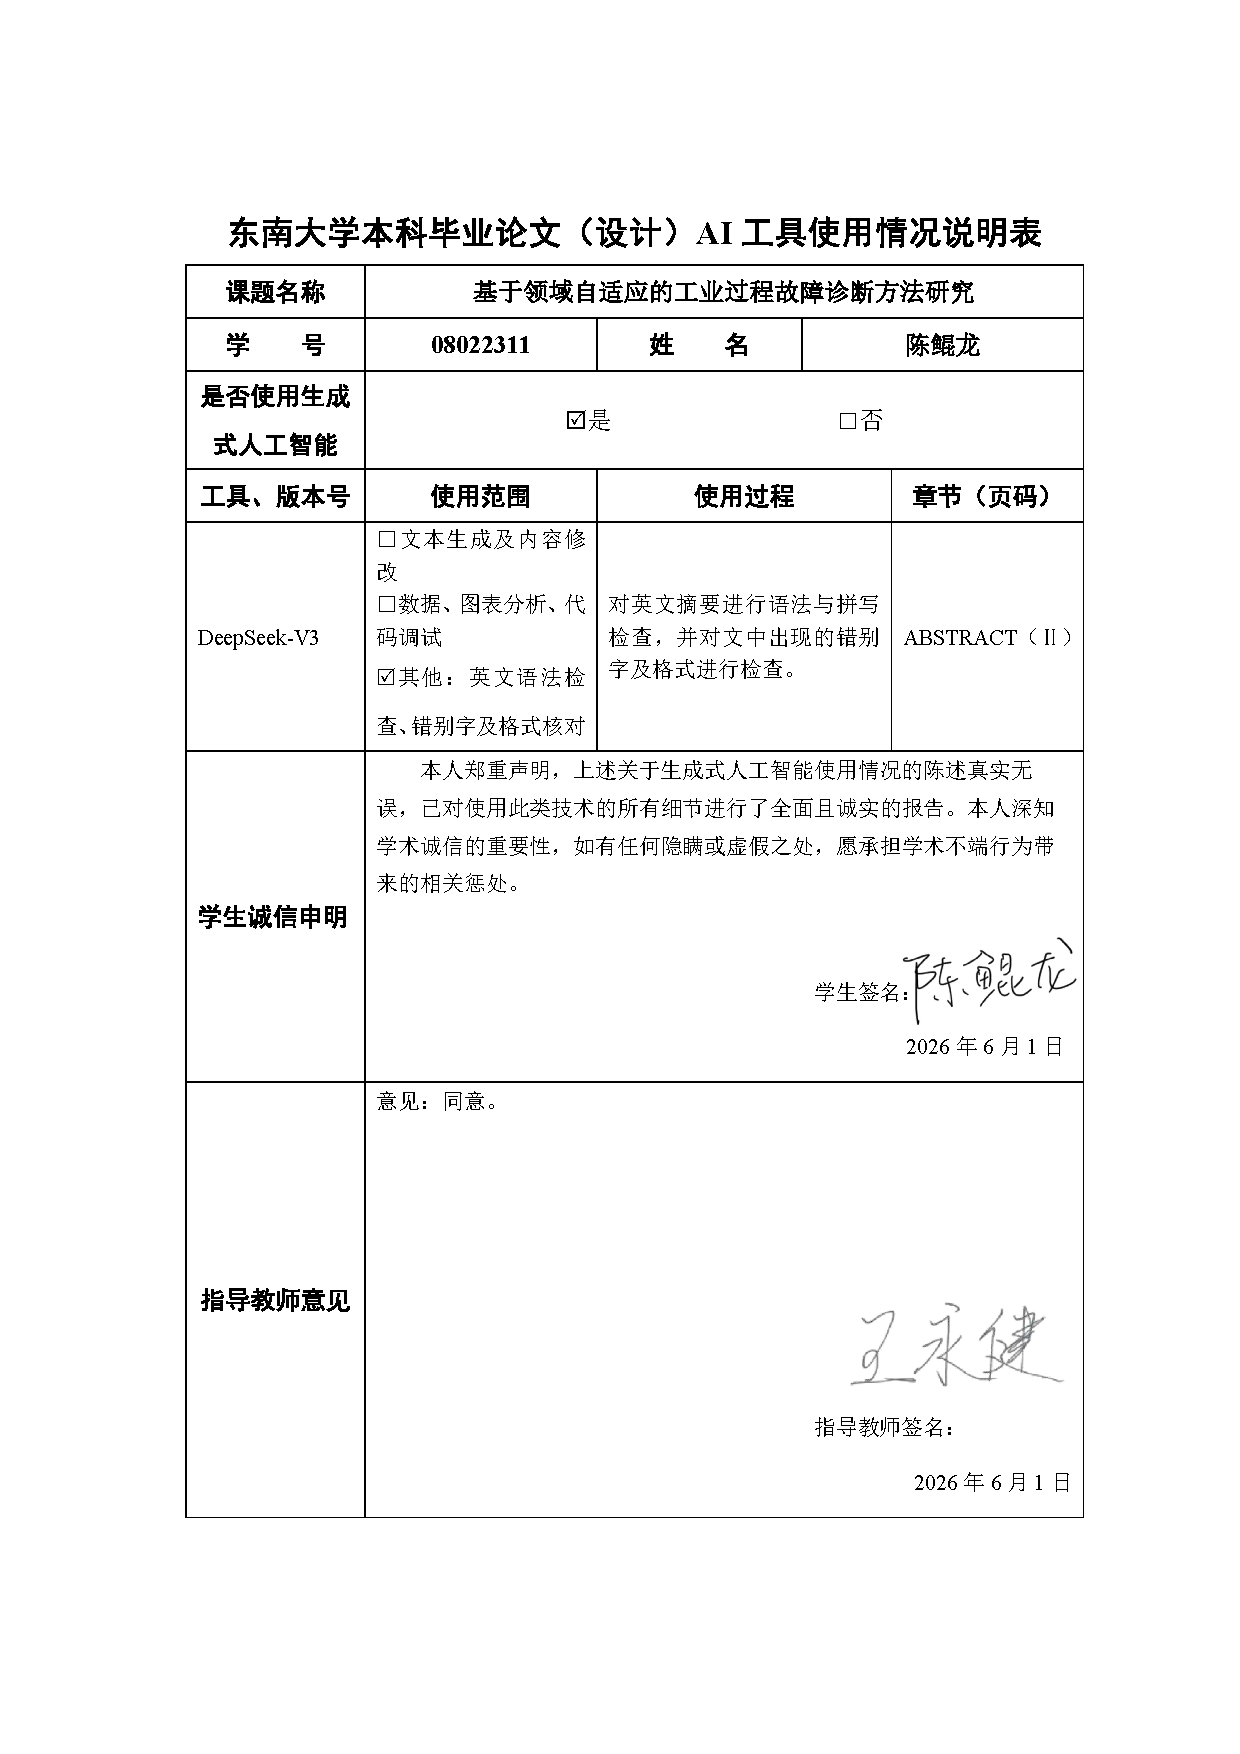
\includepdf[pages=-,pagecommand={\thispagestyle{empty}}]{resources/AI_used_claim.pdf}

\frontmatter
\begin{abstract}[zh]
工业过程故障诊断是过程监测与状态识别研究中的重要问题。跨工况诊断中，生产模式切换、工况变化、传感器统计特性变化和故障样本稀缺会引起源工况与目标工况之间的分布差异，使源工况训练得到的诊断模型难以直接泛化到目标工况。针对目标工况缺少标签条件下的跨工况诊断问题，本文以田纳西伊斯曼过程领域自适应数据集为研究对象，围绕单源域到单目标域和多源域到单目标域两类场景，研究基于领域自适应的工业过程故障诊断方法。

在单源场景中，本文以深度联合分布最优传输为基础，提出时序原型非平衡联合分布对齐方法。该方法通过非平衡传输减弱小批量训练中的错误强制匹配，并引入源域类别原型、时间序列统计代价和监督对比学习，以保持故障类别结构。针对目标域伪标签可靠性不足的问题，进一步提出多证据置信均衡伪标签方法，综合传输语义、教师预测语义和源域原型语义筛选目标样本，并利用动态阈值、类别均衡和强弱增强一致性约束提高无标签样本利用质量。在多源场景中，本文从原型距离、类条件传输代价、目标预测熵和源域类别性能等方面构建源域--故障类别可靠性矩阵，提出类条件源域可靠性加权方法，以支持更细粒度的多源选择性迁移。实验结果表明，所提方法能够提升跨工况故障诊断的目标域性能，并为分析不同源域和故障类别的迁移贡献提供依据。
\keywords{工业过程故障诊断,领域自适应,最优传输,伪标签学习,多源迁移}
\end{abstract}

\begin{abstract}[en]
Industrial process fault diagnosis is an important problem in process monitoring and condition recognition. In cross-condition diagnosis, changes in operating regimes, working conditions, sensor statistics, and the scarcity of labeled fault samples often lead to distribution shifts between source and target conditions. As a result, a diagnostic model trained under one operating condition may not generalize well to another. To address cross-condition diagnosis with limited or unavailable target labels, this thesis studies domain adaptation methods for industrial process fault diagnosis on the Tennessee Eastman process domain adaptation benchmark, considering both single-source to single-target and multi-source to single-target settings.

For the single-source setting, this thesis develops a temporal-prototype unbalanced joint distribution alignment method based on deep joint distribution optimal transport. Unbalanced transport is introduced to reduce unreliable forced matching in mini-batch alignment, while source-class prototypes, temporal statistical costs, and supervised contrastive learning are used to preserve fault-category structures. To further improve the use of unlabeled target samples, a confidence-balanced pseudo-labeling method is proposed. It combines transport semantics, teacher prediction semantics, and source-prototype semantics, and selects target samples using multi-evidence consistency, dynamic thresholds, class balancing, and weak-strong augmentation consistency. For the multi-source setting, this thesis proposes a class-conditional source reliability weighting method. A source-fault reliability matrix is constructed from prototype distance, class-conditional transport cost, target prediction entropy, and source-class performance, enabling fine-grained selective transfer across sources and fault categories. Experimental results show that the proposed methods improve target-domain diagnosis performance under cross-condition shifts and provide useful evidence for interpreting the contribution of different source domains and fault classes.
\keywords{\mbox{Industrial process fault diagnosis},\mbox{Domain adaptation},\mbox{Optimal transport},\newline \mbox{Pseudo-label learning},\mbox{Multi-source transfer}}
\end{abstract}

\tableofcontents

\mainmatter

\chapter{绪论}

\section{研究背景与意义}

工业过程通常具有多变量耦合、非线性动态和时变扰动等特征。石油化工、能源生产和流程制造等过程可由大量过程变量、控制变量和状态变量共同描述，故障状态会改变变量间相关结构和动态响应模式。因此，研究如何从过程观测数据中识别正常状态与故障类型，是过程监测、状态识别和可靠性分析中的重要问题。

工业过程故障诊断通常包括故障检测和故障识别两个环节。故障检测关注系统状态是否偏离正常分布，故障识别则进一步判断故障类型或故障来源。随着数据采集技术和计算方法的发展，基于数据驱动的故障诊断方法逐渐成为重要研究方向。相比依赖精确机理模型的传统方法，数据驱动方法能够从过程数据中学习故障特征，适用于复杂非线性系统和高维多变量过程。近年来，深度学习方法凭借端到端特征提取能力，在旋转机械、化工过程、能源系统和制造过程等故障诊断任务中表现出较强表征能力\cite{lei2020applications,wang2025comprehensive}。

然而，多数监督诊断模型依赖训练数据与测试数据独立同分布的假设。跨工况设定中，生产模式、负荷水平、环境扰动、传感器统计特性和控制策略变化均可能导致源域与目标域之间的分布偏移。当模型只在某一工况下训练并直接迁移到另一工况时，诊断性能通常会下降。与此同时，故障标签通常具有稀缺性，目标工况下的标注样本规模更加有限；若仅依赖监督学习范式，模型对目标域分布信息的利用不足。因此，如何利用源工况有标签数据，在目标工况少标签或无标签条件下提升诊断模型的泛化能力，是跨工况故障诊断研究需要解决的重要问题。

领域自适应是迁移学习中的重要研究方向，旨在利用源域有标签数据和目标域无标签数据，通过减小源域与目标域之间的分布差异，提高模型在目标域上的泛化能力\cite{pan2009survey,wang2025comprehensive}。在工业过程故障诊断中，不同生产模式、负载或环境条件可视为不同领域，而故障类别空间通常保持一致。因此，无监督领域自适应为跨工况故障诊断提供了合适的建模框架。借助该框架，模型能够在不依赖目标域标签的条件下利用目标域数据分布信息，从而缓解工况变化造成的性能退化。

本文选取田纳西伊斯曼过程领域自适应数据集作为研究对象。田纳西伊斯曼过程是化工过程控制与故障诊断领域广泛使用的仿真基准，其不同生产模式对应不同的数据分布。相关基准研究表明，不同生产模式下变量相关结构和 Wasserstein 距离存在差异，说明该数据集能够形成具有不同分布偏移程度的跨工况诊断任务\cite{montesuma2024benchmark}。本文围绕单源域到单目标域和多源域到单目标域两类场景，研究基于最优传输、时序原型、置信伪标签和类条件源域可靠性的领域自适应故障诊断方法，以分析目标工况标签缺失条件下的诊断泛化问题。

\section{国内外研究现状}

\subsection{工业过程故障诊断研究现状}

工业过程故障诊断方法大体可分为基于机理模型的方法、基于信号处理的方法和基于数据驱动的方法。过程监测综述研究表明，数据驱动建模已成为复杂流程工业监测与诊断的重要路线，其优势在于能够利用历史运行数据刻画多变量过程状态\cite{qin2012survey,ge2017review}。基于机理模型的方法依赖系统数学模型或先验知识，通过残差分析、状态估计和控制理论判断系统是否异常。这类方法可解释性较强，但在复杂工业过程中，精确建立机理模型往往十分困难，尤其是当系统具有强非线性、多变量耦合和复杂控制结构时，模型构建与参数辨识成本较高。

基于信号处理的方法通常通过时域、频域或时频域分析提取故障特征，再结合分类器进行故障识别。该类方法在旋转机械和传感器信号分析研究中较为常见，但其性能依赖人工特征设计，对不同设备和不同工况的适应能力有限。随着工业数据规模增大和计算能力提升，基于机器学习和深度学习的数据驱动方法逐渐成为故障诊断研究的主流方向。面向化工过程故障检测与诊断的综述进一步指出，支持向量机、随机森林、人工神经网络、卷积神经网络和循环神经网络等方法能够从历史数据中学习故障模式，并在多类故障诊断任务中表现出较高分类性能\cite{lei2020applications,taqvi2021review}。

在工业过程故障诊断中，过程数据通常表现为多变量时间序列。不同变量之间存在复杂相关关系，同一故障在不同时间阶段可能呈现不同动态响应。因此，如何从多变量时序数据中提取稳定、可判别的故障特征，是数据驱动诊断方法的关键。全卷积网络、长短期记忆网络、注意力机制和 Transformer 等结构已被用于时间序列故障诊断，以增强模型对局部趋势、长期依赖和变量间关系的建模能力。相关综述也指出，深度过程故障诊断仍面临跨工况泛化、类别不均衡、标注成本和可解释性等问题\cite{yu2023challenges}。

尽管深度学习方法在工业故障诊断中取得了显著进展，但多数方法仍依赖训练集与测试集独立同分布的假设。在跨工况设定中，设备状态、生产负荷、环境条件和控制设定的变化会导致数据分布偏移，使得模型在新工况下性能下降。此外，故障样本稀缺、类别不均衡和目标工况标注不足也限制了监督学习方法的适用范围。因此，如何在跨工况、少标签或无标签条件下提升诊断模型的泛化能力，成为当前工业过程故障诊断研究的重要方向。

\subsection{迁移学习研究现状}

迁移学习旨在利用已有任务或已有领域中的知识，提升目标任务或目标领域上的学习性能。当目标任务数据有限时，迁移学习能够缓解模型对大量标注数据的依赖。根据迁移对象不同，迁移学习可分为样本迁移、特征迁移、模型迁移和关系迁移等类型；根据源任务和目标任务是否一致，也可进一步区分为同构迁移、异构迁移、领域自适应和领域泛化等问题设置\cite{pan2009survey,li2022perspective}。

在故障诊断领域，迁移学习主要用于解决不同设备、不同负载、不同工况和不同数据采集条件之间的知识迁移问题。例如，在一个工况下采集的故障样本较为充分，而另一个工况下故障样本较少时，可以利用源工况模型或源工况特征辅助目标工况诊断。深度迁移学习进一步结合深度神经网络的表征学习能力和迁移学习的知识复用能力，使模型能够在跨工况诊断、跨设备诊断和小样本诊断中获得更强泛化性能\cite{li2022perspective}。

迁移学习在工业故障诊断中的应用主要有两类思路。第一类是预训练与微调，即先利用源域有标签数据训练特征提取器，再使用少量目标域有标签样本进行微调。这类方法形式较为直接，但需要目标域标签，在目标域完全无标签的场景下难以使用。第二类是特征对齐，即通过统计距离、对抗学习或最优传输等方法缩小源域与目标域特征分布差异，使源域训练得到的分类器能够迁移到目标域。相比监督微调，特征对齐更适合目标域标签缺失的场景。

然而，迁移学习并不总是带来正向效果。当源域与目标域差异较大，或者源域知识与目标域任务不匹配时，迁移可能导致目标域性能下降，即负迁移问题。在工业过程故障诊断中，不同工况之间的故障动态响应可能存在差异，同一故障类别在不同生产模式下的特征中心和变量相关结构也可能发生变化。因此，迁移学习方法不仅需要利用源域知识，还需要判断哪些知识适合迁移、何时进行迁移以及如何避免不可靠源域或不可靠样本对目标域造成干扰。

\subsection{领域自适应研究现状}

领域自适应是迁移学习中研究较为充分的一类问题。其典型设定为：源域拥有有标签样本，目标域只有无标签样本或少量标签样本，二者类别空间相同但数据分布不同。根据目标域标签使用情况，可分为有监督领域自适应、半监督领域自适应和无监督领域自适应。本文关注无监督领域自适应，即训练过程中不使用目标域标签，只利用源域标签和目标域无标签样本进行模型适配。

现有领域自适应方法可大致分为基于度量学习的方法、基于对抗学习的方法以及基于重构或生成的方法。基于度量学习的方法通过最小化源域与目标域之间的统计差异进行对齐，常用度量包括最大均值差异、相关对齐、条件分布差异和 Wasserstein 距离等。其中，最优传输方法能够在样本层面建立源域与目标域之间的匹配关系，并显式刻画从一个分布变换到另一个分布的最小代价，具有较强的几何解释性。DeepJDOT 将最优传输扩展到深度特征空间，通过联合考虑特征距离和标签预测代价，在对齐源目标分布的同时保留分类判别信息\cite{damodaran2018deepjdot}。

基于对抗学习的方法通常借助领域判别器，使特征提取器学习到难以区分源域和目标域的领域不变表示。领域对抗神经网络通过梯度反转层促使源目标特征混淆，条件对抗方法进一步将类别预测信息引入领域判别过程，以缓解纯边缘分布对齐可能造成的类别混淆。对于时间序列数据，CoDATS 提出卷积式时间序列领域自适应框架，利用时间序列卷积特征提取器和领域对抗学习完成跨域特征对齐，并支持多源数据利用\cite{wilson2020codats}。

在多源领域自适应场景中，模型可以利用多个源域的有标签数据适配同一个目标域。相比单源设置，多源数据提供了更丰富的运行模式和故障信息，但也带来了源域间分布差异和负迁移风险。若简单合并多个源域，模型可能忽略不同源域与目标域之间的差异，导致不可靠源域信息干扰目标域诊断。WJDOT 针对多源领域自适应问题，在最优传输框架下同时学习源目标分布对齐和源域权重，使模型能够利用源域多样性并降低不相关源域的影响\cite{turrisi2022wjdot}。

针对田纳西伊斯曼过程领域自适应数据集的基准研究表明，不同生产模式会引起明显的数据分布偏移，且基于最优传输的方法在该基准上整体优于部分基于最大均值差异和 H-distance 的方法\cite{montesuma2024benchmark}。该结论说明，最优传输方法适合刻画工业过程跨工况数据之间的几何分布差异。但与此同时，深度领域自适应方法可能因过度追求领域不变特征而削弱故障类别判别性，多源方法也可能因源域整体加权粒度过粗而难以处理类别级负迁移。因此，有必要在现有 DeepJDOT、WJDOT 和 CoDATS 等方法基础上，进一步引入故障时序结构、目标样本可靠性和类条件源域可靠性建模机制。

\section{国内外研究现状总结}

综合上述研究，工业过程故障诊断已由传统机理建模和人工特征设计逐步发展到深度学习与领域自适应阶段。深度学习方法能够自动提取多变量时序特征，提升复杂工业过程中的故障识别能力；迁移学习和领域自适应方法则用于缓解不同工况之间的数据分布偏移，为目标工况标签缺失条件下的故障诊断提供了可行思路。

现有方法在跨工况工业过程故障诊断中仍有改进空间。单源领域自适应方法多关注源域与目标域的整体分布对齐，对工业时间序列中的故障动态响应和类别结构利用不足。在最优传输框架中，若小批量样本内类别组成不匹配，平衡传输约束可能迫使目标样本与不可靠源样本匹配，造成错误对齐。目标域无标签条件下，伪标签质量也难以保证；若仅依据分类器置信度筛选目标样本，过置信错误预测和类别偏置可能放大伪标签噪声。对于多源领域自适应，不同源域对目标域的贡献并不一致，同一源域对不同故障类别的可迁移性也可能不同，仅使用源域整体权重难以刻画源域与故障类别之间的细粒度可靠性关系。此外，工业故障诊断模型还需要具备一定可解释性，以便分析源域、故障类别和迁移机制对目标域诊断结果的影响。

基于以上问题，本文围绕田纳西伊斯曼过程跨工况故障诊断任务，构建单源和多源两条领域自适应研究路线。单源路线以 DeepJDOT 为基础，依次引入时序原型非平衡联合分布对齐和多证据置信均衡伪标签学习；多源路线结合 CoDATS 的时间序列表征能力、WJDOT 的逐源联合分布传输思想以及类条件源域可靠性加权机制，提升多源场景下的选择性迁移能力。

\section{核心挑战与创新点}

本文的研究任务是在目标工况缺少标签的条件下，利用源工况有标签数据和目标工况无标签数据识别工业过程故障类型。结合田纳西伊斯曼过程数据特点和现有领域自适应方法的局限，本文主要关注以下三个问题。

第一，单源跨工况诊断中的类别结构保持问题。DeepJDOT 等联合分布最优传输方法能够在特征和标签预测联合空间中进行源目标对齐，但普通平衡传输在小批量训练中可能产生错误强制匹配，也缺少对工业时序故障动态结构和类别原型的显式建模。针对这一问题，本文提出时序原型非平衡联合分布对齐方法，在 DeepJDOT 基础上引入非平衡最优传输，降低不可靠样本被强制匹配的风险；同时构建源域类别原型和时间序列统计代价，并通过源域监督对比学习增强类内紧凑性和类间分离性，提高跨工况对齐过程中的故障类别结构保持能力。

第二，目标域无标签条件下的伪标签可靠性问题。目标域标签不可用时，模型通常需要借助伪标签利用目标域样本，但伪标签容易受到错误传输、过置信预测和类别偏置影响。对此，本文提出多证据置信均衡伪标签方法，从传输计划、教师模型预测和源域原型距离三个角度估计目标样本的语义分布。只有当多种证据一致且置信度满足要求时，目标样本才参与伪标签学习；同时引入动态置信阈值、类别均衡机制和强弱增强一致性约束，以降低错误伪标签传播和类别坍缩风险。

第三，多源跨工况诊断中的源域负迁移问题。多源场景能够提供更多有标签样本，但不同源域与目标域之间存在差异，简单合并源域或使用全局源域权重难以判断某一源域对具体故障类别是否可靠。针对该问题，本文提出类条件源域可靠性加权方法，将 CoDATS 的卷积式时间序列表征、WJDOT 的逐源联合分布最优传输和类条件源域可靠性矩阵结合起来，估计不同源域对不同故障类别的迁移贡献，并通过领域对抗特征约束与教师先验保护提高多源融合的稳定性。

综上，本文的主要创新点如下：

（1）提出基于时序原型非平衡联合分布对齐的单源领域自适应故障诊断方法。该方法利用非平衡最优传输缓解源目标样本错误强制匹配，并通过源域类别原型和时间序列统计代价增强故障结构表达，结合源域监督对比学习提高特征空间的类别可分性。

（2）提出基于多证据置信均衡伪标签的单源领域自适应故障诊断方法。该方法融合传输语义、教师预测语义和源域原型语义三类证据，对目标域样本进行一致性筛选，并结合动态置信阈值、类别均衡和强弱增强一致性约束，提高目标域无标签样本利用的可靠性。

（3）提出基于类条件源域可靠性加权的多源领域自适应故障诊断方法。该方法在多源场景下引入逐源联合分布最优传输和源域-故障类别可靠性矩阵，使模型能够根据不同源域对不同故障类别的贡献进行选择性迁移，从而缓解多源负迁移并提升多源诊断结果的可解释性。

\section{研究技术路线}

本文技术路线围绕“数据预处理—基础模型构建—单源方法改进—多源方法改进—实验验证与分析”展开。

在数据层面，本文整理田纳西伊斯曼过程领域自适应数据集。该数据集包含多个生产模式，每个生产模式对应一个领域；样本形式为多变量时间序列，标签包括正常状态和多类故障状态。针对不同变量尺度差异较大的特点，对各生产模式下的连续变量进行标准化处理，并按照固定实验划分构造训练和测试场景。实验中，目标域测试标签仅用于最终评价，不参与训练、参数确定或模型选择。

在模型层面，本文构建跨工况领域自适应故障诊断的基础框架。单源域到单目标域场景以 DeepJDOT 为基础，利用深度特征与标签预测的联合最优传输完成源目标对齐；多源域到单目标域场景以 WJDOT 为基础，通过逐源最优传输和源域权重学习建模多源迁移关系。考虑到工业过程数据具有多变量时间序列特征，本文引入卷积式时间序列特征提取结构和领域对抗约束，为多源场景提供时序表征基础。

围绕单源场景，本文提出两级递进改进。第一阶段针对 DeepJDOT 中平衡传输可能导致错误强制匹配以及故障类别结构保持不足的问题，提出时序原型非平衡联合分布对齐方法。第二阶段针对目标域伪标签不可靠问题，提出多证据置信均衡伪标签学习方法，从传输计划、教师模型和原型距离三个方面筛选可信目标样本，并引入类别均衡和一致性约束增强目标域学习稳定性。

围绕多源场景，本文提出类条件源域可靠性加权方法。该方法利用卷积式时间序列表征和领域对抗学习获得可迁移特征空间，再分别计算每个源域与目标域之间的联合分布最优传输代价，构建源域-故障类别可靠性矩阵。借助该矩阵，模型能够区分不同源域对不同故障类别的贡献，并结合教师先验保护机制完成多源诊断结果融合。

实验部分通过单源和多源跨工况任务验证所提方法。单源实验比较源域直接迁移、典型领域自适应方法、DeepJDOT 及本文单源改进方法；多源实验比较源域直接迁移、CoDATS、WJDOT 及本文多源改进方法。评价指标包括诊断准确率、宏平均 F1 值、平衡准确率、混淆矩阵和跨域特征可视化结果，并结合性能对比、典型场景分析和可解释性分析评价方法的有效性与适用范围。

\section{论文结构安排}

本文共分为七章，各章内容安排如下。

第一章为绪论。首先介绍工业过程故障诊断的研究背景与意义，分析跨工况故障诊断中分布偏移、目标域标签不足和多源负迁移等问题；然后综述工业过程故障诊断、迁移学习和领域自适应的研究现状；最后给出本文面临的核心挑战、主要创新点、研究技术路线和论文整体结构。

第二章为跨工况领域自适应故障诊断基本方法。该章介绍本文后续方法所依赖的基础理论和基础模型，包括基于联合分布最优传输的领域自适应方法、深度联合分布最优传输方法、多源加权联合分布最优传输方法，以及基于卷积式时间序列领域自适应的迁移诊断方法，为后续章节的方法设计提供理论基础。

第三章为基于时序原型非平衡联合分布对齐的单源领域自适应故障诊断方法。该章针对单源跨工况诊断中平衡最优传输可能导致错误匹配、故障类别结构表达不足等问题，提出结合非平衡最优传输、源域类别原型、时间序列统计代价和监督对比学习的单源领域自适应诊断模型。

第四章为基于多证据置信均衡伪标签的单源领域自适应故障诊断方法。该章在第三章方法基础上，进一步解决目标域伪标签不可靠问题。通过传输语义分布、教师预测语义分布和源域原型语义分布构造多证据伪标签，并结合动态置信阈值、类别均衡机制和强弱增强一致性约束，提高目标域样本利用的可靠性。

第五章为基于类条件源域可靠性加权的多源领域自适应故障诊断方法。该章面向多源跨工况诊断任务，提出结合卷积式时间序列表征、逐源联合分布最优传输和类条件源域可靠性矩阵的多源适配方法，从而支持对可靠源域和可靠故障类别的选择性迁移。

第六章为实验设计与结果分析。该章介绍田纳西伊斯曼过程领域自适应数据集、单源和多源实验场景、数据预处理方式、评价指标和对比方法，并通过准确率对比、混淆矩阵、特征可视化和源域可靠性分析本文方法的有效性。

第七章为总结与展望。该章总结全文主要研究内容和创新点，分析当前工作存在的不足，并对未来在弱监督目标域校准、在线测试时自适应、多源可解释迁移和轻量化建模等方向的研究进行展望。

\chapter{跨工况领域自适应故障诊断基本方法}

\section{引言}

工业过程故障诊断的目标是根据过程变量、控制变量和传感器信号判断系统是否发生故障，并进一步识别故障类别。在传统监督学习设置下，通常假设训练数据和测试数据服从相同或相近的概率分布。然而，在跨工况诊断设定中，生产模式切换、负荷变化、控制策略调整和环境扰动等因素都会导致数据分布偏移，使在源工况下训练得到的诊断模型难以直接泛化到目标工况。对于田纳西伊斯曼过程这类多模式化工过程，不同生产模式对应不同数据分布，而目标模式下的故障标签往往难以大量获取。因此，跨工况故障诊断可以建模为领域自适应问题。

无监督领域自适应的典型设置为：源域拥有有标签样本，目标域仅拥有无标签样本，源域与目标域共享相同的标签空间，但样本分布不同。设源域为
\begin{equation}
    \mathcal{D}_s=\{(x_i^s,y_i^s)\}_{i=1}^{n_s},
\end{equation}
目标域为
\begin{equation}
    \mathcal{D}_t=\{x_j^t\}_{j=1}^{n_t},
\end{equation}
其中 $x_i^s$ 和 $x_j^t$ 表示多变量时间序列样本，$y_i^s$ 表示源域故障类别标签。领域自适应的目标是在不使用目标域标签的条件下，学习一个诊断函数 $h$，使其在目标域样本上具有较高的分类准确率。由于源域和目标域之间存在分布差异，即
\begin{equation}
    P_s(X) \neq P_t(X),
\end{equation}
直接使用源域训练得到的模型往往会产生性能退化。

在现有领域自适应方法中，最优传输方法能够从分布几何角度度量源域和目标域之间的差异，并通过传输计划刻画样本之间的匹配关系\cite{courty2017otda}。与仅对齐均值或核空间统计量的方法相比，最优传输能够保留样本级匹配信息，因此适合处理跨工况工业过程数据中的复杂分布偏移。另一方面，对于多变量时间序列故障诊断任务，卷积式时间序列特征提取方法能够从原始序列中自动提取局部动态模式和全局故障表征\cite{wang2017time,fawaz2019deep}。基于领域对抗学习的特征对齐方法则通过领域判别器促使特征提取器学习源域和目标域难以区分的共享特征\cite{ganin2016dann}。

本章介绍后续方法所依赖的基础模型与理论。内容包括基于联合分布最优传输的领域自适应方法，其中涉及单源场景下的 DeepJDOT 和多源场景下的 WJDOT；同时介绍卷积式时间序列领域自适应方法，包括时间序列特征提取结构和基于领域对抗学习的特征对齐机制。这些内容为第三章、第四章和第五章的方法设计提供基础。

\section{基于联合分布最优传输的领域自适应方法}

最优传输是一类用于度量两个概率分布差异的数学工具。给定源分布和目标分布，最优传输通过寻找传输计划，使源分布中的质量搬运到目标分布所需的总代价最小。设源域样本集合为 $\{x_i^s\}_{i=1}^{n_s}$，目标域样本集合为 $\{x_j^t\}_{j=1}^{n_t}$，二者之间的代价矩阵为 $C \in \mathbb{R}^{n_s \times n_t}$，其中 $C_{ij}$ 表示源样本 $x_i^s$ 与目标样本 $x_j^t$ 之间的匹配代价。最优传输问题可写为
\begin{equation}
    \gamma^\ast
    =
    \arg\min_{\gamma \in \Pi(a,b)}
    \sum_{i=1}^{n_s}\sum_{j=1}^{n_t}
    \gamma_{ij} C_{ij},
\end{equation}
其中 $\gamma$ 为传输计划，$\Pi(a,b)$ 表示满足源域边际分布 $a$ 和目标域边际分布 $b$ 的传输计划集合，即
\begin{equation}
    \Pi(a,b)
    =
    \left\{
    \gamma \in \mathbb{R}_{+}^{n_s \times n_t}
    \mid
    \gamma \mathbf{1}_{n_t}=a,\,
    \gamma^{\mathrm{T}}\mathbf{1}_{n_s}=b
    \right\}.
\end{equation}
对于领域自适应任务而言，传输计划 $\gamma$ 不仅反映样本之间的距离关系，也可用于描述源域样本如何与目标域样本建立对应关系。

在故障诊断场景中，仅对齐特征分布并不一定能够保证类别判别性。如果源域某一类故障样本与目标域另一类故障样本在特征空间中被错误匹配，模型可能获得领域不变但类别混淆的特征表示。为缓解该问题，联合分布最优传输方法同时考虑特征空间距离和标签预测代价，使传输计划不仅关注源域和目标域样本在特征空间中的接近程度，也关注源域标签与目标域预测结果之间的一致性\cite{courty2017jdot}。

\subsection{深度联合分布最优传输方法}

深度联合分布最优传输方法（Deep Joint Distribution Optimal Transport，DeepJDOT）是面向单源无监督领域自适应的一类深度最优传输方法\cite{damodaran2018deepjdot}。该方法将深度神经网络分为特征提取器和分类器两部分。为与后文方法记号保持一致，设特征提取器为 $F_\theta(\cdot)$，分类器为 $G_\phi(\cdot)$，则输入样本 $x$ 的深度特征表示为
\begin{equation}
    z = F_\theta(x),
\end{equation}
对应的类别预测概率为
\begin{equation}
    \hat{y} = G_\phi(z).
\end{equation}

DeepJDOT 在深度特征和标签预测的联合空间中构造最优传输代价。对于源域样本 $(x_i^s,y_i^s)$ 和目标域样本 $x_j^t$，其联合传输代价通常由两部分组成：
\begin{equation}
    C_{ij}
    =
    \lambda_f \operatorname{dist}\left(F_\theta(x_i^s), F_\theta(x_j^t)\right)
    +
    \lambda_y \ell\left(y_i^s, G_\phi(F_\theta(x_j^t))\right),
\end{equation}
其中 $\operatorname{dist}(\cdot,\cdot)$ 表示特征空间距离，$\ell(\cdot,\cdot)$ 表示标签预测损失，$\lambda_f$ 和 $\lambda_y$ 分别为特征代价和标签代价的权重。第一项用于缩小源域与目标域在深度表征空间中的距离，第二项用于约束目标域样本的预测结果与其匹配的源域标签保持一致。

基于上述代价矩阵，DeepJDOT 的领域自适应损失可表示为
\begin{equation}
    \mathcal{L}_{\mathrm{OT}}
    =
    \sum_{i=1}^{n_s}\sum_{j=1}^{n_t}
    \gamma_{ij} C_{ij},
\end{equation}
其中 $\gamma_{ij}$ 表示源域样本 $i$ 与目标域样本 $j$ 之间的传输质量。模型训练时通常还需要保留源域监督分类损失：
\begin{equation}
    \mathcal{L}_{\mathrm{src}}
    =
    \frac{1}{n_s}
    \sum_{i=1}^{n_s}
    \ell\left(y_i^s,G_\phi(F_\theta(x_i^s))\right).
\end{equation}
因此，DeepJDOT 的总体优化目标可写为
\begin{equation}
    \min_{\theta,\phi}
    \mathcal{L}_{\mathrm{src}}
    +
    \lambda_{\mathrm{ot}}\mathcal{L}_{\mathrm{OT}},
\end{equation}
其中 $\lambda_{\mathrm{ot}}$ 为最优传输对齐损失的权重。

DeepJDOT 并非只对齐源域和目标域的边缘特征分布，而是在特征和标签预测组成的联合空间中进行对齐。该方式能够在减小领域差异的同时保留一定的类别判别信息，适用于源域有标签、目标域无标签的跨工况故障诊断任务。但在训练过程中，DeepJDOT 仍存在局限。普通最优传输通常采用平衡边际约束，要求源域和目标域样本质量均被完整匹配；在小批量训练中，若源域和目标域批次内类别组成不一致，目标样本可能被迫与不可靠源样本匹配。另一方面，DeepJDOT 的传输代价主要由深度特征距离和标签预测损失构成，尚未显式利用工业过程时间序列中的故障动态结构和类别原型信息。在目标域预测尚不可靠的训练早期，标签预测代价也可能受到错误预测影响，引入错误对齐。

因此，本文第三章在 DeepJDOT 的基础上进一步引入非平衡最优传输、源域类别原型、时间序列统计代价和源域监督对比学习，以增强单源跨工况故障诊断中的类别结构保持能力。

\subsection{多源加权联合分布最优传输方法}

在多源领域自适应场景中，模型可利用多个源域的有标签数据适配一个无标签目标域。设共有 $K$ 个源域，第 $k$ 个源域表示为
\begin{equation}
    \mathcal{D}_{s_k}
    =
    \{(x_i^{s_k},y_i^{s_k})\}_{i=1}^{n_k},
    \quad k=1,2,\cdots,K,
\end{equation}
目标域为
\begin{equation}
    \mathcal{D}_t=\{x_j^t\}_{j=1}^{n_t}.
\end{equation}
多源领域自适应不仅需要处理源域与目标域之间的分布偏移，还需要处理不同源域之间的分布差异，即
\begin{equation}
    P_{s_k}(X) \neq P_t(X),
    \quad
    P_{s_k}(X) \neq P_{s_l}(X),
    \quad k \neq l.
\end{equation}

一种简单策略是将所有源域样本合并为一个大源域，再执行单源领域自适应。然而，该策略容易忽略不同源域之间的差异。当某些源域与目标域差异较大时，这些源域中的信息可能对目标域诊断造成干扰，引发负迁移。多源加权联合分布最优传输方法（Weighted Joint Distribution Optimal Transport，WJDOT）通过为不同源域分配权重，在利用多源数据的同时降低不可靠源域的影响\cite{turrisi2022wjdot}。

对于第 $k$ 个源域，可构造其与目标域之间的联合传输代价：
\begin{equation}
    C_{ij}^{(k)}
    =
    \lambda_f \operatorname{dist}\left(F_\theta(x_i^{s_k}),F_\theta(x_j^t)\right)
    +
    \lambda_y \ell\left(y_i^{s_k},G_\phi(F_\theta(x_j^t))\right).
\end{equation}
对应的最优传输损失为
\begin{equation}
    \mathcal{L}_{\mathrm{OT}}^{(k)}
    =
    \sum_{i=1}^{n_k}\sum_{j=1}^{n_t}
    \gamma_{ij}^{(k)} C_{ij}^{(k)}.
\end{equation}
WJDOT 进一步引入源域权重 $\alpha_k$，使不同源域对最终目标函数的贡献不同：
\begin{equation}
    \mathcal{L}_{\mathrm{WJDOT}}
    =
    \sum_{k=1}^{K}
    \alpha_k
    \mathcal{L}_{\mathrm{OT}}^{(k)},
    \quad
    \sum_{k=1}^{K}\alpha_k=1,
    \quad
    \alpha_k \geq 0.
\end{equation}
其中，$\alpha_k$ 越大，表示第 $k$ 个源域对目标域适配越重要；$\alpha_k$ 越小，表示该源域可能与目标域差异较大或对目标域贡献较弱。

WJDOT 的特点在于保留多源域差异，并通过源域重加权机制利用有益源域、抑制不可靠源域。对于田纳西伊斯曼过程这类多生产模式数据，不同模式之间存在不同程度的相似性，部分源模式对某一目标模式具有较好迁移效果，而另一些源模式可能引入负迁移。因此，多源加权思想适合用于跨工况故障诊断。

不过，WJDOT 的源域权重通常作用于整个源域，无法直接刻画“某个源域对某个故障类别是否可靠”。在工业过程故障诊断中，一个源域整体上接近目标域，并不意味着它对所有故障类别都具有相同可迁移性。例如，某一生产模式可能对正常类和部分故障类具有较好迁移能力，但对其他故障类存在明显偏移。因此，本文第五章将在 WJDOT 基础上引入类条件源域可靠性矩阵，将源域整体加权扩展为源域--故障类别级别的可靠性加权。

\section{基于卷积式时间序列领域自适应的迁移诊断方法}

工业过程数据通常表现为多变量时间序列。相比图像数据或普通表格数据，时间序列数据具有时间相关性、动态变化性和变量耦合性等特点。对于田纳西伊斯曼过程，每个样本由多个连续变量在一段时间内的采样值组成，不同故障会在时间维度上表现出不同动态响应模式。因此，在跨工况故障诊断中，特征提取器不仅需要提取每个变量的局部变化，还需要捕捉不同时间段和不同变量之间的综合故障信息。

CoDATS 是一种面向时间序列传感器数据的卷积式深度领域自适应方法，通过卷积式时间序列特征提取器学习可迁移表征，并结合领域对抗学习减小源域与目标域之间的特征分布差异\cite{wilson2020codats}。与直接使用通用图像领域自适应网络不同，CoDATS 针对时间序列数据设计特征提取结构，因此适合作为本文多源跨工况实验中的对比基线和表征基础。

\subsection{卷积式时间序列特征提取方法}

卷积神经网络能够通过局部卷积核提取时间序列中的局部动态模式。在多变量时间序列故障诊断中，输入样本可表示为
\begin{equation}
    x \in \mathbb{R}^{V \times L},
\end{equation}
其中 $V$ 表示变量或通道数，$L$ 表示时间窗口长度。对于田纳西伊斯曼过程数据，$V$ 对应连续过程变量数量，$L$ 对应一个样本窗口内的采样时间长度。

一维卷积层通过在时间维度上滑动卷积核提取局部时间特征。设第 $l$ 层输入为 $U^{(l-1)}$，卷积核参数为 $W^{(l)}$，偏置为 $b^{(l)}$，则卷积输出可表示为
\begin{equation}
    U^{(l)}
    =
    \varphi\left(W^{(l)} * U^{(l-1)} + b^{(l)}\right),
\end{equation}
其中 $*$ 表示卷积运算，$\varphi(\cdot)$ 表示非线性激活函数。通过堆叠多层卷积网络，模型能够从短期局部波动逐渐学习到更高层次的故障模式。

在时间序列分类任务中，全卷积网络常由多个一维卷积块和全局平均池化层组成\cite{wang2017time,fawaz2019deep}。卷积块用于提取局部动态特征，归一化层用于稳定训练过程，非线性激活函数用于增强模型表达能力，全局平均池化层用于将时间维度特征压缩为固定长度向量。设最后一层卷积输出为 $U \in \mathbb{R}^{d_z \times L'}$，全局平均池化可表示为
\begin{equation}
    z_r
    =
    \frac{1}{L'}
    \sum_{t=1}^{L'}
    U_{r,t},
    \quad r=1,2,\cdots,d_z,
\end{equation}
其中 $z$ 为最终时间序列特征表示。

卷积式时间序列特征提取方法适合处理多变量过程数据。卷积核能够捕捉故障发生后过程变量在局部时间范围内的变化趋势，多层卷积结构可以逐步扩大感受野，从而学习较长时间范围内的动态响应。全局平均池化能够减少模型参数数量，降低过拟合风险；相比循环神经网络，卷积结构训练效率较高，也更适合大规模多变量时间序列实验。

在本文中，卷积式时间序列特征提取器不仅用于对比方法 CoDATS，也为第五章的多源改良方法提供基础表征。由于最优传输代价依赖样本在特征空间中的距离，特征提取器的质量会直接影响传输计划的可靠性。若特征表示无法区分故障类别，即使后续采用最优传输或源域加权机制，也难以获得理想适配效果。因此，利用卷积式时间序列网络构建稳定的故障表征，是多源跨工况故障诊断的重要基础。

\subsection{基于领域对抗学习的特征对齐方法}

领域对抗学习是一类典型的深度领域自适应方法。该方法利用领域判别器判断特征来自源域还是目标域，并训练特征提取器生成使领域判别器难以区分的特征表示。通过这种对抗训练，特征提取器在保持源域分类能力的同时，可以学习源域和目标域共享的领域不变特征\cite{ganin2016dann}。

设特征提取器为 $F_\theta(\cdot)$，故障分类器为 $G_\phi(\cdot)$，领域判别器为 $D_\omega(\cdot)$。对于源域样本，分类器根据特征输出故障类别预测；对于源域和目标域样本，领域判别器输出其所属领域。源域分类损失为
\begin{equation}
    \mathcal{L}_{\mathrm{src}}
    =
    -\frac{1}{n_s}
    \sum_{i=1}^{n_s}
    \sum_{c=1}^{N_c}
    \mathbb{I}(y_i^s=c)
    \log G_{\phi,c}(F_\theta(x_i^s)),
\end{equation}
其中 $N_c$ 为故障类别数，$G_{\phi,c}(\cdot)$ 表示分类器输出属于第 $c$ 类的概率。

领域判别损失可表示为
\begin{equation}
    \mathcal{L}_{\mathrm{dom}}
    =
    -\frac{1}{n_s}
    \sum_{i=1}^{n_s}
    \log D_\omega(F_\theta(x_i^s))
    -
    \frac{1}{n_t}
    \sum_{j=1}^{n_t}
    \log \left(1-D_\omega(F_\theta(x_j^t))\right).
\end{equation}
领域判别器希望最小化 $\mathcal{L}_{\mathrm{dom}}$，从而正确区分源域和目标域；特征提取器则希望最大化该损失，使源域和目标域特征变得难以区分。该对抗过程可写为
\begin{equation}
    \min_{F_\theta,G_\phi}
    \max_{D_\omega}
    \mathcal{L}_{\mathrm{src}}
    -
    \lambda_d \mathcal{L}_{\mathrm{dom}},
\end{equation}
其中 $\lambda_d$ 为领域对抗损失权重。领域对抗学习通常借助梯度反转思想，使领域判别器倾向于区分源域和目标域，而特征提取器倾向于学习使二者难以区分的共享表示。

CoDATS 将卷积式时间序列特征提取结构与领域对抗学习相结合，用于时间序列传感器数据的领域自适应。对于多源场景，CoDATS 可利用多个源域的有标签数据训练分类器，并通过领域对抗约束缩小源域和目标域之间的特征差异。其优势在于能够直接面向时间序列数据学习较强的深度表征，并通过对抗训练增强跨域泛化能力。

不过，领域对抗学习也存在一定局限。该方法主要强调源域和目标域整体特征分布难以区分，但并不能保证同一故障类别在不同领域之间正确对齐。若过度追求领域不变性，可能削弱类别判别信息，导致故障类别边界模糊。在多源场景中，不同源域对目标域的贡献并不一致，若领域对抗学习简单合并所有源域，则难以区分有益源域和不可靠源域。此外，领域判别器提供的是整体领域混淆信号，缺少对具体源域和具体故障类别迁移贡献的解释。

因此，本文第五章以 CoDATS 的卷积式时间序列表征和领域对抗约束作为多源方法基础，并利用 WJDOT 的逐源联合分布最优传输和类条件源域可靠性加权机制刻画源域与故障类别之间的细粒度迁移关系。通过结合时间序列表征、最优传输对齐和类条件源域可靠性建模，多源跨工况故障诊断可以同时考虑表征能力、迁移性能和解释性。

\section{本章小结}

本章介绍了跨工况领域自适应故障诊断所需的基本方法。针对源域有标签、目标域无标签的跨工况诊断问题，首先说明了基于联合分布最优传输的领域自适应思想。DeepJDOT 通过在深度特征和标签预测联合空间中构造最优传输代价，完成单源域与目标域之间的对齐；WJDOT 则进一步引入源域权重，使模型在多源场景下能够利用可靠源域并抑制不可靠源域。

本章还介绍了卷积式时间序列领域自适应方法。卷积式时间序列特征提取结构能够从多变量过程数据中学习局部动态模式和全局故障表示；基于领域对抗学习的特征对齐方法通过领域判别器与特征提取器之间的对抗优化，促使模型学习源域和目标域共享的领域不变特征。CoDATS 将时间序列卷积特征提取与领域对抗学习结合，适合处理多源时间序列传感器数据的跨域迁移诊断任务。

总体来看，DeepJDOT 为第三章和第四章的单源领域自适应方法提供联合分布最优传输基础，WJDOT 为第五章的多源加权迁移提供源域重加权基础，CoDATS 则为多源跨工况故障诊断提供时间序列表征和领域对抗对齐基础。现有方法仍存在平衡传输可能错误匹配、故障类别结构建模不足、目标伪标签可靠性不足以及多源源域权重粒度较粗等问题。后续章节将在上述基础上分别提出时序原型非平衡联合分布对齐方法、多证据置信均衡伪标签方法和类条件源域可靠性加权方法。

\chapter[基于时序原型非平衡联合分布对齐的单源领域自适应故障诊断方法]{基于时序原型非平衡联合分布对齐的\\单源领域自适应故障诊断方法}
\section{引言}

第二章介绍了 DeepJDOT 的基本做法：在深度特征与标签预测的联合空间中构造最优传输代价，使源域有标签样本与目标域无标签样本建立样本级匹配关系。该方法继承了联合分布最优传输在类别保持方面的优势\cite{courty2017jdot,damodaran2018deepjdot}，但用于工业过程跨工况故障诊断时仍存在两个问题。

一方面，田纳西伊斯曼过程样本为多变量时间序列，不同生产模式下同一故障类别的均值漂移、波动幅度和动态变化趋势可能同时发生改变。若仅使用深度特征距离和分类预测代价构造传输矩阵，模型容易忽略原始时序统计结构。另一方面，小批量训练时源域和目标域批次的类别组成并不总是匹配。普通平衡最优传输要求源域和目标域边际质量被完整匹配，当批次内某些类别缺失或目标样本暂时无法可靠匹配时，平衡约束可能迫使样本与错误类别发生传输，造成错误对齐。

针对上述问题，本章提出时序原型非平衡联合分布对齐方法。该方法在 DeepJDOT 基础上引入非平衡小批量最优传输，使部分不可靠传输质量可以被削减；同时维护源域类别原型，并利用目标样本到源域类别原型的相对距离修正传输代价；此外，从原始过程窗口中提取均值、标准差和一阶差分统计量，构造时间序列统计代价。训练前期还使用源域监督对比学习增强特征空间的类内紧凑性和类间分离性。本章方法训练过程中不使用目标域标签，目标域标签只在最终实验评价阶段使用。方法整体结构如图 \ref{fig:ch3_tpu_architecture} 所示。

\begin{figure}[!htbp]
    \centering
    \resizebox{\textwidth}{!}{\begin{tikzpicture}[
    x=1cm,
    y=1.35cm,
    >=stealth,
    font=\small\fontspec{Times New Roman}\songti,
    card/.style={
        draw,
        rounded corners=4pt,
        line width=0.45pt,
        fill=white
    },
    chip/.style={
        draw,
        rounded corners=2pt,
        line width=0.35pt,
        fill=white,
        align=center,
        inner xsep=5pt,
        inner ysep=5pt
    },
    bluecard/.style={card, draw=blue!45!black, fill=blue!4},
    cyancard/.style={card, draw=cyan!50!black, fill=cyan!5},
    orangecard/.style={card, draw=orange!65!black, fill=orange!6},
    greencard/.style={card, draw=green!45!black, fill=green!6},
    redcard/.style={card, draw=red!45!black, fill=red!5},
    panel/.style={draw=black!15, rounded corners=5pt, line width=0.35pt, fill=gray!1},
    arrow/.style={->, line width=0.55pt, draw=black!70},
    note/.style={font=\scriptsize\fontspec{Times New Roman}\songti, align=center}
]

\draw[panel] (-0.25,0.00) rectangle (17.95,9.00);
\node[font=\large\fontspec{Times New Roman}\songti] at (8.85,8.55)
    {TPU-DeepJDOT 时序原型非平衡联合分布对齐机制};

% 输入批次
\draw[bluecard] (0.55,2.15) rectangle (3.25,7.75);
\node at (1.90,7.43) {输入批次};
\node[chip, minimum width=2.05cm] at (1.90,6.05)
    {源域有标签\\[-1pt]$\mathcal{B}_s$};
\node[chip, minimum width=2.05cm] at (1.90,4.60)
    {目标域无标签\\[-1pt]$\mathcal{B}_t$};
\node[note, text width=2.20cm] at (1.90,3.25)
    {训练阶段不使用目标标签};

% 时序诊断网络
\draw[cyancard] (4.05,2.15) rectangle (7.55,7.75);
\node at (5.80,7.43) {时序诊断网络};
\node[chip, minimum width=2.60cm] at (5.80,6.05)
    {共享 FCN 表征\\[-1pt]$z=F_\theta(x)$};
\node[chip, minimum width=2.60cm] at (5.80,4.60)
    {诊断分类器\\[-1pt]$p=G_\phi(z)$};
\node[note, text width=2.75cm] at (5.80,3.25)
    {源域监督形成基础判别边界};

% 结构增强约束
\draw[orangecard] (8.35,2.15) rectangle (11.95,7.75);
\node at (10.15,7.43) {结构增强约束};
\node[chip, minimum width=2.75cm] at (10.15,6.25)
    {源域类别原型\\[-1pt]$\mu_c,\ r_{ij}^{\mathrm{proto}}$};
\node[chip, minimum width=2.75cm] at (10.15,4.95)
    {时序统计描述符\\[-1pt]$\psi(x),\ c_{ij}^{\mathrm{temp}}$};
\node[chip, minimum width=2.75cm] at (10.15,3.65)
    {源域监督对比\\[-1pt]$\mathcal{L}_{\mathrm{supcon}}$};
\node[note, text width=2.90cm] at (10.15,2.60)
    {修正传输代价，预热源类结构};

% 非平衡联合传输
\draw[greencard] (12.75,2.15) rectangle (17.25,7.75);
\node at (15.00,7.43) {非平衡联合传输};
\node[chip, minimum width=3.35cm] at (15.00,6.25)
    {联合代价矩阵\\[-1pt]$C_{ij}$};
\node[chip, minimum width=3.35cm] at (15.00,4.95)
    {非平衡 Sinkhorn\\[-1pt]$\gamma^\ast,\tau_s,\tau_t$};
\node[chip, minimum width=3.35cm] at (15.00,3.65)
    {对齐损失\\[-1pt]$\mathcal{L}_{\mathrm{align}}$};
\node[note, text width=3.35cm] at (15.00,2.60)
    {边际质量可削减，缓解错误强制匹配};

% 优化目标
\draw[redcard] (4.05,0.50) rectangle (17.25,1.35);
\node at (10.65,0.92)
    {$\mathcal{L}_{\mathrm{TPU}}
    =\mathcal{L}_{\mathrm{src}}
    +\lambda_{\mathrm{supcon}}\mathcal{L}_{\mathrm{supcon}}
    +\lambda_{\mathrm{ot}}\mathcal{L}_{\mathrm{align}}$};

\draw[arrow] (3.25,4.95) -- (4.05,4.95);
\draw[arrow] (7.55,4.95) -- (8.35,4.95);
\draw[arrow] (11.95,4.95) -- (12.75,4.95);
\draw[arrow] (15.00,2.15) -- (15.00,1.35);

\end{tikzpicture}
}
    \caption{时序原型非平衡联合分布对齐方法架构示意}
    \label{fig:ch3_tpu_architecture}
\end{figure}

\section{时序原型非平衡联合分布对齐基本原理}

设源域样本为 $\mathcal{D}_s=\{(x_i^s,y_i^s)\}_{i=1}^{n_s}$，目标域无标签样本为 $\mathcal{D}_t=\{x_j^t\}_{j=1}^{n_t}$。其中，$x\in\mathbb{R}^{V\times L}$ 表示包含 $V$ 个过程变量和 $L$ 个时间步的多变量时间序列窗口，$y_i^s\in\{1,2,\cdots,N_c\}$ 为源域故障类别标签。模型由时间序列特征提取器 $F_\theta$ 和分类器 $G_\phi$ 组成：
\begin{equation}
    z = F_\theta(x), \quad
    p = G_\phi(z).
\end{equation}
其中 $z$ 为深度特征表示，$p$ 为类别预测概率。

本文采用一维全卷积网络作为特征提取器。其结构包括核大小为 $9$、$5$、$3$ 的三层一维卷积块，每个卷积块后接归一化和 ReLU 激活，最后在时间维度上进行全局平均池化，得到固定维度的样本表示。全卷积网络是时间序列分类中常用且表现稳定的基线结构\cite{wang2017time,fawaz2019deep}，适合在 TEP 多变量时间序列上提取局部动态响应和全局故障表征。

\subsection{非平衡最优传输对齐原理}

最优传输从分布几何角度度量两个经验分布之间的差异，是领域自适应中刻画源目标分布偏移的重要工具\cite{peyre2019computational,courty2017otda}。给定源域小批量特征 $\{z_i^s\}_{i=1}^{n_s^{\mathrm{bat}}}$ 和目标域小批量特征 $\{z_j^t\}_{j=1}^{n_t^{\mathrm{bat}}}$，传统平衡最优传输要求传输计划 $\gamma$ 同时满足固定源边际和目标边际：
\begin{equation}
    \gamma\mathbf{1}_{n_t^{\mathrm{bat}}}=a,\quad
    \gamma^{\mathrm T}\mathbf{1}_{n_s^{\mathrm{bat}}}=b.
\end{equation}
在小批量领域自适应中，该约束可能过强。若当前小批量中源域某些类别样本过多，而目标域对应类别样本不足，平衡约束会要求所有源域质量被完整分配，进而可能产生错误匹配。

非平衡最优传输通过放松边际约束缓解该问题。受非平衡小批量最优传输领域自适应思想启发\cite{fatras2021unbalanced}，本文在传输目标中加入边际偏离惩罚：
\begin{equation}
    \mathcal{L}_{\mathrm{UOT}}
    =
    \min_{\gamma\geq 0}
    \langle \gamma, C\rangle
    +
    \varepsilon \mathrm{KL}(\gamma\|ab^{\mathrm T})
    +
    \tau_s \mathrm{KL}(\gamma\mathbf{1}_{n_t^{\mathrm{bat}}}\|a)
    +
    \tau_t \mathrm{KL}(\gamma^{\mathrm T}\mathbf{1}_{n_s^{\mathrm{bat}}}\|b),
\end{equation}
其中 $C$ 为联合传输代价矩阵，$\varepsilon$ 为熵正则系数，$\tau_s$ 和 $\tau_t$ 分别控制源边际与目标边际的放松程度。$\tau_s$、$\tau_t$ 越大，传输计划越接近平衡传输；二者较小时，部分不可靠质量可以被削减。小批量传输计划可通过非平衡 Sinkhorn 形式求解，传输质量、边际偏差和传输熵等量可用于分析源目标匹配状态。

在本文方法中，非平衡传输并不改变无监督领域自适应的基本设定。目标域标签不参与传输计划求解，传输计划只由源域标签、源目标特征、目标预测分布、源域原型和时序统计代价共同决定。

\subsection{源域类别原型约束原理}

类别原型通过类内样本特征均值表示类别中心，是度量学习和小样本学习中的常用思想\cite{snell2017prototypical}。在领域自适应中，原型结构也常用于缓解伪标签噪声和维护目标域语义结构\cite{zhang2021proda}。本文并不直接使用目标标签构造目标原型，而是在训练过程中维护源域类别原型，并利用源域类别结构约束目标样本的传输匹配。

设第 $c$ 类源域原型为 $\mu_c$。对于一个源域小批量，先对源域特征进行归一化，再按源标签求类均值：
\begin{equation}
    \bar{\mu}_c
    =
    \frac{1}{|\mathcal{B}_s^c|}
    \sum_{i:y_i^s=c}
    \frac{z_i^s}{\|z_i^s\|_2}.
\end{equation}
为降低小批量波动，本文采用指数滑动平均更新源域原型：
\begin{equation}
    \mu_c
    \leftarrow
    \frac{\rho\mu_c+(1-\rho)\bar{\mu}_c}
    {\|\rho\mu_c+(1-\rho)\bar{\mu}_c\|_2},
\end{equation}
其中 $\rho$ 为原型动量系数。若某一类别首次在小批量中出现，则直接用当前批次均值初始化该类别原型；若类别在当前批次中缺失，则保持其历史原型不变。

在构造传输代价时，本文不是简单地将目标样本到其匹配源类原型的距离作为绝对惩罚，而是使用相对原型代价。设目标样本 $x_j^t$ 到第 $c$ 类源域原型的距离为
\begin{equation}
    d_{cj}^{\mathrm{proto}}
    =
    \left\|
    \frac{z_j^t}{\|z_j^t\|_2}
    -
    \mu_c
    \right\|_2^2.
\end{equation}
若源样本 $x_i^s$ 属于类别 $y_i^s$，则相对原型代价定义为
\begin{equation}
    r_{ij}^{\mathrm{proto}}
    =
    \mathrm{clip}
    \left(
    \frac{
    d_{y_i^s j}^{\mathrm{proto}}
    -
    \overline{d}_{-y_i^s,j}^{\mathrm{proto}}
    }{
    \sigma_j^{\mathrm{proto}}+\epsilon
    },
    r_{\min},r_{\max}
    \right),
\end{equation}
其中 $\overline{d}_{-y_i^s,j}^{\mathrm{proto}}$ 表示目标样本到其他有效源类原型距离的均值，$\sigma_j^{\mathrm{proto}}$ 表示有效类别原型距离的标准差。该设计关注“目标样本是否相对更接近当前源类原型”，从而比绝对距离更适合跨工况特征尺度变化场景。

\subsection{时间序列统计代价构建原理}

TEP 跨工况诊断数据具有明显的多变量时序特征。相关基准研究指出，不同生产模式之间存在显著分布差异，尤其是不同模式下变量相关结构和 Wasserstein 距离会发生变化\cite{montesuma2024benchmark}。因此，本文在深度特征和标签预测代价之外，额外构造时间序列统计代价，用于补充原始过程窗口层面的动态信息。

本文的时间序列统计代价面向 TEP 跨工况数据特点提出，其设计受到时间序列深度表征与全卷积分类结构的启发\cite{wang2017time,fawaz2019deep}，具体统计描述符及其与非平衡联合传输的结合方式则根据跨工况过程数据的特点进行设计。

对于样本 $x\in\mathbb{R}^{V\times L}$，先沿时间维度计算每个变量的均值和标准差：
\begin{equation}
    \bar{x}_{\mathrm{seq}}(x)=\frac{1}{L}\sum_{t=1}^{L}x_{:,t},\quad
    \sigma_{\mathrm{seq}}(x)=\sqrt{\frac{1}{L}\sum_{t=1}^{L}(x_{:,t}-\bar{x}_{\mathrm{seq}}(x))^2}.
\end{equation}
同时计算一阶差分 $\Delta x_{:,t}=x_{:,t}-x_{:,t-1}$ 的均值和标准差：
\begin{equation}
    \bar{\Delta}_{\mathrm{seq}}(x)=\frac{1}{L-1}\sum_{t=2}^{L}\Delta x_{:,t},\quad
    \sigma_{\Delta}(x)=\sqrt{\frac{1}{L-1}\sum_{t=2}^{L}(\Delta x_{:,t}-\bar{\Delta}_{\mathrm{seq}}(x))^2}.
\end{equation}
然后将四类统计量拼接并归一化，得到时序描述符：
\begin{equation}
    \psi(x)
    =
    \frac{
    [\bar{x}_{\mathrm{seq}}(x),\sigma_{\mathrm{seq}}(x),\bar{\Delta}_{\mathrm{seq}}(x),\sigma_{\Delta}(x)]
    }{
    \|[\bar{x}_{\mathrm{seq}}(x),\sigma_{\mathrm{seq}}(x),\bar{\Delta}_{\mathrm{seq}}(x),\sigma_{\Delta}(x)]\|_2+\epsilon
    }.
\end{equation}
源样本与目标样本之间的时序统计代价为
\begin{equation}
    c_{ij}^{\mathrm{temp}}
    =
    \frac{1}{d_\psi}
    \|\psi(x_i^s)-\psi(x_j^t)\|_2^2,
\end{equation}
其中 $d_\psi$ 为描述符维度。该代价能够在不引入目标标签的前提下，使传输计划同时参考故障窗口的水平、波动和变化趋势。

\section{基于时序原型非平衡联合分布对齐的诊断模型构建}
\subsection{单源跨工况诊断问题建模}

本章方法面向一个有标签源工况和一个无标签目标工况的单源领域自适应设置。训练时每一步从源域采样小批量 $\mathcal{B}_s$，从目标域采样小批量 $\mathcal{B}_t$。源域小批量用于计算监督分类损失和更新源域类别原型，目标域小批量只以无标签形式参与特征对齐。

源域监督分类损失定义为
\begin{equation}
    \mathcal{L}_{\mathrm{src}}
    =
    -\frac{1}{|\mathcal{B}_s|}
    \sum_{(x_i^s,y_i^s)\in\mathcal{B}_s}
    \log p_{\theta,\phi}(y_i^s|x_i^s).
\end{equation}
其中 $p_{\theta,\phi}(\cdot|x)$ 表示由 $G_\phi(F_\theta(x))$ 得到的 softmax 概率。该损失用于保证模型在源工况上具备基本的故障类别识别能力。

在训练调度上，本文设置源域预热阶段和对齐阶段。预热阶段主要优化源域分类损失和监督对比损失，使特征空间先形成相对稳定的类别结构；随后逐步启用最优传输对齐项、原型代价项和时间序列统计代价项，以避免训练初期目标预测不稳定时过早施加强对齐约束。

\subsection{非平衡联合传输代价构建}

对于源样本 $x_i^s$ 和目标样本 $x_j^t$，本章方法构造由深度特征代价、标签预测代价、原型相对代价和时序统计代价组成的联合代价：
\begin{equation}
    C_{ij}
    =
    \lambda_f c_{ij}^{f}
    +
    \lambda_y c_{ij}^{y}
    +
    \lambda_p(\nu) r_{ij}^{\mathrm{proto}}
    +
    \lambda_{\mathrm{temp}}(\nu)c_{ij}^{\mathrm{temp}}.
\end{equation}
其中，深度特征代价为
\begin{equation}
    c_{ij}^{f}
    =
    \frac{1}{d_z}
    \|z_i^s-z_j^t\|_2^2,
\end{equation}
$d_z$ 为特征维度。标签预测代价使用源域真实标签与目标域预测概率之间的交叉熵：
\begin{equation}
    c_{ij}^{y}
    =
    -\log p_{\theta,\phi}(y_i^s|x_j^t).
\end{equation}
其中 $\lambda_f$ 和 $\lambda_y$ 分别控制特征代价与标签预测代价的相对贡献，原型代价权重和时序统计代价权重采用逐步增大的预热调度。

基于联合代价矩阵 $C$，本文求解非平衡传输计划 $\gamma^\ast$，并将其代入训练损失：
\begin{equation}
    \mathcal{L}_{\mathrm{align}}
    =
    \langle \gamma^\ast,C^{\mathrm{loss}}\rangle
    +
    \varepsilon \mathrm{KL}(\gamma^\ast\|ab^{\mathrm T})
    +
    \tau_s \mathrm{KL}(\gamma^\ast\mathbf{1}\|a)
    +
    \tau_t \mathrm{KL}((\gamma^\ast)^{\mathrm T}\mathbf{1}\|b).
\end{equation}
其中 $C^{\mathrm{loss}}$ 与求解传输计划的代价保持一致，但标签项在训练目标中使用交叉熵形式，以便对目标预测形成有效约束。传输计划由当前代价矩阵估计，训练过程主要通过代价项更新特征提取器和分类器。

\subsection{源域原型与时序统计约束融合}

源域原型和时序统计代价并非独立训练分支，而是直接进入非平衡联合传输代价。其作用主要体现在传输计划求解阶段：当目标样本与某个源类原型相对接近，且原始时序统计特征与某个源样本更相似时，对应传输代价会降低；反之则提高匹配代价。

为了保证训练稳定，本文采用延迟启动和线性预热策略。设原型代价基础权重为 $\lambda_p^0$，启动步数为 $\nu_p$，预热步数为 $S_p$，则第 $\nu$ 个训练步的原型权重为
\begin{equation}
    \lambda_p(\nu)
    =
    \lambda_p^0
    \min
    \left(
    \frac{\max(\nu-\nu_p,0)}{S_p},
    1
    \right).
\end{equation}
时序统计代价权重 $\lambda_{\mathrm{temp}}(\nu)$ 采用相同形式。

原型代价和时序统计代价均由启动时刻和预热长度控制：训练早期保持较弱约束，随后线性增大至预设权重。

这种融合方式分别从类别结构和原始时序统计两个层面约束传输计划。原型代价刻画目标样本与源类别的相对关系，有助于缓解联合传输中的类别混淆；时序统计代价补充均值、波动和变化趋势信息，能够在深度特征尚未完全稳定时提供过程动态约束。二者均不依赖目标标签，因此符合无监督领域自适应设定。

\subsection{源域监督对比特征学习}

为进一步增强源域特征空间的类别判别性，本文在训练前期加入源域监督对比学习。监督对比学习通过拉近同类别样本特征、推远不同类别样本特征，提高表示空间的类内紧凑性和类间分离性\cite{khosla2020supcon}。

设一个源域小批量中第 $i$ 个样本的归一化特征为 $\tilde{z}_i$，其同类正样本集合为
\begin{equation}
    \mathcal{P}(i)=\{k\neq i\mid y_k^s=y_i^s\}.
\end{equation}
源域监督对比损失为
\begin{equation}
    \mathcal{L}_{\mathrm{supcon}}
    =
    -\frac{1}{|\mathcal{I}|}
    \sum_{i\in\mathcal{I}}
    \frac{1}{|\mathcal{P}(i)|}
    \sum_{r\in\mathcal{P}(i)}
    \log
    \frac{
    \exp(\tilde{z}_i^{\mathrm T}\tilde{z}_r/T_{\mathrm{con}})
    }{
    \sum_{a\neq i}
    \exp(\tilde{z}_i^{\mathrm T}\tilde{z}_a/T_{\mathrm{con}})
    },
\end{equation}
其中 $\mathcal{I}$ 表示存在至少一个同类正样本的源域样本集合，$T_{\mathrm{con}}$ 为对比学习温度系数。该损失只使用源域标签，不使用目标域标签；其主要作用于源域预热阶段，随后保持较小权重，避免对后续跨域对齐产生过强约束。

\subsection{总体目标函数与算法流程}

综上，本章方法的总体目标函数为
\begin{equation}
    \mathcal{L}_{\mathrm{TPU}}
    =
    \mathcal{L}_{\mathrm{src}}
    +
    \lambda_{\mathrm{supcon}}(\nu)\mathcal{L}_{\mathrm{supcon}}
    +
    \lambda_{\mathrm{ot}}(\nu)\mathcal{L}_{\mathrm{align}},
\end{equation}
其中 $\lambda_{\mathrm{supcon}}(\nu)$ 为监督对比损失权重，$\lambda_{\mathrm{ot}}(\nu)$ 为非平衡联合传输对齐权重。$\lambda_{\mathrm{ot}}(\nu)$ 采用逐步启用调度，并在源域预热阶段保持为零；$\mathcal{L}_{\mathrm{align}}$ 内部还包含逐步启动的原型代价和时序统计代价。

本章方法的训练流程如算法 \ref{alg:tpu-deepjdot} 所示。
\begin{algorithm}[!htbp]
    \caption{时序原型非平衡联合分布对齐训练流程}
    \label{alg:tpu-deepjdot}
    \KwIn{源域有标签数据 $\mathcal{D}_s$，目标域无标签数据 $\mathcal{D}_t$，训练步数 $N_{\mathrm{iter}}$}
    \KwOut{特征提取器 $F_\theta$ 与分类器 $G_\phi$}
    初始化特征提取器、分类器和源域类别原型，原型初始状态标记为未激活\;
    \For{$\nu=1,2,\cdots,N_{\mathrm{iter}}$}{
        从源域采样有标签小批量 $\mathcal{B}_s$，从目标域采样无标签小批量 $\mathcal{B}_t$\;
        计算源域和目标域深度特征及分类输出\;
        根据当前源域小批量更新源域类别原型\;
        计算源域分类损失 $\mathcal{L}_{\mathrm{src}}$ 和源域监督对比损失 $\mathcal{L}_{\mathrm{supcon}}$\;
        构造深度特征代价、标签预测代价、原型相对代价和时间序列统计代价\;
        采用非平衡 Sinkhorn 形式求解小批量传输计划 $\gamma^\ast$\;
        计算非平衡联合传输损失 $\mathcal{L}_{\mathrm{align}}$\;
        按当前训练步的权重调度组合源域分类、监督对比和传输对齐损失，并更新模型参数\;
    }
\end{algorithm}

与普通 DeepJDOT 相比，本文方法在不使用目标标签的前提下，引入非平衡传输、源域类别原型和原始时间窗口统计代价，使传输计划能够削减不可靠质量，并参考类别中心关系和时序动态信息，因此更适合 TEP 跨工况故障诊断场景。

\section{本章小结}

本章提出了时序原型非平衡联合分布对齐方法。针对平衡最优传输在小批量训练中可能产生错误强制匹配的问题，引入非平衡 Sinkhorn 传输，使不可靠传输质量可以通过边际松弛被削减；针对工业过程故障类别结构保持不足的问题，维护源域类别原型，并根据目标样本到源域各类别原型的相对距离构造原型代价；针对多变量时间序列动态信息利用不足的问题，从原始过程窗口中提取均值、标准差和一阶差分统计量，构造时间序列统计代价。此外，源域预热阶段加入监督对比学习，以增强源域特征表示的类别可分性。

本章方法构成后续第四章的基础。第四章将在该模型之上进一步利用目标域无标签样本的高可靠伪标签信息，研究如何通过传输计划、教师模型和源域原型三类证据筛选目标样本，并通过类别均衡和一致性约束提高目标域学习的稳定性。

\chapter[基于多证据置信均衡伪标签的单源领域自适应故障诊断方法]{基于多证据置信均衡伪标签的\\单源领域自适应故障诊断方法}
\section{引言}

第三章方法通过非平衡联合传输、源域原型和时序统计代价增强了单源跨工况对齐能力，但目标域样本仍主要通过传输代价间接参与训练。随着训练推进，部分目标域样本的语义预测会逐渐稳定，若能可靠利用这些样本，有助于改善目标工况下的类别边界。然而，在无监督领域自适应中，目标域真实标签不可用于训练，直接将模型预测作为伪标签可能放大错误预测。对于 TEP 跨模式数据，分布差异较大且故障类别较多，错误伪标签可能导致目标域类别坍缩，或使模型过度偏向少数高置信类别。

针对目标域伪标签不可靠问题，本章提出多证据置信均衡伪标签方法。该方法在第三章模型基础上加入教师--学生参考结构、强弱增强一致性、多证据语义融合和类别均衡伪标签学习。在本文实验设定中，教师模型由同一迁移场景下训练得到的 TPU-DeepJDOT 阶段模型初始化，并在后续训练中保持固定；学生模型也以该阶段模型为初始状态，再通过多证据伪标签目标进行保守微调。训练过程不依赖目标域标签，而是融合三类证据：由非平衡传输计划得到的传输语义分布、由教师参考模型得到的预测语义分布，以及由源域类别原型得到的原型语义分布。只有当多种证据一致、置信度较高且传输语义熵较低时，目标样本才参与伪标签学习。方法整体结构如图 \ref{fig:ch4_cbtpu_pseudolabel} 所示。

\begin{figure}[!htbp]
    \centering
    \resizebox{\textwidth}{!}{\begin{tikzpicture}[
    x=1cm,
    y=1.35cm,
    >=stealth,
    font=\small\fontspec{Times New Roman}\songti,
    card/.style={draw, rounded corners=4pt, line width=0.45pt, fill=white},
    chip/.style={
        draw,
        rounded corners=2pt,
        line width=0.35pt,
        fill=white,
        align=center,
        inner xsep=5pt,
        inner ysep=5pt
    },
    bluecard/.style={card, draw=blue!45!black, fill=blue!4},
    cyancard/.style={card, draw=cyan!50!black, fill=cyan!5},
    orangecard/.style={card, draw=orange!65!black, fill=orange!6},
    purplecard/.style={card, draw=purple!45!black, fill=purple!5},
    redcard/.style={card, draw=red!45!black, fill=red!5},
    panel/.style={draw=black!15, rounded corners=5pt, line width=0.35pt, fill=gray!1},
    arrow/.style={->, line width=0.55pt, draw=black!70},
    note/.style={font=\scriptsize\fontspec{Times New Roman}\songti, align=center}
]

\draw[panel] (-0.25,0.00) rectangle (21.25,9.00);
\node[font=\large\fontspec{Times New Roman}\songti] at (10.50,8.55)
    {CBTPU-DeepJDOT 多证据置信均衡伪标签控制机制};

% 基础输入
\draw[bluecard] (0.45,2.15) rectangle (3.25,7.75);
\node at (1.85,7.43) {基础信息};
\node[chip, minimum width=2.20cm] at (1.85,6.05)
    {TPU-DeepJDOT\\[-1pt]$\gamma^\ast,\mu_c$};
\node[chip, minimum width=2.20cm] at (1.85,4.60)
    {目标域样本\\[-1pt]$x_j^t$};
\node[note, text width=2.30cm] at (1.85,3.25)
    {继承第三章传输与原型结构};

% 教师-学生增强
\draw[cyancard] (3.95,2.15) rectangle (7.35,7.75);
\node at (5.65,7.43) {教师--学生增强};
\node[chip, minimum width=2.65cm] at (5.65,6.15)
    {弱增强 + 教师锚点\\[-1pt]$a_w(x_j^t),\bar{\Theta}$};
\node[chip, minimum width=2.65cm] at (5.65,4.60)
    {强增强 + 学生\\[-1pt]$a_s(x_j^t),\Theta$};
\node[note, text width=2.70cm] at (5.65,3.25)
    {加载 TPU 检查点；冻结时不参与 EMA};

% 三路证据
\draw[orangecard] (8.05,2.15) rectangle (11.15,7.75);
\node at (9.60,7.43) {三路语义证据};
\node[chip, minimum width=2.35cm] at (9.60,6.20)
    {传输语义\\[-1pt]$q^{ot}$};
\node[chip, minimum width=2.35cm] at (9.60,4.95)
    {教师语义\\[-1pt]$q^{cls}$};
\node[chip, minimum width=2.35cm] at (9.60,3.70)
    {原型语义\\[-1pt]$q^{proto}$};

% 接收门控
\draw[purplecard] (11.85,2.15) rectangle (15.45,7.75);
\node at (13.65,7.43) {可靠接收门控};
\node[chip, minimum width=2.75cm] at (13.65,6.20)
    {多证据融合\\[-1pt]$q^{mix}$};
\node[chip, minimum width=2.75cm, text width=2.65cm] at (13.65,4.90)
    {接收集合 $\mathcal{A}$\\[-1pt]一致 / JS / $\vartheta(\nu)$ / 熵};
\node[chip, minimum width=2.75cm] at (13.65,3.55)
    {接收比例上限\\[-1pt]$\kappa,\,H(q^{ot})$};
\node[note, text width=2.90cm] at (13.65,2.60)
    {只让高可靠目标样本进入伪监督};

% 均衡目标学习
\draw[redcard] (16.15,2.15) rectangle (20.85,7.75);
\node at (18.50,7.43) {均衡目标学习};
\node[chip, minimum width=3.65cm] at (18.50,6.20)
    {类别均衡伪监督\\[-1pt]$\mathcal{L}_{pl},\ \hat{\pi}_c$};
\node[chip, minimum width=3.65cm] at (18.50,4.95)
    {强弱增强一致性\\[-1pt]$\mathcal{L}_{cons}$};
\node[chip, minimum width=3.65cm] at (18.50,3.70)
    {信息最大化辅助\\[-1pt]$\mathcal{L}_{im}$};
\node[note, text width=3.75cm] at (18.50,2.60)
    {降低伪标签噪声与类别坍缩};

% 目标域学习
\draw[redcard] (3.95,0.50) rectangle (20.85,1.35);
\node at (12.40,0.92)
    {$\mathcal{L}_{CBTPU}
    =\mathcal{L}_{TPU}
    +\lambda_{pl}\mathcal{L}_{pl}
    +\lambda_{cons}\mathcal{L}_{cons}
    +\lambda_{im}\mathcal{L}_{im}$};

\draw[arrow] (3.25,4.95) -- (3.95,4.95);
\draw[arrow] (7.35,4.95) -- (8.05,4.95);
\draw[arrow] (11.15,4.95) -- (11.85,4.95);
\draw[arrow] (15.45,4.95) -- (16.15,4.95);
\draw[arrow] (18.50,2.15) -- (18.50,1.35);

\end{tikzpicture}
}
    \caption{多证据置信均衡伪标签方法架构示意}
    \label{fig:ch4_cbtpu_pseudolabel}
\end{figure}

\section{多证据置信均衡伪标签学习基本原理}
\subsection{目标域伪标签学习原理}

伪标签学习将模型对无标签样本的高置信预测作为临时监督信号，以扩大可训练样本集合\cite{lee2013pseudolabel}。在领域自适应中，伪标签还可以帮助目标域样本形成更清晰的类别结构，但其可靠性会受到源目标分布偏移和模型过置信错误预测影响。原型式目标结构学习和伪标签去噪研究表明，引入类别结构信息有助于缓解伪标签噪声\cite{zhang2021proda}。

在本文场景中，若仅使用分类器输出的最大概率作为伪标签依据，目标域样本可能因跨工况偏移而被错误地高置信分类；高置信样本的类别分布也可能不均衡，使模型持续强化少数类别。因此，本章不直接采用单一分类器置信度，而是构建由传输、教师和原型三类证据组成的软伪标签分布。

设目标样本 $x_j^t$ 的融合语义分布为 $q_j^{\mathrm{mix}}$，其伪标签为
\begin{equation}
    \hat{y}_j^t = \arg\max_c q_{jc}^{\mathrm{mix}},
\end{equation}
置信度为
\begin{equation}
    \kappa_j = \max_c q_{jc}^{\mathrm{mix}}.
\end{equation}
只有当 $\kappa_j$ 超过动态阈值且三类证据之间差异较小时，样本才被纳入伪标签集合。

\subsection{教师参考模型与一致性学习原理}

教师模型一致性学习通过比当前学生模型更稳定的预测分布，为无标签样本提供软监督信号。Mean Teacher 方法表明，权重平均教师模型可为无标签样本提供更平滑的一致性目标\cite{tarvainen2017meanteacher}。在本文单源方法递进关系中，第四章方法进一步利用第三章已经训练得到的 TPU-DeepJDOT 模型作为教师参考模型。设第三章模型参数为 $\Theta_{\mathrm{TPU}}$，则教师模型和学生模型初始化为
\begin{equation}
    \bar{\Theta}\leftarrow \Theta_{\mathrm{TPU}},
    \quad
    \Theta\leftarrow \Theta_{\mathrm{TPU}},
\end{equation}
其中 $\Theta=(\theta,\phi)$ 为学生模型参数集合，$\bar{\Theta}=(\bar{\theta},\bar{\phi})$ 为教师模型参数集合。教师参考模型不使用目标域标签训练，其来源为前一阶段无监督领域自适应模型；当采用固定教师参考模型时，$\bar{\Theta}$ 在后续训练中保持不变，用于防止伪标签微调破坏第三章已获得的稳定决策边界。

若不引入前序教师参考模型，也可以采用指数滑动平均教师形式：
\begin{equation}
    \bar{\Theta}
    \leftarrow
    \xi\bar{\Theta}
    +
    (1-\xi)\Theta,
\end{equation}
其中 $\xi$ 为指数滑动平均衰减系数。本文实验以固定的 TPU-DeepJDOT 教师参考模型作为主要设置，指数滑动平均形式仅作为无前序教师模型时的补充形式。

对于目标样本的弱增强视图 $a_w(x_j^t)$，教师模型输出预测分布：
\begin{equation}
    q_j^{\mathrm{cls}}
    =
    \mathrm{softmax}
    \left(
    \frac{G_{\bar{\phi}}(F_{\bar{\theta}}(a_w(x_j^t)))}{T_{\mathrm{tea}}}
    \right),
\end{equation}
其中 $T_{\mathrm{tea}}$ 为教师温度系数。该分布作为目标域预测语义证据，同时也用于强弱增强一致性约束。由于教师参考模型来自第三章模型，第四章的伪标签学习是在已有单源对齐结果之上的二阶段细化，而不是从随机初始化重新进行目标域伪标签训练。

\subsection{类别均衡约束原理}

工业故障诊断数据常存在类别不均衡，伪标签集合的不均衡程度可能比源域标签更明显。若高置信伪标签集中在少数类别，模型会进一步偏向这些类别，形成自强化偏差。类别均衡学习通过调整类别权重或类别先验，缓解长尾类别被忽略的问题\cite{cui2019classbalanced}。自然不均衡伪标签研究也指出，伪标签偏置会影响无标签学习效果，需要引入去偏置机制\cite{wang2022debiaspl}。

本文的类别均衡主要作用于被接受的伪标签集合。设当前被接受样本的伪标签类别频率为 $\hat{\pi}_c$，则对强增强目标样本的未归一化预测得分进行对数先验调整：
\begin{equation}
    \tilde{u}_{jc}
    =
    u_{jc}
    -
    \eta_{\mathrm{bal}}\log(\hat{\pi}_c+\epsilon),
\end{equation}
其中 $u_{jc}$ 为强增强视图的原始预测得分，$\eta_{\mathrm{bal}}$ 为类别均衡调整强度。该调整会降低频繁伪标签类别的相对优势，提高稀有伪标签类别被学习的机会。类似的分布对齐思想也在半监督学习和领域自适应统一框架中得到关注\cite{berthelot2020remixmatch,berthelot2021adamatch}，但本文并未使用目标真实类别先验，而是仅根据当前接受的伪标签统计进行训练时校正。

\section{基于多证据置信均衡伪标签的目标域样本利用策略}
\subsection{传输语义分布估计}

第三章的非平衡传输计划不仅给出源目标样本之间的匹配关系，还可以提供目标样本的类别语义分布。设传输计划为 $\gamma$，源样本标签为 $y_i^s$。对于目标样本 $x_j^t$，来自第 $c$ 类源样本的传输质量为
\begin{equation}
    m_{cj}^{\mathrm{ot}}
    =
    \sum_{i:y_i^s=c}
    \gamma_{ij}.
\end{equation}
归一化后得到传输语义分布：
\begin{equation}
    q_{jc}^{\mathrm{ot}}
    =
    \frac{
    m_{cj}^{\mathrm{ot}}
    }{
    \sum_{c'=1}^{N_c}m_{c'j}^{\mathrm{ot}}+\epsilon
    }.
\end{equation}
若某个目标样本主要从少数源类接收传输质量，则 $q_j^{\mathrm{ot}}$ 熵较低，说明传输计划对该样本的类别语义较明确；若多个源类同时向其传输，则熵较高，说明该样本不适合作为可靠伪标签。本文用归一化熵
\begin{equation}
    H(q_j^{\mathrm{ot}})
    =
    -\frac{1}{\log N_c}
    \sum_{c=1}^{N_c}
    q_{jc}^{\mathrm{ot}}\log(q_{jc}^{\mathrm{ot}}+\epsilon)
\end{equation}
作为传输语义可靠性指标之一。

\subsection{教师预测语义分布估计}

教师预测语义分布 $q_j^{\mathrm{cls}}$ 来自教师模型对目标弱增强样本的预测。在本文实验设定中，该教师模型由第三章 TPU-DeepJDOT 阶段模型得到；若不引入前序教师模型，则可由指数滑动平均教师提供。相比当前正在接受伪标签微调的学生模型，固定教师参考模型保留了前一阶段较稳定的跨域对齐边界，因此 $q_j^{\mathrm{cls}}$ 既提供类别预测证据，也作为强增强一致性学习的目标分布。

本文只使用教师模型对目标无标签样本的输入输出关系，不引入目标标签。教师参考模型来自目标标签不可见的第三章训练过程，不直接接受目标标签监督，因此可为目标样本提供较稳定的预测语义证据。

\subsection{源域原型语义分布估计}

源域原型语义分布由目标样本特征到各源类原型的距离计算得到。设源域类别原型为 $\{\mu_c\}_{c=1}^{N_c}$，目标弱增强样本特征为 $z_j^t$。目标样本到第 $c$ 类源域原型的距离为
\begin{equation}
    d_{jc}^{\mathrm{proto}}
    =
    \left\|
    \frac{z_j^t}{\|z_j^t\|_2}
    -
    \mu_c
    \right\|_2^2.
\end{equation}
原型语义分布定义为
\begin{equation}
    q_{jc}^{\mathrm{proto}}
    =
    \frac{
    \exp(-d_{jc}^{\mathrm{proto}}/T_{\mathrm{proto}})
    }{
    \sum_{c'=1}^{N_c}
    \exp(-d_{jc'}^{\mathrm{proto}}/T_{\mathrm{proto}})
    },
\end{equation}
其中 $T_{\mathrm{proto}}$ 为原型温度系数。若某些源类原型尚未被激活，则在计算中对其进行屏蔽，避免未初始化原型影响伪标签判断。

\subsection{多证据一致性筛选机制}

本章的关键设计在于融合传输计划、教师预测和原型距离三类证据，而不是依赖单一置信度来源。具体地，对三个语义分布进行幂加权几何平均：
\begin{equation}
    q_{jc}^{\mathrm{mix}}
    =
    \frac{
    (q_{jc}^{\mathrm{ot}})^{\alpha_{\mathrm{ot}}}
    (q_{jc}^{\mathrm{cls}})^{\alpha_{\mathrm{cls}}}
    (q_{jc}^{\mathrm{proto}})^{\alpha_{\mathrm{proto}}}
    }{
    \sum_{c'=1}^{N_c}
    (q_{jc'}^{\mathrm{ot}})^{\alpha_{\mathrm{ot}}}
    (q_{jc'}^{\mathrm{cls}})^{\alpha_{\mathrm{cls}}}
    (q_{jc'}^{\mathrm{proto}})^{\alpha_{\mathrm{proto}}}
    },
\end{equation}
其中 $\alpha_{\mathrm{ot}}$、$\alpha_{\mathrm{cls}}$ 和 $\alpha_{\mathrm{proto}}$ 分别控制三类证据的贡献。该融合也可等价地在对数概率空间中完成加权后再归一化，以提高数值稳定性。

设三类证据的最大概率类别分别为
\begin{equation}
    \hat{y}_j^{\mathrm{ot}},
    \quad
    \hat{y}_j^{\mathrm{cls}},
    \quad
    \hat{y}_j^{\mathrm{proto}}.
\end{equation}
若三者完全一致，则该样本具备较强语义一致性。对于三者不完全一致但分布差异很小的样本，本文使用 Jensen--Shannon 差异作为补充筛选标准：
\begin{equation}
    D_{\mathrm{JS}}
    =
    \frac{1}{3}
    \sum_{q\in\{q^{\mathrm{ot}},q^{\mathrm{cls}},q^{\mathrm{proto}}\}}
    \mathrm{KL}(q\|\bar{q}),
    \quad
    \bar{q}=
    \frac{
    q^{\mathrm{ot}}+q^{\mathrm{cls}}+q^{\mathrm{proto}}
    }{3}.
\end{equation}
最终接受条件为
\begin{equation}
    \mathcal{A}_j
    =
    \left[
    \hat{y}_j^{\mathrm{ot}}=\hat{y}_j^{\mathrm{cls}}=\hat{y}_j^{\mathrm{proto}}
    \ \mathrm{or}\
    D_{\mathrm{JS}}\leq \delta_{\mathrm{JS}}
    \right]
    \land
    \left[
    \max_c q_{jc}^{\mathrm{mix}}\geq \vartheta(\nu)
    \right]
    \land
    \left[
    H(q_j^{\mathrm{ot}})\leq h_{\mathrm{ot}}
    \right].
\end{equation}
其中 $\delta_{\mathrm{JS}}$ 为分布差异阈值，$h_{\mathrm{ot}}$ 为传输语义熵阈值。该机制在传输、教师和原型三类证据融合的基础上形成目标样本筛选规则，用于降低单一预测来源带来的伪标签偏差。

\subsection{动态置信阈值与类别均衡机制}

伪标签阈值采用动态下降策略。设伪标签启动步数为 $\nu_0$，阈值从 $\vartheta_{\mathrm{start}}$ 逐步下降到 $\vartheta_{\mathrm{end}}$：
\begin{equation}
    \vartheta(\nu)
    =
    \vartheta_{\mathrm{start}}
    +
    \min\left(
    \frac{\max(\nu-\nu_0,0)}{S_{\vartheta}},
    1
    \right)
    (\vartheta_{\mathrm{end}}-\vartheta_{\mathrm{start}}).
\end{equation}
训练早期阈值较高，只接受最可靠目标样本；随着模型稳定，阈值逐渐降低，使更多目标样本参与训练。

为避免一次迭代中接受过多低质量伪标签，本文设置最大接受比例限制。若满足条件的样本数超过该比例，则根据融合置信度、JS 差异和传输熵构造排序分数，只保留得分最高的一部分样本。

对于被接受样本集合 $\mathcal{A}$，伪标签学习使用软目标交叉熵：
\begin{equation}
    \mathcal{L}_{\mathrm{pl}}
    =
    -\frac{1}{|\mathcal{A}|}
    \sum_{j\in\mathcal{A}}
    \sum_{c=1}^{N_c}
    q_{jc}^{\mathrm{mix}}
    \log
    \mathrm{softmax}_c(\tilde{u}_j),
\end{equation}
其中 $\tilde{u}_j$ 为经过类别频率对数调整后的强增强预测得分。若当前小批量中没有目标样本通过筛选，则令 $\mathcal{L}_{\mathrm{pl}}=0$。该损失只对通过多证据筛选的目标样本生效，因此比直接对全部目标样本施加伪标签约束更保守。

\subsection{强弱增强一致性约束}

强弱增强一致性是半监督学习中的重要机制。FixMatch 通过弱增强产生高置信伪标签，并要求强增强视图保持一致预测\cite{sohn2020fixmatch}。本文借鉴这一思想，但结合工业过程时间序列特点设计增强方式：弱增强包括小幅随机扰动和幅值缩放；强增强在此基础上进一步加入时间片段遮蔽和通道随机遮蔽。

设目标样本的弱增强和强增强分别为 $a_w(x_j^t)$ 和 $a_s(x_j^t)$。教师模型在弱增强上产生 $q_j^{\mathrm{cls}}$，学生模型在强增强上产生预测 $p_{\theta,\phi}(a_s(x_j^t))$。一致性损失定义为
\begin{equation}
    \mathcal{L}_{\mathrm{cons}}
    =
    \frac{1}{|\mathcal{S}_{\mathrm{cons}}|}
    \sum_{j\in\mathcal{S}_{\mathrm{cons}}}
    \mathrm{KL}
    \left(
    q_j^{\mathrm{cls}}
    \|
    p_{\theta,\phi}(a_s(x_j^t))
    \right),
\end{equation}
其中 $\mathcal{S}_{\mathrm{cons}}$ 包括被接受的高置信伪标签样本，以及部分融合置信度达到中等阈值且传输熵较低的目标样本。该设置使未达到伪标签训练标准但仍具备一定稳定性的样本参与一致性约束。

\subsection{教师--学生预测融合策略}

第四章方法在训练阶段通过伪标签损失和一致性损失微调学生模型，但最终预测仍需要避免学生模型因局部伪标签噪声而偏离第三章教师参考模型。为此，本文在推理阶段采用不使用目标标签的教师--学生预测融合策略。设学生预测概率为 $p_j^{\mathrm{stu}}$，教师参考模型预测概率为 $p_j^{\mathrm{tea}}$，二者的最大置信度分别为 $s_j^{\mathrm{stu}}$ 和 $s_j^{\mathrm{tea}}$。

默认的安全置信融合规则为
\begin{equation}
    p_j^{\mathrm{final}}
    =
    \begin{cases}
        p_j^{\mathrm{stu}},
        & s_j^{\mathrm{stu}}\geq s_j^{\mathrm{tea}}+\Delta_{\mathrm{conf}},\\
        p_j^{\mathrm{tea}},
        & \mathrm{otherwise},
    \end{cases}
\end{equation}
其中 $\Delta_{\mathrm{conf}}$ 为固定置信裕度。该规则只有在学生模型明显更有把握时才采用学生预测，否则采用教师参考模型预测。

对于少数迁移方向，本文还使用固定的概率混合或置信差分带融合。概率混合形式为
\begin{equation}
    p_j^{\mathrm{final}}
    =
    (1-\omega_{\mathrm{mix}})p_j^{\mathrm{tea}}
    +
    \omega_{\mathrm{mix}}p_j^{\mathrm{stu}},
\end{equation}
其中 $\omega_{\mathrm{mix}}$ 为预设学生权重。置信差分带融合则在
\begin{equation}
    \Delta_{\min}\leq s_j^{\mathrm{stu}}-s_j^{\mathrm{tea}}\leq \Delta_{\max}
\end{equation}
时采用学生预测，否则采用教师预测。上述阈值和权重均在实验设定中预先固定，不根据目标域测试准确率进行后验选择，因此仍符合目标域标签不可见的无监督领域自适应设定。

\subsection{总体目标函数与算法流程}

本章方法的总损失为
\begin{equation}
    \mathcal{L}_{\mathrm{CBTPU}}
    =
    \mathcal{L}_{\mathrm{src}}
    +
    \lambda_{\mathrm{supcon}}(\nu)\mathcal{L}_{\mathrm{supcon}}
    +
    \lambda_{\mathrm{ot}}(\nu)\mathcal{L}_{\mathrm{align}}
    +
    \lambda_{\mathrm{pl}}(\nu)\mathcal{L}_{\mathrm{pl}}
    +
    \lambda_{\mathrm{cons}}(\nu)\mathcal{L}_{\mathrm{cons}}
    +
    \lambda_{\mathrm{im}}(\nu)\mathcal{L}_{\mathrm{im}}.
\end{equation}
其中前三项与第三章一致，$\mathcal{L}_{\mathrm{pl}}$ 为多证据伪标签损失，$\mathcal{L}_{\mathrm{cons}}$ 为强弱增强一致性损失。$\mathcal{L}_{\mathrm{im}}$ 为可选的信息最大化正则项，用于鼓励目标预测个体低熵且批次类别分布不过度坍缩；其权重较小，仅作为辅助稳定项。

本章方法训练流程如算法 \ref{alg:cbtpu-deepjdot} 所示。
\begin{algorithm}[!htbp]
    \caption{多证据置信均衡伪标签训练流程}
    \label{alg:cbtpu-deepjdot}
    \KwIn{源域有标签数据 $\mathcal{D}_s$，目标域无标签数据 $\mathcal{D}_t$，训练步数 $N_{\mathrm{iter}}$}
    \KwOut{学生模型参数 $\Theta$ 与教师模型参数 $\bar{\Theta}$}
    初始化学生模型、教师模型和源域类别原型；若存在 TPU-DeepJDOT 阶段模型，则以其作为固定教师参考模型并初始化学生模型\;
    \For{$\nu=1,2,\cdots,N_{\mathrm{iter}}$}{
        采样源域有标签小批量和目标域无标签小批量\;
        对目标样本生成弱增强视图和强增强视图\;
        使用学生模型计算源域分类输出、目标弱增强输出和目标强增强输出\;
        使用教师模型计算目标弱增强语义分布 $q^{\mathrm{cls}}$\;
        更新源域类别原型，计算源域分类损失、监督对比损失和非平衡联合传输损失\;
        由传输计划得到 $q^{\mathrm{ot}}$，由源域原型距离得到 $q^{\mathrm{proto}}$\;
        对 $q^{\mathrm{ot}}$、$q^{\mathrm{cls}}$ 和 $q^{\mathrm{proto}}$ 进行幂加权融合，得到 $q^{\mathrm{mix}}$\;
        依据语义一致性、JS 差异、融合置信度和传输熵筛选目标样本\;
        对接受样本计算类别均衡软伪标签损失，对接受样本和中等置信样本计算强弱增强一致性损失\;
        组合各项损失更新学生模型参数；若采用滑动平均教师形式，则用学生参数更新教师模型参数\;
    }
\end{algorithm}

该流程使目标域样本的利用建立在多证据一致性基础上。与单一高置信伪标签方法相比，本章方法能够同时利用传输计划的跨域匹配信息、教师模型的稳定预测和源域原型的类别结构信息，从而降低错误伪标签传播风险。

\section{本章小结}

本章在第三章时序原型非平衡联合分布对齐方法基础上，提出了多证据置信均衡伪标签策略。该策略从非平衡传输计划、教师参考模型预测和源域类别原型三类来源构建目标域语义分布，并通过一致性判断、JS 差异、动态置信阈值和传输熵筛选可靠目标样本。针对伪标签类别偏置问题，在被接受伪标签集合上进行对数先验调整，缓解少数高置信类别对训练的主导；针对目标时序样本扰动稳定性问题，引入弱增强教师预测和强增强学生预测之间的一致性约束。

本章方法保持无监督领域自适应设定，训练和教师--学生推理融合过程中均不使用目标域标签。目标域标签仅在后续实验章节中用于最终性能评价。通过上述教师参考模型、多证据筛选、类别均衡和预测融合机制，模型可以更可靠地利用目标域无标签样本，为单源跨工况故障诊断提供较稳定的目标域决策边界。

\chapter[基于类条件源域可靠性加权的多源领域自适应故障诊断方法]{基于类条件源域可靠性加权的\\多源领域自适应故障诊断方法}
\section{引言}

第三章和第四章面向单源到单目标场景，研究如何在一个有标签源工况和一个无标签目标工况之间进行可靠对齐。在多源跨工况设定中，源域数据可以来自多个生产模式或多个相邻工况。多源领域自适应能够利用更丰富的源域故障样本，但也带来新的问题：不同源域与目标域的相似程度不同，同一源域对不同故障类别的可迁移性也可能不同。若简单合并多个源域，模型可能受到不可靠源域或不可靠故障类别干扰，出现负迁移。

针对上述问题，本章提出类条件源域可靠性加权方法。该方法结合 CoDATS 的时间序列领域对抗表征、WJDOT 的逐源联合分布传输思想，以及本文设计的类条件源域可靠性矩阵。具体而言，在每个源域与目标域之间分别计算联合传输代价，并从原型距离、类条件传输代价、目标预测熵和源域类别召回误差四个角度估计“源域--故障类别”可靠性，再据此分配类条件源域权重。训练和模型选择过程中不使用目标域标签，目标域标签仅用于最终评价。方法整体结构如图 \ref{fig:ch5_CA_CCSR_WJDOT} 所示。

\begin{figure}[!htbp]
    \centering
    \resizebox{\textwidth}{!}{\begin{tikzpicture}[
    x=1cm,
    y=1.35cm,
    >=stealth,
    font=\small\fontspec{Times New Roman}\songti,
    card/.style={draw, rounded corners=4pt, line width=0.45pt, fill=white},
    chip/.style={
        draw,
        rounded corners=2pt,
        line width=0.35pt,
        fill=white,
        align=center,
        inner xsep=5pt,
        inner ysep=4pt
    },
    bluecard/.style={card, draw=blue!45!black, fill=blue!4},
    cyancard/.style={card, draw=cyan!50!black, fill=cyan!5},
    greencard/.style={card, draw=green!45!black, fill=green!6},
    orangecard/.style={card, draw=orange!65!black, fill=orange!6},
    purplecard/.style={card, draw=purple!45!black, fill=purple!5},
    redcard/.style={card, draw=red!45!black, fill=red!5},
    panel/.style={draw=black!15, rounded corners=5pt, line width=0.35pt, fill=gray!1},
    arrow/.style={->, line width=0.55pt, draw=black!70},
    note/.style={font=\scriptsize\fontspec{Times New Roman}\songti, align=center}
]

\draw[panel] (-0.25,0.00) rectangle (21.25,9.00);
\node[font=\large\fontspec{Times New Roman}\songti] at (10.50,8.55)
    {CA-CCSR-WJDOT 类条件源域可靠性加权机制};

\begin{scope}[xshift=-0.15cm]

% 多源输入
\draw[bluecard] (0.45,2.15) rectangle (3.05,7.75);
\node at (1.75,7.43) {多源输入};
\node[chip, minimum width=1.95cm] at (1.75,6.35) {源域 $s_1$};
\node[chip, minimum width=1.95cm] at (1.75,5.35) {源域 $s_2$};
\node[chip, minimum width=1.95cm] at (1.75,4.35) {源域 $s_K$};
\node[chip, minimum width=1.95cm] at (1.75,3.35) {目标域 $\mathcal{D}_t$};
\node[note, text width=2.15cm] at (1.75,2.55)
    {源域身份保留到逐源传输};

% CoDATS 表征与教师
\draw[cyancard] (3.75,2.15) rectangle (7.35,7.75);
\node at (5.55,7.43) {CoDATS 表征};
\node[chip, minimum width=2.80cm] at (5.55,6.20)
    {共享 FCN + 分类头\\[-1pt]$F_\theta,\ G_\phi$};
\node[chip, minimum width=2.80cm] at (5.55,4.95)
    {领域对抗约束\\[-1pt]$\mathcal{L}_{\mathrm{dom}}$};
\node[chip, minimum width=2.80cm] at (5.55,3.70)
    {教师先验保护\\[-1pt]$\bar{\Theta}_{C},\ \mathcal{L}_{\mathrm{tea}}$};
\node[note, text width=2.90cm] at (5.55,2.60)
    {提供稳定跨域时序表征};

% 逐源传输
\draw[greencard] (8.05,2.15) rectangle (11.65,7.75);
\node at (9.85,7.43) {逐源联合传输};
\node[chip, minimum width=2.80cm] at (9.85,6.20)
    {$s_k\rightarrow t$ 独立传输\\[-1pt]$\gamma_k^\ast$};
\node[chip, minimum width=2.80cm] at (9.85,4.95)
    {类条件统计\\[-1pt]$D_{kc}^{\mathrm{ot}},\ M_{kc}^{\mathrm{ot}}$};
\node[chip, minimum width=2.80cm] at (9.85,3.70)
    {逐源聚合\\[-1pt]$\mathcal{L}_{\mathrm{WJDOT}}$};
\node[note, text width=2.90cm] at (9.85,2.60)
    {不再简单合并多源批次};

% 可靠性矩阵
\draw[orangecard] (12.35,2.15) rectangle (15.95,7.75);
\node at (14.15,7.43) {可靠性证据};
\node[chip, minimum width=2.80cm] at (14.15,6.20)
    {原型距离\\[-1pt]$D_{kc}^{\mathrm{proto}}$};
\node[chip, minimum width=2.80cm] at (14.15,4.95)
    {传输与熵\\[-1pt]$D_{kc}^{\mathrm{ot}},\ H_{kc}^{\mathrm{pred}}$};
\node[chip, minimum width=2.80cm] at (14.15,3.70)
    {源类性能\\[-1pt]$E_{kc}^{s}$};
\node[note, text width=2.90cm] at (14.15,2.60)
    {归一组合为可靠性矩阵 $R_{kc}$};

% 类条件权重与融合
\draw[purplecard] (16.65,2.15) rectangle (20.85,7.75);
\node at (18.75,7.43) {类条件权重与融合};
\node[chip, minimum width=3.20cm] at (18.75,6.35)
    {可靠性到权重\\[-1pt]$R_{kc}\rightarrow\alpha_{kc}$};
\node[chip, minimum width=3.20cm] at (18.75,5.20)
    {类条件传输损失\\[-1pt]$\mathcal{L}_{\mathrm{CCSR}}$};
\node[chip, minimum width=3.20cm] at (18.75,4.05)
    {教师先验融合\\[-1pt]$p^{\mathrm{final}}$};
\begin{scope}[shift={(17.72,2.50)}]
    \node[font=\tiny\fontspec{Times New Roman}\songti] at (-0.34,0.56)
        {源域};
    \node[font=\tiny\fontspec{Times New Roman}\songti] at (0.84,0.74)
        {故障类别};
    \node[font=\tiny\fontspec{Times New Roman}\songti] at (2.33,0.74)
        {迁移可靠性};
    \node[font=\tiny\fontspec{Times New Roman}] at (0.14,0.56) {$c_1$};
    \node[font=\tiny\fontspec{Times New Roman}] at (0.42,0.56) {$c_2$};
    \node[font=\tiny\fontspec{Times New Roman}] at (0.98,0.56) {$\cdots$};
    \node[font=\tiny\fontspec{Times New Roman}] at (1.54,0.56) {$c_{N_c}$};
    \node[font=\tiny\fontspec{Times New Roman}, anchor=east] at (-0.12,0.40) {$s_1$};
    \node[font=\tiny\fontspec{Times New Roman}, anchor=east] at (-0.12,0.24) {$s_2$};
    \node[font=\tiny\fontspec{Times New Roman}, anchor=east] at (-0.12,0.08) {$s_K$};
    \draw[draw=black!35, line width=0.20pt, fill=green!35] (0.00,0.32) rectangle (0.28,0.48);
    \draw[draw=black!35, line width=0.20pt, fill=green!15] (0.28,0.32) rectangle (0.56,0.48);
    \draw[draw=black!35, line width=0.20pt, fill=yellow!18] (0.56,0.32) rectangle (0.84,0.48);
    \draw[draw=black!35, line width=0.20pt, fill=green!25] (0.84,0.32) rectangle (1.12,0.48);
    \draw[draw=black!35, line width=0.20pt, fill=yellow!22] (1.12,0.32) rectangle (1.40,0.48);
    \draw[draw=black!35, line width=0.20pt, fill=green!45] (1.40,0.32) rectangle (1.68,0.48);
    \draw[draw=black!35, line width=0.20pt, fill=yellow!28] (0.00,0.16) rectangle (0.28,0.32);
    \draw[draw=black!35, line width=0.20pt, fill=green!42] (0.28,0.16) rectangle (0.56,0.32);
    \draw[draw=black!35, line width=0.20pt, fill=green!18] (0.56,0.16) rectangle (0.84,0.32);
    \draw[draw=black!35, line width=0.20pt, fill=yellow!16] (0.84,0.16) rectangle (1.12,0.32);
    \draw[draw=black!35, line width=0.20pt, fill=green!30] (1.12,0.16) rectangle (1.40,0.32);
    \draw[draw=black!35, line width=0.20pt, fill=yellow!26] (1.40,0.16) rectangle (1.68,0.32);
    \draw[draw=black!35, line width=0.20pt, fill=green!18] (0.00,0.00) rectangle (0.28,0.16);
    \draw[draw=black!35, line width=0.20pt, fill=yellow!24] (0.28,0.00) rectangle (0.56,0.16);
    \draw[draw=black!35, line width=0.20pt, fill=green!38] (0.56,0.00) rectangle (0.84,0.16);
    \draw[draw=black!35, line width=0.20pt, fill=green!12] (0.84,0.00) rectangle (1.12,0.16);
    \draw[draw=black!35, line width=0.20pt, fill=green!46] (1.12,0.00) rectangle (1.40,0.16);
    \draw[draw=black!35, line width=0.20pt, fill=yellow!18] (1.40,0.00) rectangle (1.68,0.16);
    \shade[bottom color=yellow!12, top color=green!55, draw=black!35, line width=0.20pt]
        (2.05,0.00) rectangle (2.19,0.48);
    \node[font=\tiny\fontspec{Times New Roman}\songti, anchor=west] at (2.27,0.48) {高};
    \node[font=\tiny\fontspec{Times New Roman}\songti, anchor=west] at (2.27,0.00) {低};
\end{scope}

% 总目标
\draw[redcard] (0.45,0.50) rectangle (20.85,1.35);
\node[align=center] at (10.65,0.92)
    {$\mathcal{L}_{\mathrm{CA}\text{-}\mathrm{CCSR}}
    =\lambda_s\mathcal{L}_{\mathrm{src}}
    +\lambda_d\mathcal{L}_{\mathrm{dom}}
    +\lambda_{\mathrm{ot}}\mathcal{L}_{\mathrm{WJDOT}}
    +\lambda_{\mathrm{ccsr}}\mathcal{L}_{\mathrm{CCSR}}
    +\lambda_{\mathrm{tea}}\mathcal{L}_{\mathrm{tea}}$};

\draw[arrow] (3.05,4.95) -- (3.75,4.95);
\draw[arrow] (7.35,4.95) -- (8.05,4.95);
\draw[arrow] (11.65,4.95) -- (12.35,4.95);
\draw[arrow] (15.95,4.95) -- (16.65,4.95);
\draw[arrow] (18.75,2.15) -- (18.75,1.35);

\end{scope}

\end{tikzpicture}
}
    \caption{类条件源域可靠性加权多源方法架构示意}
    \label{fig:ch5_CA_CCSR_WJDOT}
\end{figure}

\section{类条件源域可靠性加权基本原理}
\subsection{多源迁移与负迁移问题}

设共有 $K$ 个源域，源域集合为
\begin{equation}
    \mathcal{D}_{s_k}
    =
    \{(x_i^{s_k},y_i^{s_k})\}_{i=1}^{n_k},
    \quad
    k=1,2,\cdots,K,
\end{equation}
目标域无标签样本为
\begin{equation}
    \mathcal{D}_t=\{x_j^t\}_{j=1}^{n_t}.
\end{equation}
多源领域自适应的目标是在目标标签不可用的条件下，利用多个源域的有标签数据学习目标域诊断模型。

源域数量增加并不必然带来性能提升。负迁移研究指出，当源域知识与目标域分布或任务结构不匹配时，迁移学习可能降低目标域性能\cite{zhang2023negativetransfer}。在 TEP 多生产模式故障诊断中，某个源模式可能整体接近目标模式，但对部分故障类别仍存在明显偏移；也可能某个源模式整体较远，却对特定故障类别具有较高参考价值。因此，仅使用源域整体权重难以刻画这种细粒度迁移关系。

本文将多源负迁移问题细化为类条件可靠性问题：对于每个源域 $s_k$ 和每个故障类别 $c$，估计该源域在该类别上是否适合迁移到目标域。估计结果形成可靠性矩阵 $R\in\mathbb{R}^{K\times N_c}$，并进一步转化为类条件源域权重矩阵 $\alpha\in\mathbb{R}^{K\times N_c}$。

\subsection{源域可靠性度量原理}

WJDOT 通过源域加权联合分布最优传输为多源领域自适应提供了基础，其思路是在多个源域之间分配权重，使更可靠源域对目标域适配贡献更大\cite{turrisi2022wjdot}。多源专家融合方法也表明，不同源域或不同专家可以根据目标样本特征进行差异化组合\cite{guo2018moe}。本文受这些研究启发，但不采用多个独立专家结构，而是在共享时间序列表征和共享 CoDATS 分类头下，对每个源域分别计算传输统计，并进一步构造类条件可靠性矩阵。

源域可靠性可以从多个角度估计。若某一源域某一类别原型与目标域对应类别原型距离较近，说明该源类别特征结构可能更适合迁移；若该源域某一类别到目标域的传输代价较低，说明联合特征--标签空间匹配较好；若该源域对目标样本的预测熵较低，说明其目标预测更确定；若源域自身在该类别上的召回误差较小，则说明该源域对该类别的监督学习质量较高。本文将这些信息组合为源域--类别可靠性分数。

\subsection{类条件源域权重分配原理}

多源领域自适应中的矩匹配方法强调不同源域与目标域之间的分布统计关系\cite{peng2019m3sda}，WJDOT 则强调通过联合分布传输学习源域权重\cite{turrisi2022wjdot}。本文进一步将源域权重从全局源域级别扩展到故障类别级别。对于每个类别 $c$，所有源域在该类别上的权重满足
\begin{equation}
    \sum_{k=1}^{K}\alpha_{kc}=1,\quad
    \alpha_{kc}\geq 0.
\end{equation}
其中 $\alpha_{kc}$ 越大，表示第 $k$ 个源域对第 $c$ 类故障更可靠。

该类条件源域可靠性矩阵受源域重加权、多源专家融合和负迁移抑制思想启发，重点在于将源域可靠性从整体域级别细化到故障类别级别。该矩阵不仅参与训练中的类条件传输损失聚合，也可用于解释性分析，以考察不同源模式对不同故障类别的贡献。

\section{基于类条件源域可靠性加权的多源对齐策略}
\subsection{多源跨工况诊断问题建模}

本章方法采用共享特征提取器 $F_\theta$ 和共享分类器 $G_\phi$。特征提取器仍为一维全卷积网络，分类器采用 CoDATS 风格的两层隐藏层分类头，以增强时间序列诊断表征能力。对于第 $k$ 个源域样本，模型输出
\begin{equation}
    z_i^{s_k}=F_\theta(x_i^{s_k}),\quad
    p_i^{s_k}=G_\phi(z_i^{s_k}).
\end{equation}
对于目标样本，模型输出
\begin{equation}
    z_j^t=F_\theta(x_j^t),\quad
    p_j^t=G_\phi(z_j^t).
\end{equation}

源域监督分类损失对所有源域求平均或按源域权重聚合：
\begin{equation}
    \mathcal{L}_{\mathrm{src}}
    =
    \frac{1}{K}
    \sum_{k=1}^{K}
    \frac{1}{|\mathcal{B}_{s_k}|}
    \sum_{(x_i^{s_k},y_i^{s_k})\in\mathcal{B}_{s_k}}
    \ell
    \left(
    y_i^{s_k},
    G_\phi(F_\theta(x_i^{s_k}))
    \right).
\end{equation}
同时可引入源域类别均衡权重，用于缓解源域小批量内部类别数量不均衡。

\subsection{逐源联合分布最优传输对齐}

对于每个源域 $s_k$，本文分别构造其与目标域之间的联合传输代价：
\begin{equation}
    C_{ij}^{(k)}
    =
    \lambda_f
    \|z_i^{s_k}-z_j^t\|_2^2
    +
    \lambda_y
    \ell
    \left(
    y_i^{s_k},
    p_j^t
    \right).
\end{equation}
其中标签预测代价使用源域标签与目标预测之间的交叉熵。与直接合并所有源域不同，逐源传输为每个源域保留独立的传输计划：
\begin{equation}
    \gamma_k^\ast
    =
    \arg\min_{\gamma_k\in\Pi(a_k,b)}
    \langle \gamma_k,C^{(k)}\rangle.
\end{equation}
本文采用 Sinkhorn 形式求解平衡传输计划，并分别计算每个源域的传输损失、各类别传输质量和各类别平均传输代价。

第 $k$ 个源域第 $c$ 类的传输质量为
\begin{equation}
    M_{kc}^{\mathrm{ot}}
    =
    \sum_{i:y_i^{s_k}=c}
    \sum_j
    \gamma_{k,ij},
\end{equation}
对应的类条件传输代价为
\begin{equation}
    D_{kc}^{\mathrm{ot}}
    =
    \frac{
    \sum_{i:y_i^{s_k}=c}
    \sum_j
    \gamma_{k,ij}C_{ij}^{(k)}
    }{
    M_{kc}^{\mathrm{ot}}+\epsilon
    }.
\end{equation}
该矩阵是后续类条件可靠性评估的重要组成部分。

\subsection{类条件源域可靠性矩阵构建}

本文从四类证据构建源域--类别可靠性矩阵。

第一，源目标原型距离。对每个源域按源标签计算源域类别原型 $\mu_{kc}^s$。目标域类别原型 $\mu_c^t$ 由目标无标签样本的预测分布估计：若某一类别存在足够数量的高置信目标样本，则使用这些样本特征均值作为目标原型；否则使用目标预测概率或传输质量形成的软重心作为补充。源目标原型距离为
\begin{equation}
    D_{kc}^{\mathrm{proto}}
    =
    \|\mu_{kc}^s-\mu_c^t\|_2^2.
\end{equation}

第二，类条件传输代价 $D_{kc}^{\mathrm{ot}}$。该项来自逐源联合分布最优传输，反映第 $k$ 个源域第 $c$ 类在特征--标签联合空间中与目标域匹配的难度。

第三，目标预测熵。设第 $k$ 个源域对应的目标预测分布为 $p_{kj}^t$。对于当前暂定属于第 $c$ 类的目标样本集合 $\mathcal{T}_c$，计算归一化预测熵均值：
\begin{equation}
    H_{kc}^{\mathrm{pred}}
    =
    \frac{1}{|\mathcal{T}_c|}
    \sum_{j\in\mathcal{T}_c}
    \left(
    -\frac{1}{\log N_c}
    \sum_{r=1}^{N_c}
    p_{kjr}^t\log(p_{kjr}^t+\epsilon)
    \right).
\end{equation}
熵越低，说明该源域对目标样本的预测越确定。若当前小批量中 $\mathcal{T}_c$ 为空，则该类别的预测熵项在本次可靠性更新中暂不计入，并在归一化时按有效类别集合处理。

第四，源域类别召回误差。对第 $k$ 个源域当前小批量或评估批次，计算第 $c$ 类源域样本召回率 $\mathrm{Recall}_{kc}^{s}$，并定义
\begin{equation}
    E_{kc}^{s}
    =
    1-\mathrm{Recall}_{kc}^{s}.
\end{equation}
该项用于避免源域自身尚未学好的类别被赋予过高迁移权重。

四类证据在每个类别维度上分别进行 min--max 归一化后线性组合：
\begin{equation}
    R_{kc}
    =
    w_p\widetilde{D}_{kc}^{\mathrm{proto}}
    +
    w_o\widetilde{D}_{kc}^{\mathrm{ot}}
    +
    w_h\widetilde{H}_{kc}^{\mathrm{pred}}
    +
    w_e\widetilde{E}_{kc}^{s}.
\end{equation}
可靠性分数越小，表示源域 $k$ 对类别 $c$ 越可靠。随后按类别维度进行 softmax 转换：
\begin{equation}
    \alpha_{kc}
    =
    \frac{
    \exp(-R_{kc}/T_{\mathrm{rel}})
    }{
    \sum_{k'=1}^{K}
    \exp(-R_{k'c}/T_{\mathrm{rel}})
    }.
\end{equation}
为避免权重过度集中，本文在权重分配中引入最小权重约束、高可靠源域保留策略以及逐步启用机制。逐步启用机制用于在训练早期保持接近均匀权重，待源域传输和目标预测更稳定后再逐渐启用类条件权重：
\begin{equation}
    \alpha_{kc}(\nu)
    =
    (1-r_{\mathrm{rel}}(\nu))\frac{1}{K}
    +
    r_{\mathrm{rel}}(\nu)\alpha_{kc},
\end{equation}
其中 $r_{\mathrm{rel}}(\nu)\in[0,1]$ 为可靠性启用进度，$T_{\mathrm{rel}}$ 为可靠性权重的 softmax 温度。

基于类条件源域权重，类条件传输损失为
\begin{equation}
    \mathcal{L}_{\mathrm{CCSR}}
    =
    \frac{1}{|\mathcal{C}_{\mathrm{act}}|}
    \sum_{c\in\mathcal{C}_{\mathrm{act}}}
    \sum_{k=1}^{K}
    \mathbb{I}_{kc}\alpha_{kc}
    D_{kc}^{\mathrm{ot}},
\end{equation}
其中 $\mathbb{I}_{kc}$ 表示源域 $k$ 是否存在第 $c$ 类样本，$\mathcal{C}_{\mathrm{act}}$ 为当前至少有源域支持的类别集合。

\subsection{领域对抗特征约束与教师先验约束}

为了获得更稳定的时间序列跨域表征，本章方法在逐源传输和类条件可靠性之外，引入 CoDATS 风格的领域对抗特征约束。领域对抗学习通过梯度反转层训练特征提取器，使领域判别器难以区分源域和目标域特征\cite{ganin2016dann}。CoDATS 将该思想应用于时间序列传感器数据，并使用适合时间序列任务的分类头结构\cite{wilson2020codats}。

设领域判别器为 $D_\omega$，源域特征集合为 $Z_s$，目标域特征集合为 $Z_t$。领域对抗损失为
\begin{equation}
    \mathcal{L}_{\mathrm{dom}}
    =
    -
    \frac{1}{|Z_s|}
    \sum_{z\in Z_s}
    \log D_\omega(z)
    -
    \frac{1}{|Z_t|}
    \sum_{z\in Z_t}
    \log(1-D_\omega(z)).
\end{equation}
通过梯度反转层，判别器最小化该损失，而特征提取器接收反向梯度，从而学习更难区分源目标领域的表示。领域对抗权重采用逐步启用调度，避免训练初期对抗信号过强。

此外，本章引入教师先验约束，用于防止多源传输和类条件加权造成目标预测漂移。教师模型由同一多源任务中的 CoDATS 风格基础诊断模型给出，该模型只使用源域标签和目标域无标签数据训练，不使用目标域真实标签；在本章类条件可靠性训练阶段，教师参数保持固定。知识蒸馏研究表明，教师模型的软概率可以携带比硬标签更丰富的类别相似性信息\cite{hinton2015distilling}；Mean Teacher 思想也说明稳定教师有助于无标签训练\cite{tarvainen2017meanteacher}。本文将教师输出作为目标域先验保护项，而不是目标标签监督。

设教师模型在目标样本上的未归一化预测得分为 $u_j^{\mathrm{tea}}$，学生模型的未归一化预测得分为 $u_j^{\mathrm{stu}}$。教师先验约束可写为
\begin{equation}
    \mathcal{L}_{\mathrm{tea}}
    =
    \frac{T_{\mathrm{dist}}^2}{|\mathcal{B}_t|}
    \sum_{x_j^t\in\mathcal{B}_t}
    \mathrm{KL}
    \left(
    \mathrm{softmax}\left(\frac{u_j^{\mathrm{tea}}}{T_{\mathrm{dist}}}\right)
    \|
    \mathrm{softmax}\left(\frac{u_j^{\mathrm{stu}}}{T_{\mathrm{dist}}}\right)
    \right),
\end{equation}
其中 $T_{\mathrm{dist}}$ 为蒸馏温度，$\mathcal{B}_t$ 为当前目标域小批量。也可引入归一化特征均方误差作为辅助教师参考约束项。

\subsection{教师先验保护的诊断结果融合}

训练结束后，本文进一步采用教师先验保护的诊断结果融合策略。该阶段先固定学生模型和教师模型输出，再根据无标签目标样本上的置信度、熵和教师--学生一致性确定融合系数。目标域评估标签仅在预测结果确定后用于计算准确率、宏平均 F1 和混淆矩阵，不参与训练或预测阶段的融合规则确定。

设学生预测概率为 $p_j^{\mathrm{stu}}$，教师预测概率为 $p_j^{\mathrm{tea}}$。基础融合形式为
\begin{equation}
    p_j^{\mathrm{final}}
    =
    (1-\zeta_j)p_j^{\mathrm{stu}}
    +
    \zeta_j p_j^{\mathrm{tea}},
\end{equation}
其中 $\zeta_j\in[0,1]$ 由教师和学生的最大概率类别是否一致、两者置信度差异以及预测熵差异确定。当教师与学生预测一致时，融合系数较小，主要用于平滑预测；当二者不一致且教师置信度更高、熵更低时，允许教师以较大权重参与最终概率。在先验均衡形式下，先混合教师和学生概率，再根据预测批次的类别先验进行无标签概率校正：
\begin{equation}
    p_j^{\mathrm{pb}}
    =
    \frac{
    p_j^{\mathrm{base}}/(\bar{p}^{\mathrm{base}})^\beta
    }{
    \sum_c
    p_{jc}^{\mathrm{base}}/(\bar{p}_{c}^{\mathrm{base}})^\beta
    },
\end{equation}
其中 $\bar{p}^{\mathrm{base}}$ 为当前目标批次平均预测分布，$\beta$ 为先验均衡强度。该机制用于缓解目标预测类别数量坍缩，同样不使用目标真实标签。

教师先验融合用于保护已有稳定教师预测，同时允许学生模型在更高置信、更低熵时替代教师预测。该机制与训练中的类条件源域可靠性矩阵互补，为最终诊断结果提供保守校正。

\subsection{总体目标函数与算法流程}

本章训练阶段的总体目标函数为
\begin{equation}
    \mathcal{L}_{\mathrm{CA}\text{-}\mathrm{CCSR}}
    =
    \lambda_s\mathcal{L}_{\mathrm{src}}
    +
    \lambda_d(\nu)\mathcal{L}_{\mathrm{dom}}
    +
    \lambda_{\mathrm{ot}} r_{\mathrm{ot}}(\nu)\mathcal{L}_{\mathrm{WJDOT}}
    +
    \lambda_{\mathrm{ccsr}} r_{\mathrm{ccsr}}(\nu)\mathcal{L}_{\mathrm{CCSR}}
    +
    \lambda_{\mathrm{tea}}(\nu)\mathcal{L}_{\mathrm{tea}}.
\end{equation}
其中 $\mathcal{L}_{\mathrm{WJDOT}}$ 为逐源传输损失的源域级聚合，$\mathcal{L}_{\mathrm{CCSR}}$ 为类条件可靠性加权传输损失，$\mathcal{L}_{\mathrm{dom}}$ 为领域判别损失，$\mathcal{L}_{\mathrm{tea}}$ 为教师先验约束。各权重均采用逐步启用调度控制。

本章方法训练流程如算法 \ref{alg:ca-ccsr-wjdot} 所示。
\begin{algorithm}[!htbp]
    \caption{类条件源域可靠性加权多源训练流程}
    \label{alg:ca-ccsr-wjdot}
    \KwIn{多源有标签数据 $\{\mathcal{D}_{s_k}\}_{k=1}^{K}$，目标域无标签数据 $\mathcal{D}_t$，训练步数 $N_{\mathrm{iter}}$}
    \KwOut{多源领域自适应诊断模型及目标域预测结果}
    初始化共享一维全卷积特征提取器、CoDATS 分类头、领域判别器和固定教师模型\;
    \For{$\nu=1,2,\cdots,N_{\mathrm{iter}}$}{
        从多个源域分别采样有标签小批量，并从目标域采样无标签小批量\;
        \ForEach{源域 $s_k$}{
            计算源域分类损失、源域类别原型和源域类别召回误差\;
            构造该源域到目标域的联合传输代价并求解传输计划 $\gamma_k^\ast$\;
            计算源域级传输损失、类条件传输质量和类条件传输代价\;
        }
        根据目标预测构建目标类别原型\;
        融合原型距离、传输代价、预测熵和源域召回误差，得到类条件源域可靠性矩阵\;
        将可靠性矩阵转化为类条件源域权重，计算类条件传输损失 $\mathcal{L}_{\mathrm{CCSR}}$\;
        计算 CoDATS 风格领域对抗损失和教师先验约束\;
        组合总损失并更新学生模型参数\;
    }
    固定学生和教师输出，根据教师先验保护融合规则生成最终目标域预测\;
    目标域标签只在预测确定后用于评价指标计算\;
\end{algorithm}

通过上述流程，模型能够在多源跨工况诊断中利用多个源域的互补信息，并对不同源域在不同故障类别上的可靠性进行细粒度建模。

\section{本章小结}

本章提出了类条件源域可靠性加权方法。针对多源场景中的负迁移问题，不再仅使用源域整体权重，而是构建源域--故障类别级别的可靠性矩阵。该矩阵综合源目标原型距离、类条件传输代价、目标预测熵和源域类别召回误差，并通过类别维度 softmax 转化为类条件源域权重。基于该权重，模型能够为不同故障类别选择更可靠的源域信息。

本章方法还结合 CoDATS 风格时间序列领域对抗表征和固定教师先验约束，以提升多源训练稳定性；在最终诊断阶段，通过教师先验融合在学生预测和教师预测之间进行无标签置信校正。整个训练和融合过程均不使用目标域真实标签，目标标签仅用于最终实验评价。该方法为后续实验章节中的多源跨工况故障诊断提供模型基础和可解释性分析依据。

\chapter{实验设计与结果分析}
\section{引言}

前几章围绕单源和多源跨工况故障诊断问题，提出了时序原型非平衡联合分布对齐、多证据置信均衡伪标签学习以及类条件源域可靠性加权等方法。这些方法均以目标生产模式缺少标签为前提，利用源生产模式的有标签故障样本和目标生产模式的无标签样本，提高模型在目标工况下的故障识别能力。为评价所提方法，需要在统一的数据划分、训练协议和评价指标下开展实验，并与源域直接迁移、典型领域自适应方法以及目标域监督参考方法进行比较。

本章以田纳西伊斯曼过程领域自适应数据集为实验对象，围绕单源域到单目标域和多源域到单目标域两类跨工况诊断场景展开实验设计与结果分析。具体内容包括数据集来源、生产模式、样本组织形式、变量选择、数据预处理方式、统一数据划分、目标域无标签训练协议和评价指标。在实验设置上，构造由若干生产模式组成的单源双向迁移任务，以及两源域和五源域条件下的多源迁移任务，分别验证第三章、第四章和第五章方法。随后，在相同实验协议下汇总不同方法的诊断性能，并结合准确率、宏平均 F1 值、平衡准确率、混淆矩阵和跨域特征可视化结果分析模型性能和迁移行为。

本文实验关注无监督领域自适应场景。除目标域监督参考方法外，领域自适应方法在训练、伪标签筛选、超参数选择和模型选择过程中均不使用目标域真实标签；目标域标签仅在最终预测完成后用于计算评价指标。考虑到不同生产模式之间的分布偏移程度不同，且多源场景中不同源域对不同故障类别的贡献可能存在差异，本章结果分析不仅关注平均性能提升，也关注困难迁移场景、类别混淆现象和源域可靠性差异，以检验本文方法在跨工况工业过程故障诊断中的性能、稳定性和解释能力。

本文方法名称按全文统一约定书写。第三章方法记为 TPU-DeepJDOT，第四章方法记为 CBTPU-DeepJDOT，第五章方法记为 CA-CCSR-WJDOT。对比方法中，SourceOnly 表示仅使用源域有标签样本训练后直接迁移到目标域的基线；DSAN 采用 Deep Subdomain Adaptation Network 的局部最大均值差异对齐思想\cite{zhu2021dsan}；CDAN-TS 是基于条件对抗领域自适应思想的时间序列适配基线\cite{long2018conditional}；CoDATS、DeepJDOT 和 WJDOT 分别作为时间序列领域对抗、单源联合分布最优传输和多源加权联合分布最优传输基线\cite{wilson2020codats,damodaran2018deepjdot,turrisi2022wjdot}。Target-ref 使用目标域训练部分标签进行监督训练，仅作为有标签参考结果，不参与无监督领域自适应方法的公平排序。

\section{数据集与实验场景}

\noindent\textbf{田纳西伊斯曼过程领域自适应数据集}

本文实验采用田纳西伊斯曼过程领域自适应数据集作为跨工况领域自适应故障诊断基准数据集。该数据集由田纳西伊斯曼过程（TEP）仿真数据整理形成，相关研究对数据生成、预处理流程和领域自适应基准实验进行了系统说明\cite{montesuma2024benchmark}。TEP 最早由 Downs 和 Vogel 提出，是化工过程控制、过程监测和故障诊断研究中常用的复杂工业过程基准系统\cite{downs1993plant}。该过程包含反应器、冷凝器、气液分离器、循环压缩机和汽提塔等主要单元，能够模拟多变量耦合、非线性动态和多种故障扰动，可作为工业过程故障诊断算法研究的基准模型。后续扩展 TEP 仿真数据集也进一步推动了该基准在故障检测和决策支持研究中的使用\cite{reinartz2021extended}。

\begin{figure}[!htbp]
    \centering
    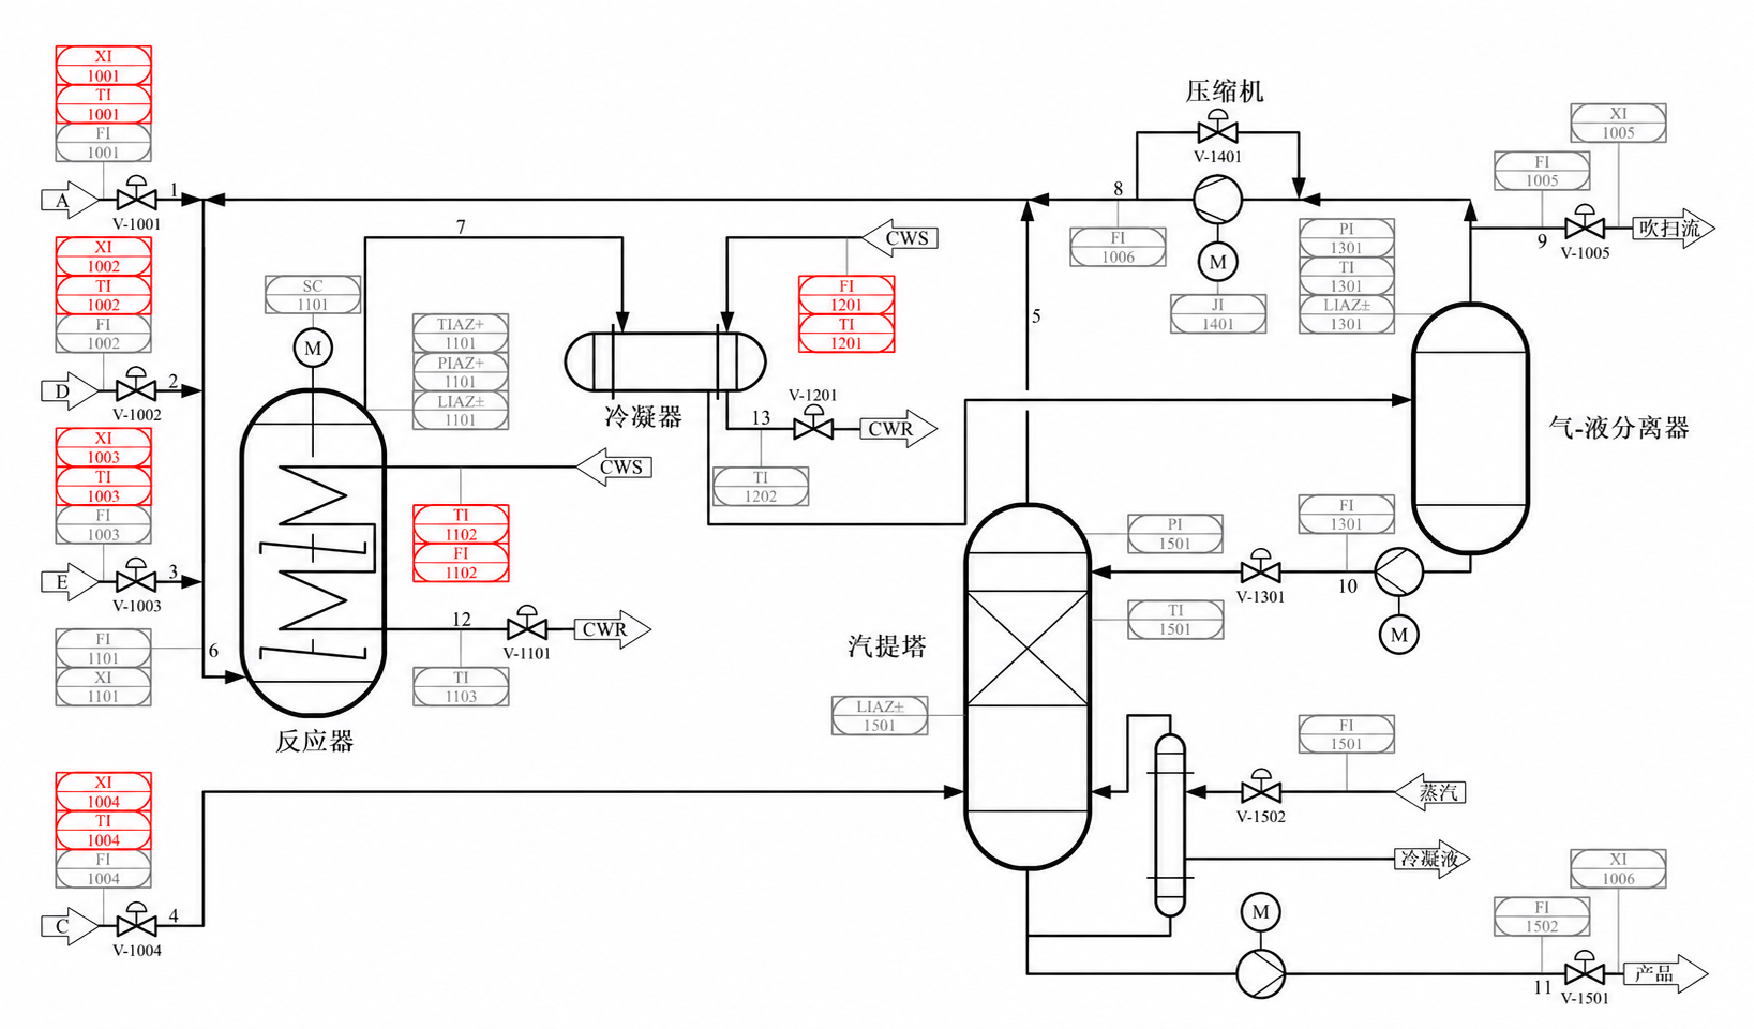
\includegraphics[width=1\textwidth]{figs/TEP.pdf}
    \caption{田纳西伊斯曼过程流程示意图}
    \label{fig:tep_process}
\end{figure}

从领域自适应角度看，TEP 数据集的主要特点是包含多个生产模式。不同生产模式对应不同的产品质量比和生产率，会改变过程变量之间的统计关系和数据概率分布。因此，在某一生产模式下训练得到的模型，直接迁移到另一生产模式时可能出现明显性能退化。配套基准研究通过变量相关矩阵和模式间 Wasserstein 距离分析表明，不同生产模式会造成可观的分布偏移\cite{montesuma2024benchmark}。因此，该数据集适合用于构造单源和多源跨工况领域自适应故障诊断任务。

数据集共包含 6 个生产模式，每个生产模式可视为一个领域。本文沿用基准文献的编号方式，将第 $r$ 个生产模式在公式和实验场景表中简记为 $m_r$，其中 $r=1,2,\cdots,6$。各生产模式的产品质量比、生产率和样本数如表 \ref{tab:tep_modes} 所示。

\begin{table}[!htbp]
    \centering
    \caption{田纳西伊斯曼过程领域自适应数据集中各生产模式信息}
    \label{tab:tep_modes}
    \zihao{5}
    \begin{tabular}{c c c c}
        \toprule
        生产模式 & G/H质量比 & 生产率 & 样本数 \\
        \midrule
        模式1 & 50/50 & 7038 kg/h G 和 7038 kg/h H & 2900 \\
        模式2 & 10/90 & 1408 kg/h G 和 12669 kg/h H & 2845 \\
        模式3 & 90/10 & 10000 kg/h G 和 1111 kg/h H & 2899 \\
        模式4 & 50/50 & 最大生产率 & 2865 \\
        模式5 & 10/90 & 最大生产率 & 2883 \\
        模式6 & 90/10 & 最大生产率 & 2897 \\
        \addlinespace
        合计 & -- & -- & 17289 \\
        \bottomrule
    \end{tabular}
\end{table}

在上述编号体系下，配套基准研究进一步指出，模式2与其他模式的分布差异相对较大，而模式3与模式6、模式1与模式4、模式5之间具有相对更接近的统计特性\cite{montesuma2024benchmark}。

数据集按照生产模式组织为多个领域，每个样本由多变量过程时间序列及其故障类别组成。对于第 $m$ 个生产模式，其样本集合可表示为
\begin{equation}
    \mathbf{X}^{(m)} \in \mathbb{R}^{N_m \times 600 \times 34},
\end{equation}
其中 $N_m$ 表示该模式下的样本数量，600 表示每个样本包含的时间步数，34 表示连续过程变量数量。标签空间为
\begin{equation}
    \mathcal{Y}=\{0,1,2,\cdots,28\},
\end{equation}
其中标签 0 表示正常状态，标签 1 至 28 分别表示 28 种故障类型。本文将每个样本视为一个多变量时间序列故障诊断样本，不同生产模式之间的同类故障样本构成跨工况迁移学习中的源域和目标域样本。

原始 TEP 仿真环境包含 53 个变量，其中部分变量为非连续变量。相关基准研究按照数据预处理规则选取 34 个连续变量作为诊断特征，包括测量变量 XME(1) 至 XME(22) 以及操纵变量 XMV(1) 至 XMV(12)\cite{montesuma2024benchmark}。由于不同过程变量的量纲和数值范围差异较大，本文对每个生产模式内部的每个变量进行标准化处理。对于生产模式 $m$ 中第 $j$ 个变量，其标准化过程为
\begin{equation}
    \tilde{x}_{i,t,j}^{(m)}
    =
    \frac{x_{i,t,j}^{(m)}-\bar{x}_{j}^{(m)}}{\sigma_{j}^{(m)}+\epsilon},
\end{equation}
其中 $x_{i,t,j}^{(m)}$ 表示第 $m$ 个生产模式中第 $i$ 个样本在时间步 $t$、变量 $j$ 上的原始取值，$\bar{x}_{j}^{(m)}$ 和 $\sigma_{j}^{(m)}$ 分别表示该生产模式下第 $j$ 个变量在所有样本和时间步上的均值与标准差，$\epsilon$ 为防止标准差为零导致数值不稳定的极小常数。该标准化过程仅使用样本统计量，不使用目标域标签信息。

\medskip
\noindent\textbf{数据划分与训练协议}

数据集提供五折样本划分。为控制实验规模并保证不同方法、不同迁移任务之间的可比性，本文采用固定第一折评估方式：目标域中属于第一折的样本作为测试集，仅在最终评价阶段使用其标签；目标域中不属于第一折的样本作为无标签目标训练数据参与领域自适应训练。源域样本则使用相同划分编号对应的训练部分及其标签参与源域监督训练。对于多源场景，所有源域均按照第一折对应训练部分构造有标签源域训练集，目标域仍只以无标签形式参与训练。正文结果均在统一数据划分和统一随机性控制下获得，以保证不同方法之间的比较口径一致。

以单源任务 $m_s \rightarrow m_t$ 为例，训练过程中可访问的数据包括源域有标签样本
\begin{equation}
    \mathcal{D}_{s}^{\mathrm{train}}
    =
    \{(x_i^{s},y_i^{s})\},
\end{equation}
以及目标域无标签样本
\begin{equation}
    \mathcal{D}_{t}^{\mathrm{train}}
    =
    \{x_j^{t}\}.
\end{equation}
目标域测试集记为
\begin{equation}
    \mathcal{D}_{t}^{\mathrm{test}}
    =
    \{(x_u^{t},y_u^{t})\},
\end{equation}
其中 $y_u^{t}$ 只用于最终计算评价指标，禁止在模型训练、伪标签筛选、超参数选择和早停过程中使用。多源任务 $m_{s_1}+m_{s_2}+\cdots+m_{s_K}\rightarrow m_t$ 的设置与单源任务类似，只是源域由一个扩展为多个。

目标域监督参考方法使用目标域训练部分的标签进行监督训练，不属于无监督领域自适应方法，也不参与无监督领域自适应方法的公平比较。由于其训练数据量、模型结构和训练设置可能与多源方法存在差异，本文不将其视为所有场景下的严格上界，而仅作为目标域有标签条件下的参考结果。

本文主要采用诊断准确率、宏平均 F1 值和平衡准确率作为评价指标。诊断准确率用于衡量整体分类正确比例；宏平均 F1 值对每个类别的 F1 值进行等权平均，更能反映多类别故障诊断中的少数类性能；平衡准确率对各类别召回率进行平均，可降低类别样本数量差异对评价结果的影响。对于目标域故障诊断任务，本文同时结合混淆矩阵和跨域特征可视化结果分析模型的类别混淆情况和特征对齐效果。

\medskip
\noindent\textbf{单源跨工况实验场景}

单源跨工况实验用于验证第三章和第四章提出的单源领域自适应方法。本文选取模式1、模式2和模式5构成单源实验子集，并按照双向迁移原则构造任务，即任意两个生产模式之间均进行双向迁移，每个模式既作为源域，也作为目标域。选择模式1、模式2和模式5的原因是：模式1与模式5在基准研究中属于相对接近的模式组，可用于分析分布偏移较弱任务中的方法增益；模式2与其他模式差异较大，可用于检验方法在困难跨工况任务中的适应能力\cite{montesuma2024benchmark}。

单源实验共包含 6 个任务，如表 \ref{tab:single_source_tasks} 所示，其中 $m_1$、$m_2$ 和 $m_5$ 的含义沿用上述生产模式记号。

\begin{table}[!htbp]
    \centering
    \caption{单源跨工况实验场景}
    \label{tab:single_source_tasks}
    \zihao{5}
    \begin{tabular}{c c c}
        \toprule
        序号 & 源域 & 目标域 \\
        \midrule
        1 & $m_1$ & $m_2$ \\
        2 & $m_2$ & $m_1$ \\
        3 & $m_1$ & $m_5$ \\
        4 & $m_5$ & $m_1$ \\
        5 & $m_2$ & $m_5$ \\
        6 & $m_5$ & $m_2$ \\
        \bottomrule
    \end{tabular}
\end{table}

在每个单源任务中，源域样本带有故障类别标签，目标域训练样本不提供标签。实验先用源域直接迁移方法评估直接跨工况泛化能力，再与典型领域自适应基线以及第三章、第四章方法进行比较，以验证时序原型非平衡联合分布对齐和多证据置信均衡伪标签学习对目标域诊断性能的影响。

\medskip
\noindent\textbf{多源跨工况实验场景}

多源跨工况实验用于验证第五章提出的类条件源域可靠性加权方法。与单源场景不同，多源领域自适应可以利用多个源域的有标签数据适配同一个目标域。多源设置能够提供更丰富的故障样本和生产模式信息，但也可能引入源域间分布差异和负迁移问题。因此，多源实验不仅关注模型是否能够利用更多源域数据，还关注模型是否能够识别不同源域对不同故障类别的可靠性差异。

本文多源实验包含两类任务。第一类为模式1、模式2和模式5之间的两源域跨工况任务，用于考察小规模多源条件下的迁移效果。该设置与单源双向迁移场景保持一致，只是每次选择两个模式作为源域，剩余一个模式作为目标域。具体任务如表 \ref{tab:two_source_tasks} 所示。

\begin{table}[!htbp]
    \centering
    \caption{生产模式1、生产模式2和生产模式5之间的两源域跨工况实验场景}
    \label{tab:two_source_tasks}
    \zihao{5}
    \begin{tabular}{c c c}
        \toprule
        序号 & 源域 & 目标域 \\
        \midrule
        1 & $m_1 + m_2$ & $m_5$ \\
        2 & $m_2 + m_5$ & $m_1$ \\
        3 & $m_1 + m_5$ & $m_2$ \\
        \bottomrule
    \end{tabular}
\end{table}

第二类为 6 个生产模式之间的五源域跨工况任务。该设置每次选择其中 1 个生产模式作为目标域，其余 5 个生产模式作为源域。该实验能够更全面地评估多源领域自适应方法在不同目标生产模式上的适用性，也更适合分析类条件源域可靠性矩阵是否能够刻画不同源域对不同故障类别的贡献。具体任务如表 \ref{tab:five_source_tasks} 所示。

\begin{table}[!htbp]
    \centering
    \caption{6个生产模式之间的五源域跨工况实验场景}
    \label{tab:five_source_tasks}
    \zihao{5}
    \begin{tabular}{c c c}
        \toprule
        序号 & 源域 & 目标域 \\
        \midrule
        1 & $m_2 + m_3 + m_4 + m_5 + m_6$ & $m_1$ \\
        2 & $m_1 + m_3 + m_4 + m_5 + m_6$ & $m_2$ \\
        3 & $m_1 + m_2 + m_4 + m_5 + m_6$ & $m_3$ \\
        4 & $m_1 + m_2 + m_3 + m_5 + m_6$ & $m_4$ \\
        5 & $m_1 + m_2 + m_3 + m_4 + m_6$ & $m_5$ \\
        6 & $m_1 + m_2 + m_3 + m_4 + m_5$ & $m_6$ \\
        \bottomrule
    \end{tabular}
\end{table}

在多源实验中，源域直接迁移方法用于衡量不进行领域自适应时的多源泛化能力，CoDATS 用于衡量卷积式时间序列领域自适应基线性能，WJDOT 用于衡量基于多源加权联合分布最优传输的基线性能，本文第五章方法用于验证类条件源域可靠性加权机制的有效性。通过两源域和五源域两组实验，可以分别分析源域数量较少和源域数量较多时，源域可靠性建模对目标域故障诊断结果的影响。

\section{方法有效性验证}

本节按照第三章、第四章和第五章方法的递进关系组织代表场景分析。第 6.3.1 节验证 SourceOnly $\rightarrow$ DeepJDOT $\rightarrow$ TPU-DeepJDOT 的递进关系；第 6.3.2 节验证 TPU-DeepJDOT $\rightarrow$ CBTPU-DeepJDOT 的伪标签细化效果；第 6.3.3 节验证 SourceOnly $\rightarrow$ CA-CCSR-WJDOT 的多源选择性迁移效果。为避免将全局热力图和局部图像证据混在一起，本节只使用混淆矩阵、域 t-SNE 和类 t-SNE 三类图像进行对比；跨迁移任务的整体性能与基线优势留到第 6.4 节集中讨论。

单源代表场景按验证目标分别选取：第 6.3.1 节采用 $m_5\rightarrow m_2$ 任务，用于观察第三章方法相对 SourceOnly 和 DeepJDOT 的主线增益；第 6.3.2 节采用 $m_5\rightarrow m_1$ 任务，用于观察第四章伪标签细化阶段的补充收益。多源代表场景选取五源域跨工况任务 $\{m_1,m_3,m_4,m_5,m_6\}\rightarrow m_2$，用于观察引入多个源域后类条件源域可靠性建模的作用。

\subsection{时序原型非平衡联合分布对齐有效性验证}

本小节验证第三章方法的核心问题：在单源跨工况诊断中，SourceOnly 缺少领域对齐，DeepJDOT 引入联合分布最优传输，TPU-DeepJDOT 进一步加入非平衡传输、源域类别原型和时序统计代价。若第三章方法有效，则代表场景中应当出现 SourceOnly $<$ DeepJDOT $<$ TPU-DeepJDOT 的递进趋势，即目标域混淆减少、源目标域分布更加接近、类别结构更加清晰。

图 \ref{fig:ch6_tpu_mainline_confusion} 给出 $m_5\rightarrow m_2$ 任务中三种方法的目标域混淆矩阵。SourceOnly 的非对角元素较分散，说明仅依赖源域监督训练难以直接适应目标生产模式；DeepJDOT 能够缓解部分误判，但仍存在若干类别被吸收到错误预测类别的现象；TPU-DeepJDOT 的对角线响应更集中，说明时序原型非平衡联合分布对齐能够降低不可靠强制匹配对类别边界的干扰。该代表场景中，三者准确率分别为 56.08\%、67.20\% 和 83.60\%，形成明显递进关系。

\begin{figure}[!htbp]
    \centering
    \begin{subfigure}[b]{0.32\textwidth}
        \centering
        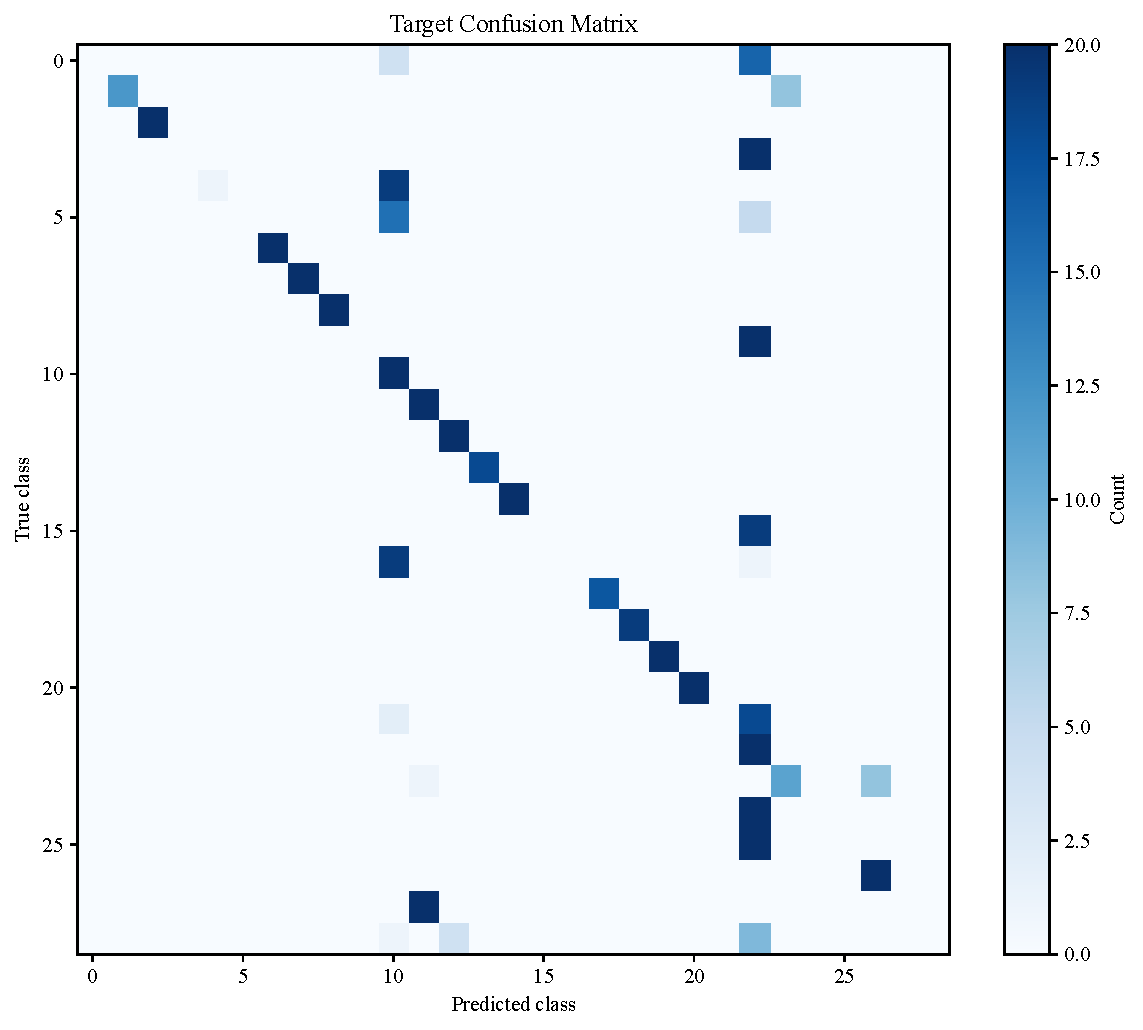
\includegraphics[width=\linewidth]{figs/ch6_single_sourceonly_5_to_2_confusion.pdf}
        \caption{SourceOnly}
    \end{subfigure}
    \hfill
    \begin{subfigure}[b]{0.32\textwidth}
        \centering
        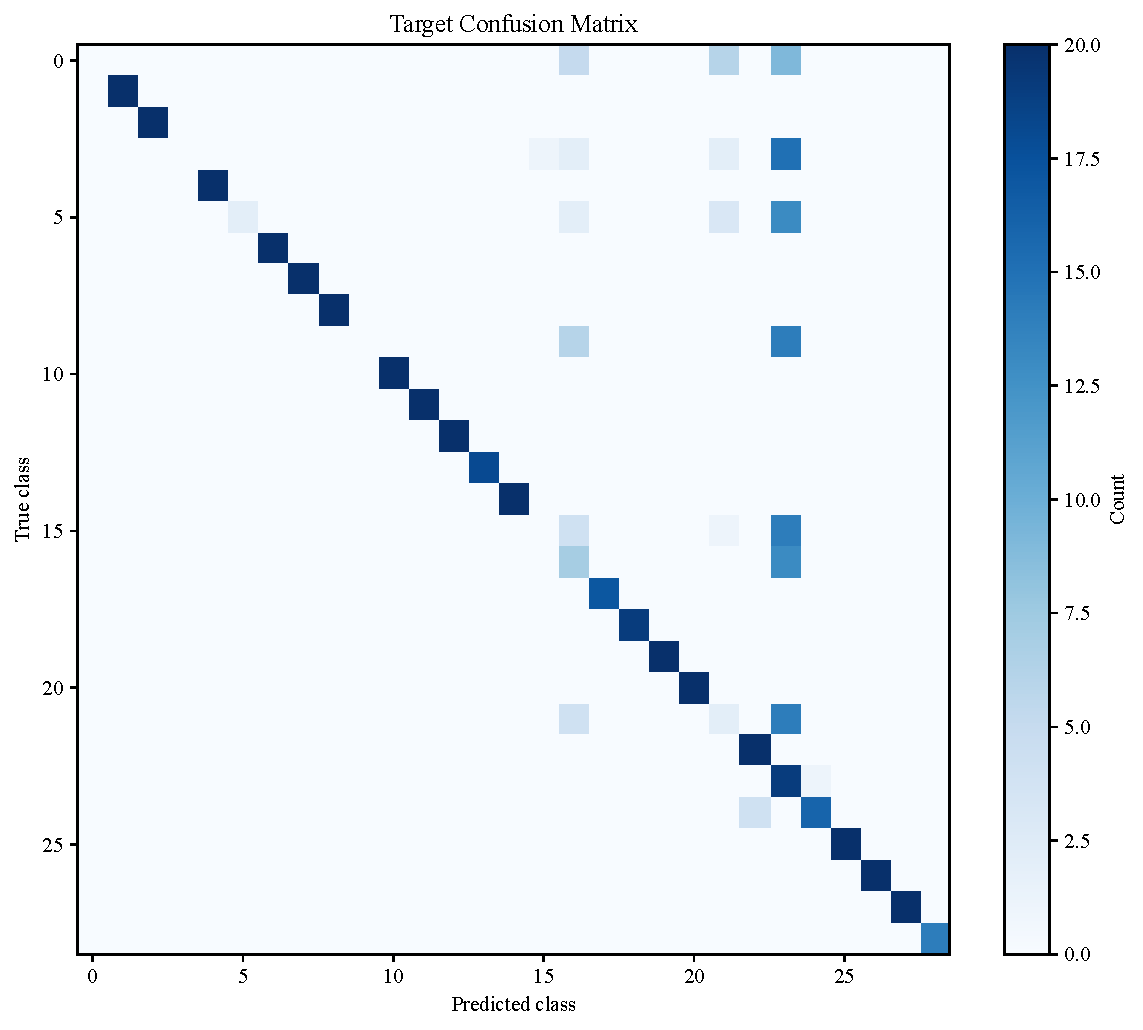
\includegraphics[width=\linewidth]{figs/ch6_single_deepjdot_5_to_2_confusion.pdf}
        \caption{DeepJDOT}
    \end{subfigure}
    \hfill
    \begin{subfigure}[b]{0.32\textwidth}
        \centering
        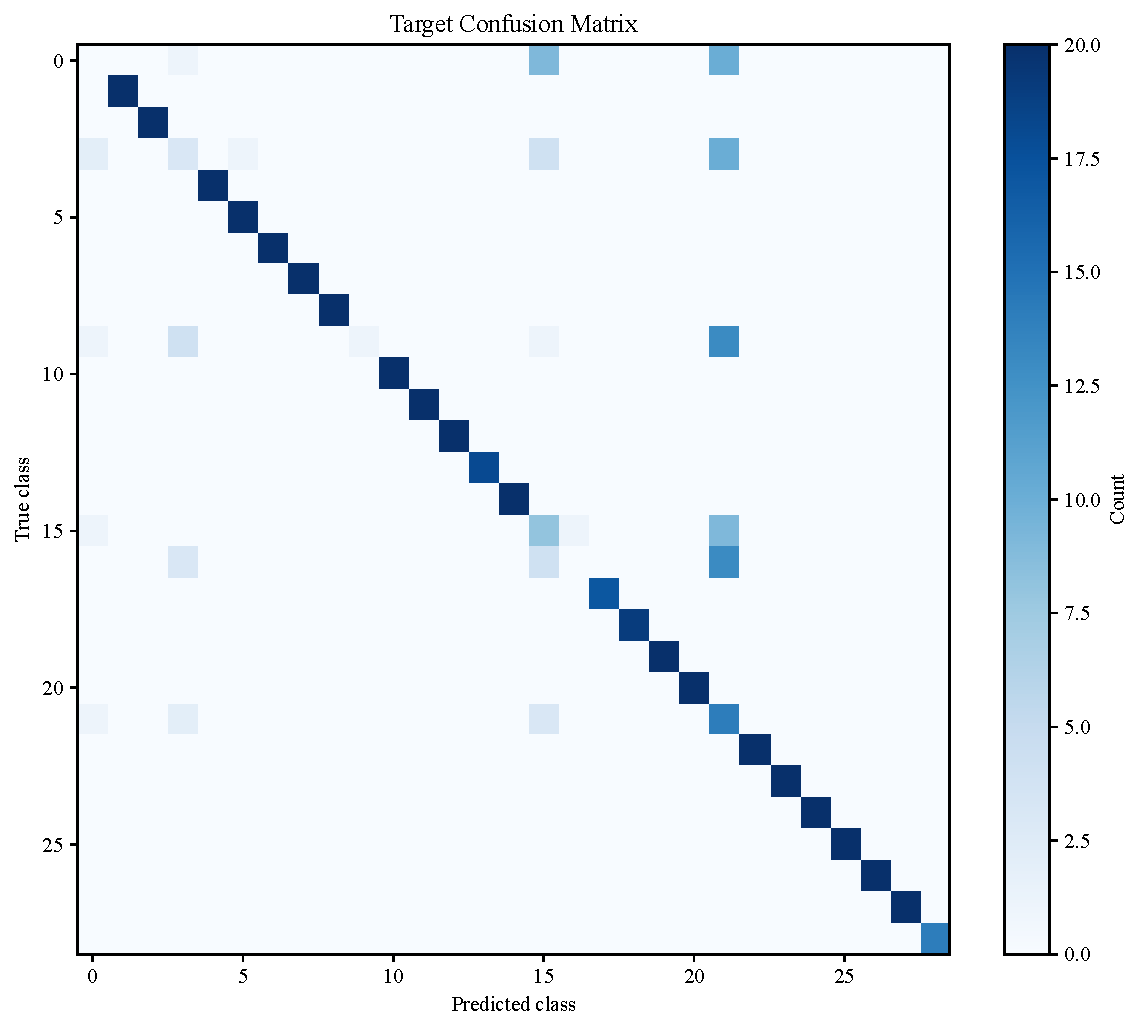
\includegraphics[width=\linewidth]{figs/ch6_single_TPU_DPJDOT_5_to_2_confusion.pdf}
        \caption{TPU-DeepJDOT}
    \end{subfigure}
    \caption{单源任务 $m_5\rightarrow m_2$ 中 SourceOnly、DeepJDOT 和 TPU-DeepJDOT 的目标域混淆矩阵对比}
    \label{fig:ch6_tpu_mainline_confusion}
\end{figure}

图 \ref{fig:ch6_tpu_mainline_tsne_domain} 从域分布角度展示同一任务的 t-SNE 结果。SourceOnly 下源域与目标域特征仍存在明显分离；DeepJDOT 缩短了部分源目标特征距离，但目标域样本仍有较多游离区域；TPU-DeepJDOT 使更多目标样本进入源域类别结构附近。该现象说明 TPU-DeepJDOT 的提升不是单纯依赖分类器输出校正，而是在特征层面改善了跨域对齐状态。

\begin{figure}[!htbp]
    \centering
    \begin{subfigure}[b]{0.32\textwidth}
        \centering
        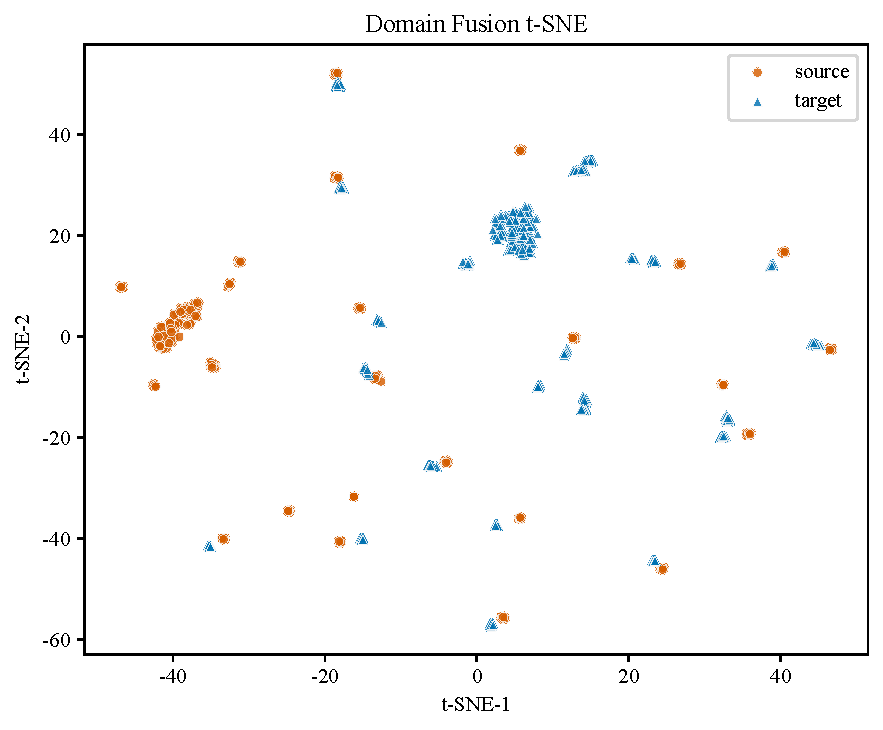
\includegraphics[width=\linewidth]{figs/ch6_single_sourceonly_5_to_2_tsne_domain.pdf}
        \caption{SourceOnly}
    \end{subfigure}
    \hfill
    \begin{subfigure}[b]{0.32\textwidth}
        \centering
        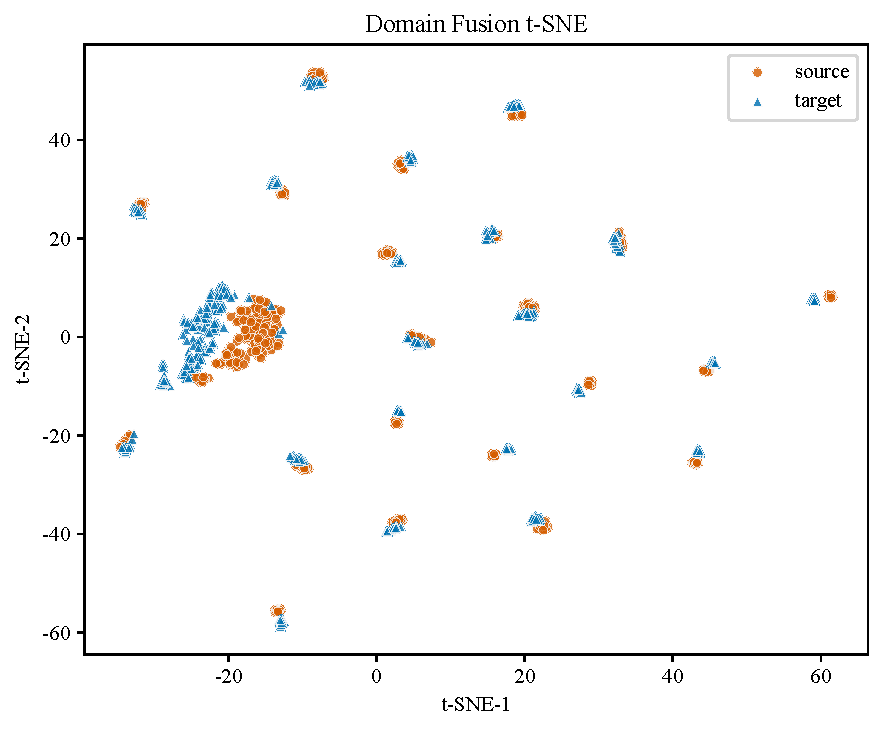
\includegraphics[width=\linewidth]{figs/ch6_single_deepjdot_5_to_2_tsne_domain.pdf}
        \caption{DeepJDOT}
    \end{subfigure}
    \hfill
    \begin{subfigure}[b]{0.32\textwidth}
        \centering
        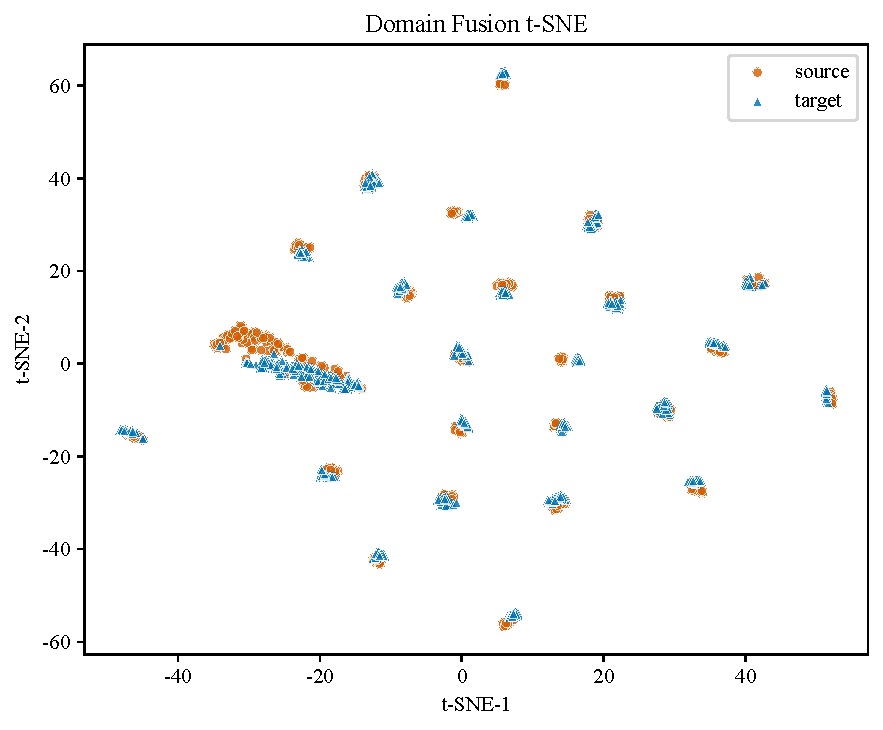
\includegraphics[width=\linewidth]{figs/ch6_single_TPU_DPJDOT_5_to_2_tsne_domain.pdf}
        \caption{TPU-DeepJDOT}
    \end{subfigure}
    \caption{单源任务 $m_5\rightarrow m_2$ 中 SourceOnly、DeepJDOT 和 TPU-DeepJDOT 的域 t-SNE 对比}
    \label{fig:ch6_tpu_mainline_tsne_domain}
\end{figure}

图 \ref{fig:ch6_tpu_mainline_tsne_class} 进一步从类别聚集角度比较三种方法。SourceOnly 的部分类别簇边界混杂，目标样本难以稳定落入正确类别区域；DeepJDOT 形成了一定类别聚集结构，但局部类别仍交叠；TPU-DeepJDOT 的类别簇更紧凑，且不同故障类别之间的分离度更好。这与第三章方法引入源域类别原型、时序统计代价和源域监督对比学习的设计目标一致。

\begin{figure}[!htbp]
    \centering
    \begin{subfigure}[b]{0.32\textwidth}
        \centering
        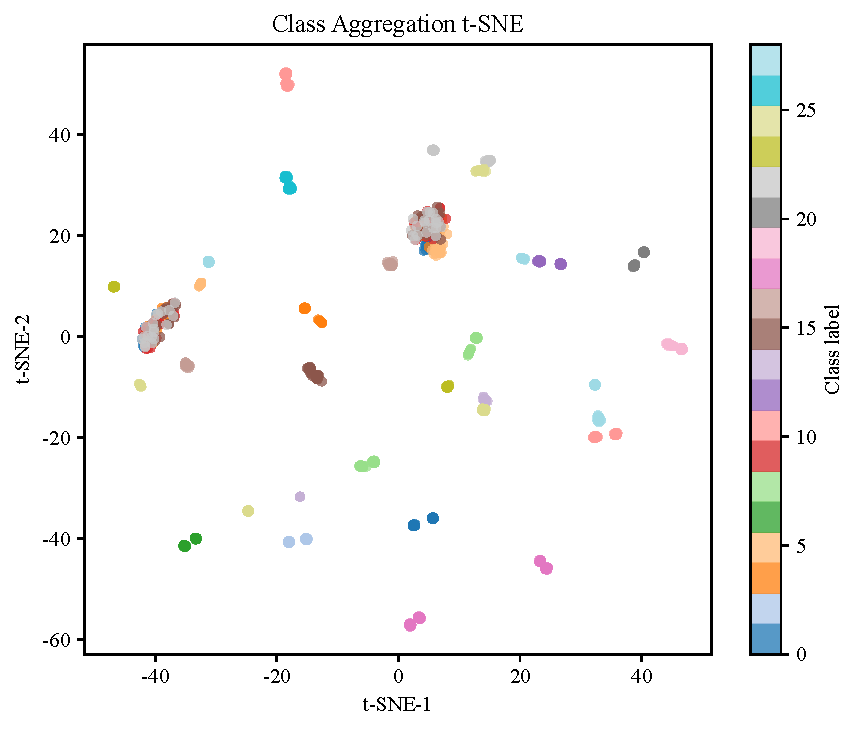
\includegraphics[width=\linewidth]{figs/ch6_single_sourceonly_5_to_2_tsne_class.pdf}
        \caption{SourceOnly}
    \end{subfigure}
    \hfill
    \begin{subfigure}[b]{0.32\textwidth}
        \centering
        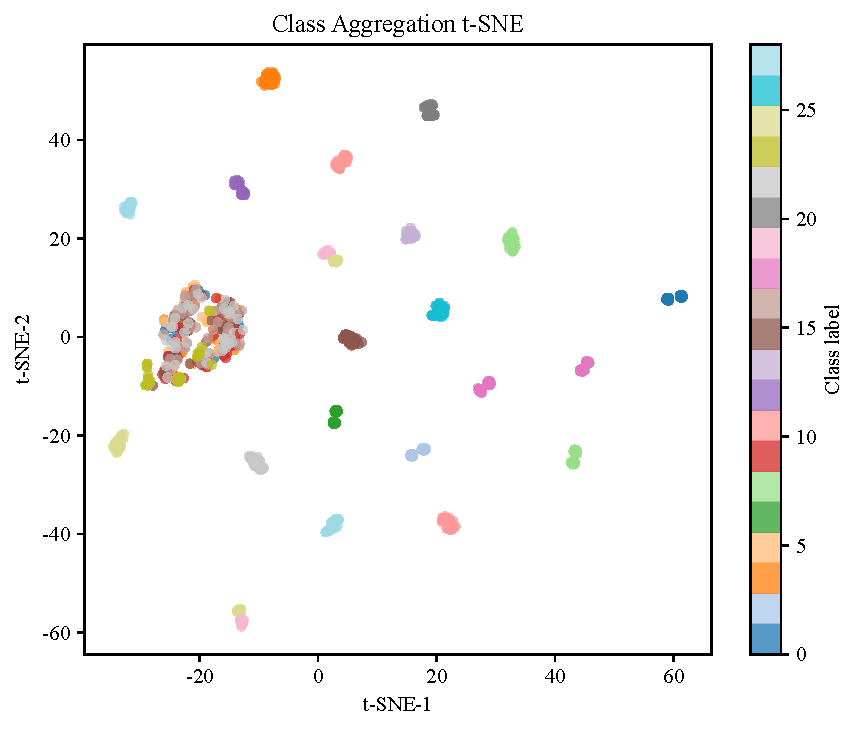
\includegraphics[width=\linewidth]{figs/ch6_single_deepjdot_5_to_2_tsne_class.pdf}
        \caption{DeepJDOT}
    \end{subfigure}
    \hfill
    \begin{subfigure}[b]{0.32\textwidth}
        \centering
        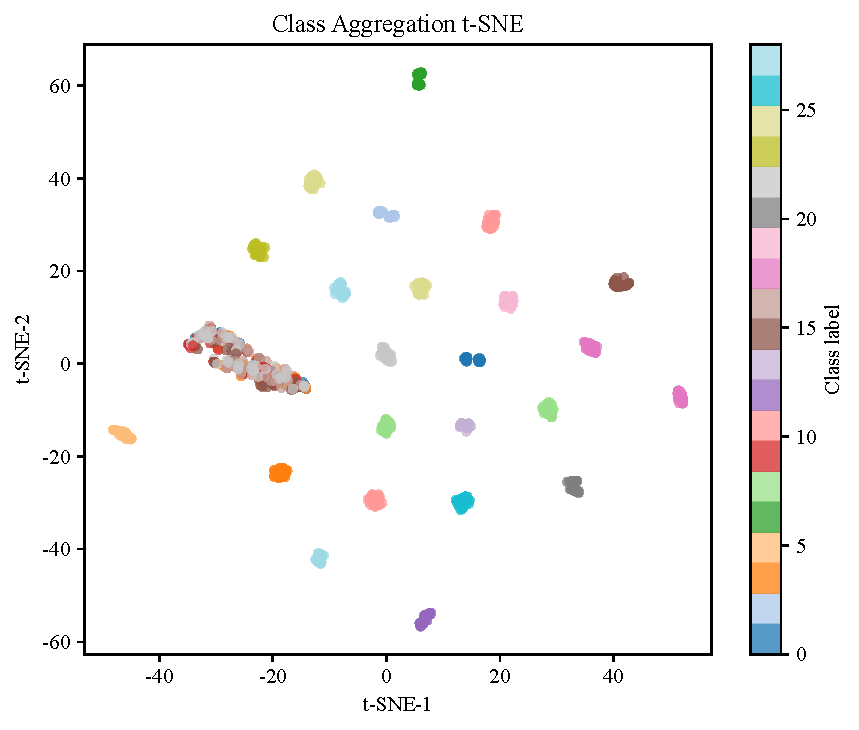
\includegraphics[width=\linewidth]{figs/ch6_single_TPU_DPJDOT_5_to_2_tsne_class.pdf}
        \caption{TPU-DeepJDOT}
    \end{subfigure}
    \caption{单源任务 $m_5\rightarrow m_2$ 中 SourceOnly、DeepJDOT 和 TPU-DeepJDOT 的类 t-SNE 对比}
    \label{fig:ch6_tpu_mainline_tsne_class}
\end{figure}

综合混淆矩阵、域 t-SNE 和类 t-SNE 可以看出，TPU-DeepJDOT 相比 DeepJDOT 的主要收益来自更可靠的类别结构保持。非平衡传输允许削减低可靠匹配质量，原型代价和时序统计代价则使传输计划不只依赖瞬时特征距离，从而在目标域无标签条件下减少错误对齐。

\subsection{多证据置信均衡伪标签有效性验证}

本小节验证第四章方法的核心问题：在 TPU-DeepJDOT 已经建立较可靠源目标对齐关系之后，CBTPU-DeepJDOT 是否能够通过多证据置信筛选和类别均衡伪标签学习进一步改善目标域决策边界。与第 6.3.1 节不同，本小节不再重复 SourceOnly 和 DeepJDOT 的完整递进链，而是直接比较 TPU-DeepJDOT 与 CBTPU-DeepJDOT。

图 \ref{fig:ch6_cbtpu_confusion} 展示两种方法在 $m_5\rightarrow m_1$ 任务上的混淆矩阵。CBTPU-DeepJDOT 相比 TPU-DeepJDOT 的代表场景准确率由 77.59\% 提升到 81.38\%，宏平均 F1 由 76.06\% 提升到 81.10\%，平衡准确率由 77.59\% 提升到 81.38\%。该提升幅度小于第 6.3.1 节中 DeepJDOT 到 TPU-DeepJDOT 的跃升，但混淆矩阵中局部非对角误判继续减弱，说明伪标签阶段主要承担细化目标域边界的作用。

\begin{figure}[!htbp]
    \centering
    \begin{subfigure}[b]{0.48\textwidth}
        \centering
        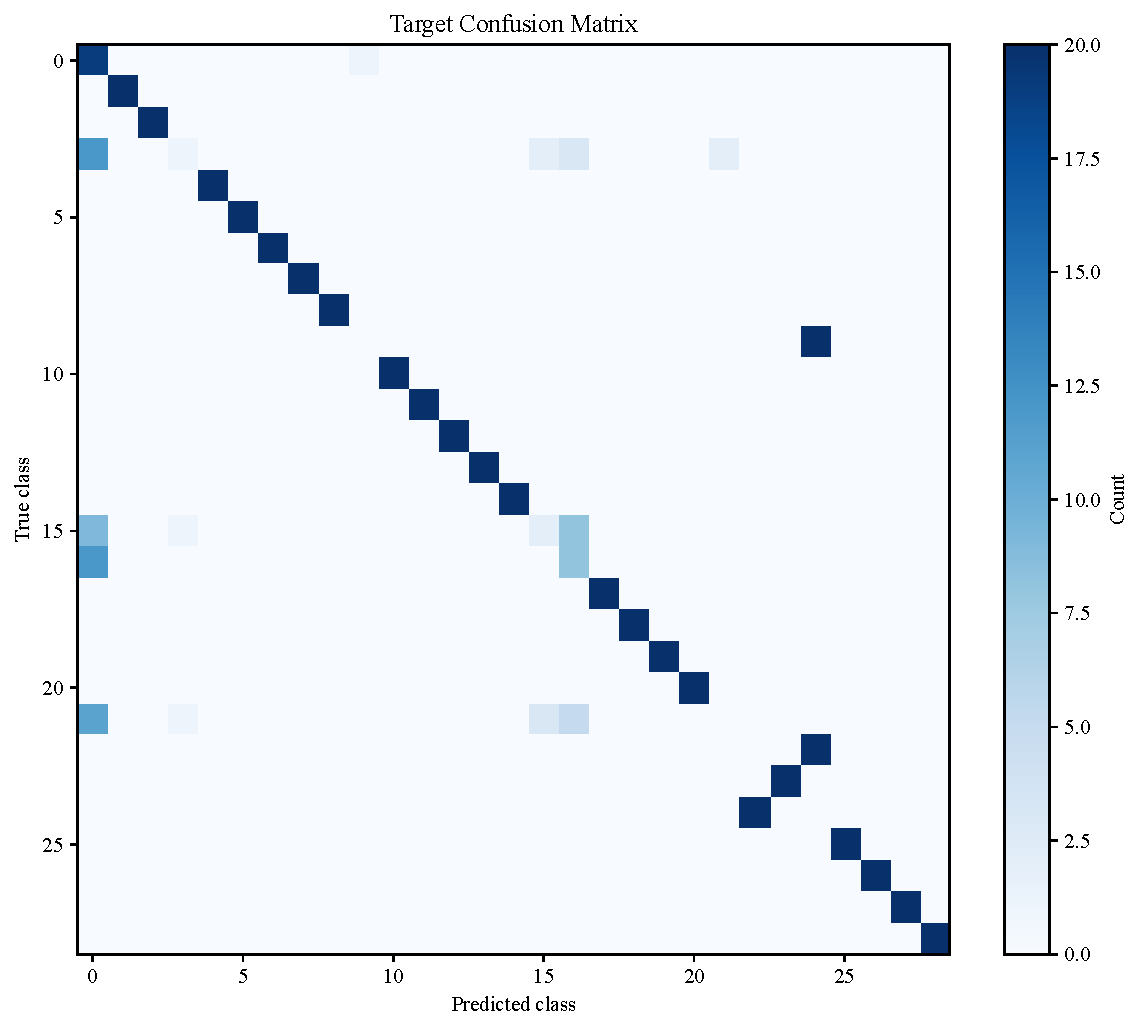
\includegraphics[width=\linewidth]{figs/ch6_single_TPU_DPJDOT_5_to_1_confusion.pdf}
        \caption{TPU-DeepJDOT}
    \end{subfigure}
    \hfill
    \begin{subfigure}[b]{0.48\textwidth}
        \centering
        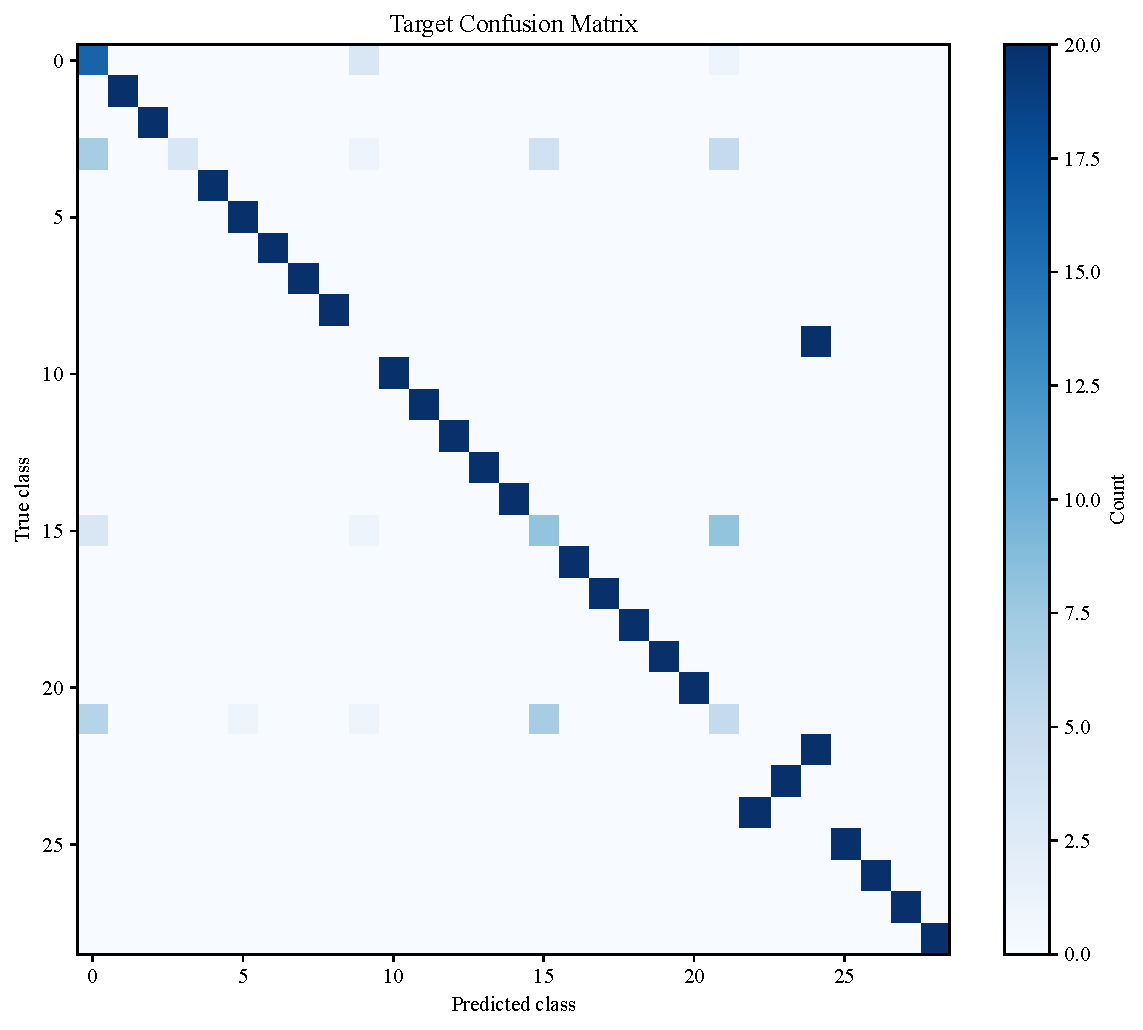
\includegraphics[width=\linewidth]{figs/ch6_single_CBTPU_DPJDOT_5_to_1_confusion.pdf}
        \caption{CBTPU-DeepJDOT}
    \end{subfigure}
    \caption{单源任务 $m_5\rightarrow m_1$ 中 TPU-DeepJDOT 和 CBTPU-DeepJDOT 的目标域混淆矩阵对比}
    \label{fig:ch6_cbtpu_confusion}
\end{figure}

图 \ref{fig:ch6_cbtpu_tsne_domain} 从域 t-SNE 角度比较 TPU-DeepJDOT 与 CBTPU-DeepJDOT。两者都已经形成较好的源目标融合结构，这说明第四章方法并不是重新建立跨域对齐，而是在第三章对齐基础上进行保守微调。CBTPU-DeepJDOT 中部分目标样本在主簇附近更加紧凑，反映出高置信目标样本被逐步纳入训练后，对目标域局部边界产生了细化作用。

\begin{figure}[!htbp]
    \centering
    \begin{subfigure}[b]{0.48\textwidth}
        \centering
        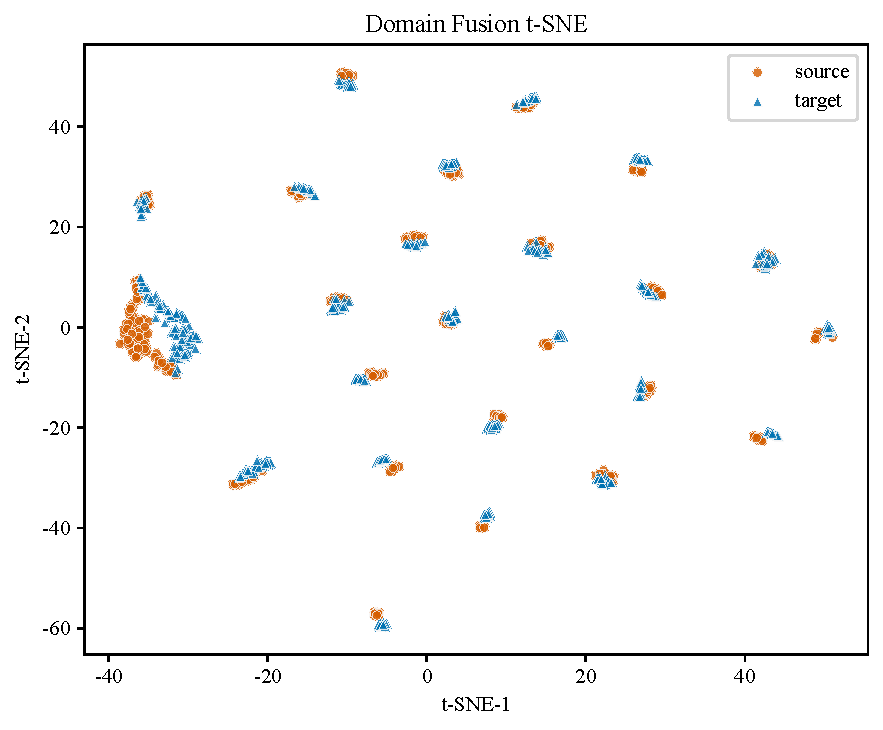
\includegraphics[width=\linewidth]{figs/ch6_single_TPU_DPJDOT_5_to_1_tsne_domain.pdf}
        \caption{TPU-DeepJDOT}
    \end{subfigure}
    \hfill
    \begin{subfigure}[b]{0.48\textwidth}
        \centering
        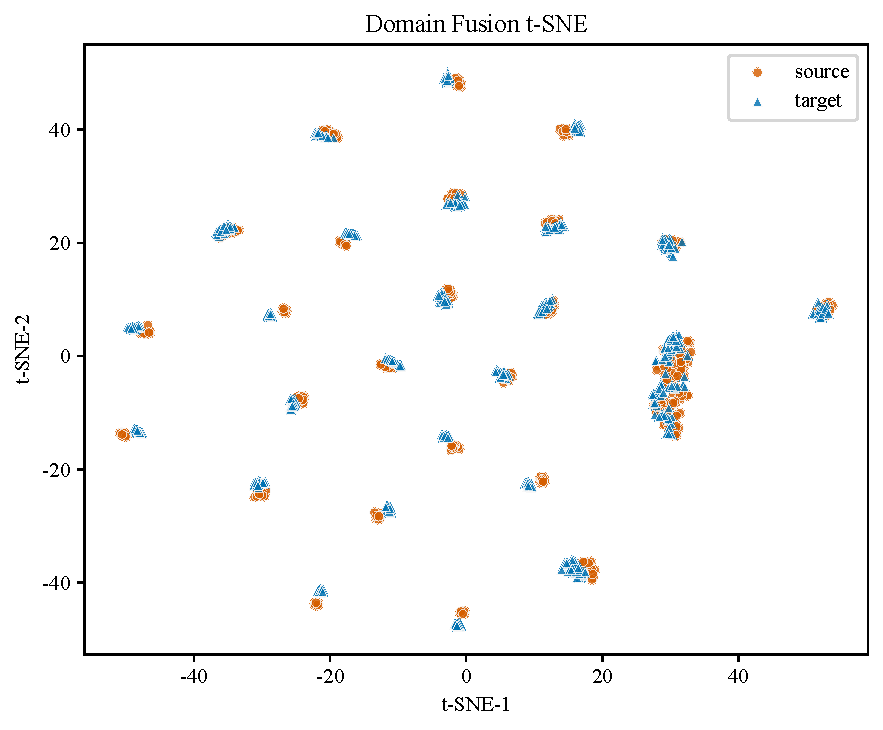
\includegraphics[width=\linewidth]{figs/ch6_single_CBTPU_DPJDOT_5_to_1_tsne_domain.pdf}
        \caption{CBTPU-DeepJDOT}
    \end{subfigure}
    \caption{单源任务 $m_5\rightarrow m_1$ 中 TPU-DeepJDOT 和 CBTPU-DeepJDOT 的域 t-SNE 对比}
    \label{fig:ch6_cbtpu_tsne_domain}
\end{figure}

图 \ref{fig:ch6_cbtpu_tsne_class} 给出类 t-SNE 对比。CBTPU-DeepJDOT 在保持 TPU-DeepJDOT 类别结构的同时，使部分目标样本进一步靠近对应类别簇。由于第四章方法只接受传输语义、教师预测语义和原型语义相对一致的目标样本，该变化体现出“保守使用目标域样本”的特点：其目标不是扩大伪标签覆盖率，而是降低错误伪标签进入训练目标的风险。

\begin{figure}[!htbp]
    \centering
    \begin{subfigure}[b]{0.48\textwidth}
        \centering
        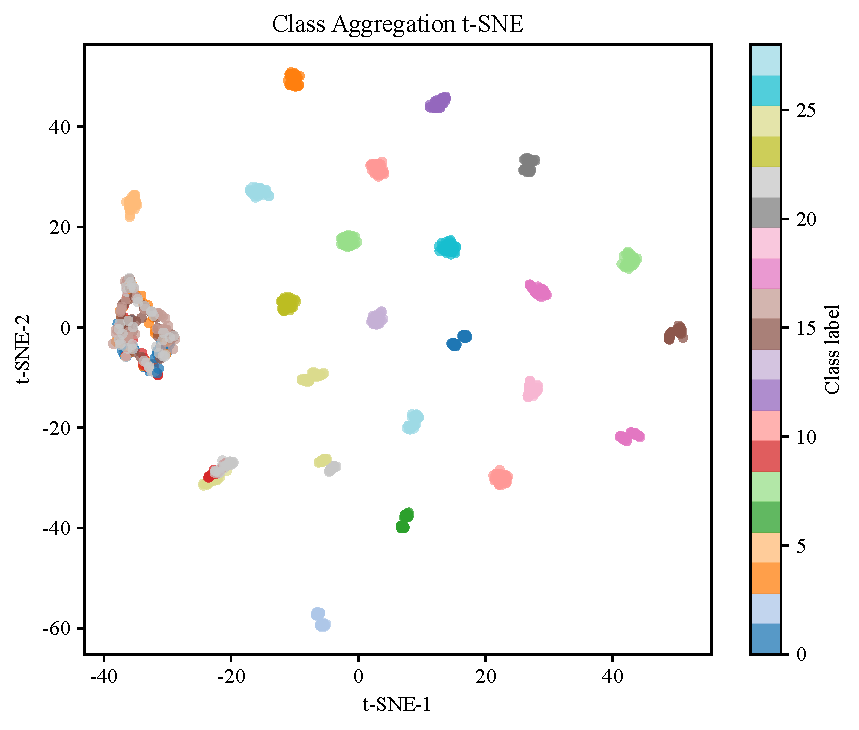
\includegraphics[width=\linewidth]{figs/ch6_single_TPU_DPJDOT_5_to_1_tsne_class.pdf}
        \caption{TPU-DeepJDOT}
    \end{subfigure}
    \hfill
    \begin{subfigure}[b]{0.48\textwidth}
        \centering
        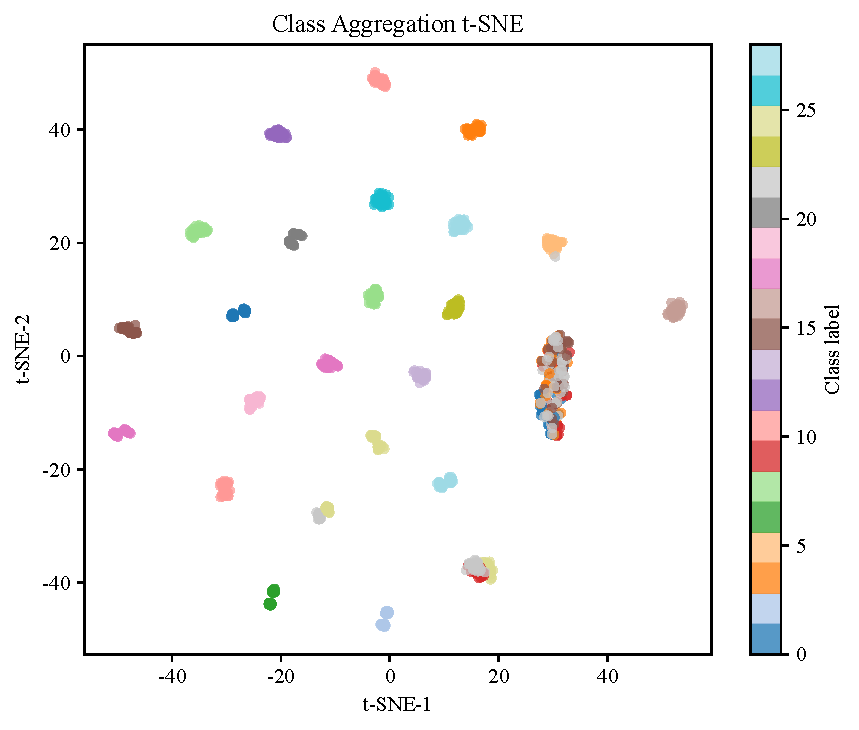
\includegraphics[width=\linewidth]{figs/ch6_single_CBTPU_DPJDOT_5_to_1_tsne_class.pdf}
        \caption{CBTPU-DeepJDOT}
    \end{subfigure}
    \caption{单源任务 $m_5\rightarrow m_1$ 中 TPU-DeepJDOT 和 CBTPU-DeepJDOT 的类 t-SNE 对比}
    \label{fig:ch6_cbtpu_tsne_class}
\end{figure}

因此，CBTPU-DeepJDOT 的有效性应理解为第二阶段增益：在 TPU-DeepJDOT 已经显著改善对齐结构后，进一步通过固定教师参考模型、传输计划、源域原型和类别均衡机制筛选可信目标样本，使目标域决策边界获得小幅但稳定的修正。

\subsection{类条件源域可靠性加权有效性验证}

本小节验证第五章方法的核心问题：多源设置中仅增加源域数量并不必然带来可靠迁移，模型还需要识别不同源域对不同故障类别的贡献差异。为突出 CA-CCSR-WJDOT 相对直接多源训练的作用，本小节比较五源 SourceOnly 与 CA-CCSR-WJDOT。完整的 CoDATS、WJDOT 等基线优势在第 6.4.2 节结合热力图、平均柱状图和平均性能表讨论。

图 \ref{fig:ch6_caccsr_confusion} 展示五源域跨工况任务 $\{m_1,m_3,m_4,m_5,m_6\}\rightarrow m_2$ 中 SourceOnly 与 CA-CCSR-WJDOT 的混淆矩阵。SourceOnly 虽然使用了多个源域的有标签样本，但目标域准确率只有 64.02\%，说明简单合并多源数据仍会受到跨工况偏移和源域差异影响。CA-CCSR-WJDOT 的目标域准确率达到 82.89\%，宏平均 F1 和平衡准确率分别达到 81.77\% 和 82.57\%，混淆矩阵中对角线响应明显增强，表明类条件源域可靠性加权能够显著减少目标域误判。

\begin{figure}[!htbp]
    \centering
    \begin{subfigure}[b]{0.48\textwidth}
        \centering
        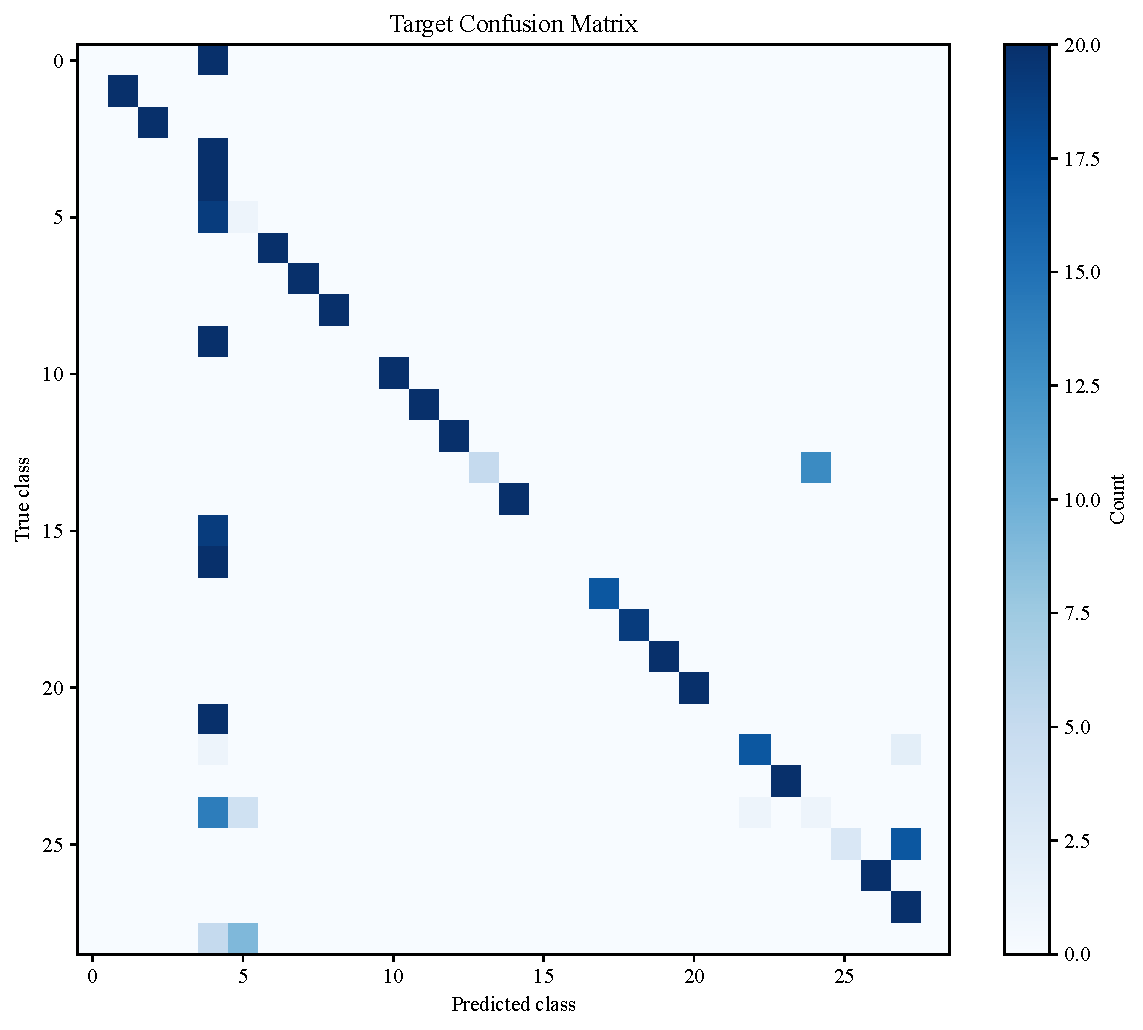
\includegraphics[width=\linewidth]{figs/ch6_multi_sourceonly_5src_to_2_confusion.pdf}
        \caption{SourceOnly}
    \end{subfigure}
    \hfill
    \begin{subfigure}[b]{0.48\textwidth}
        \centering
        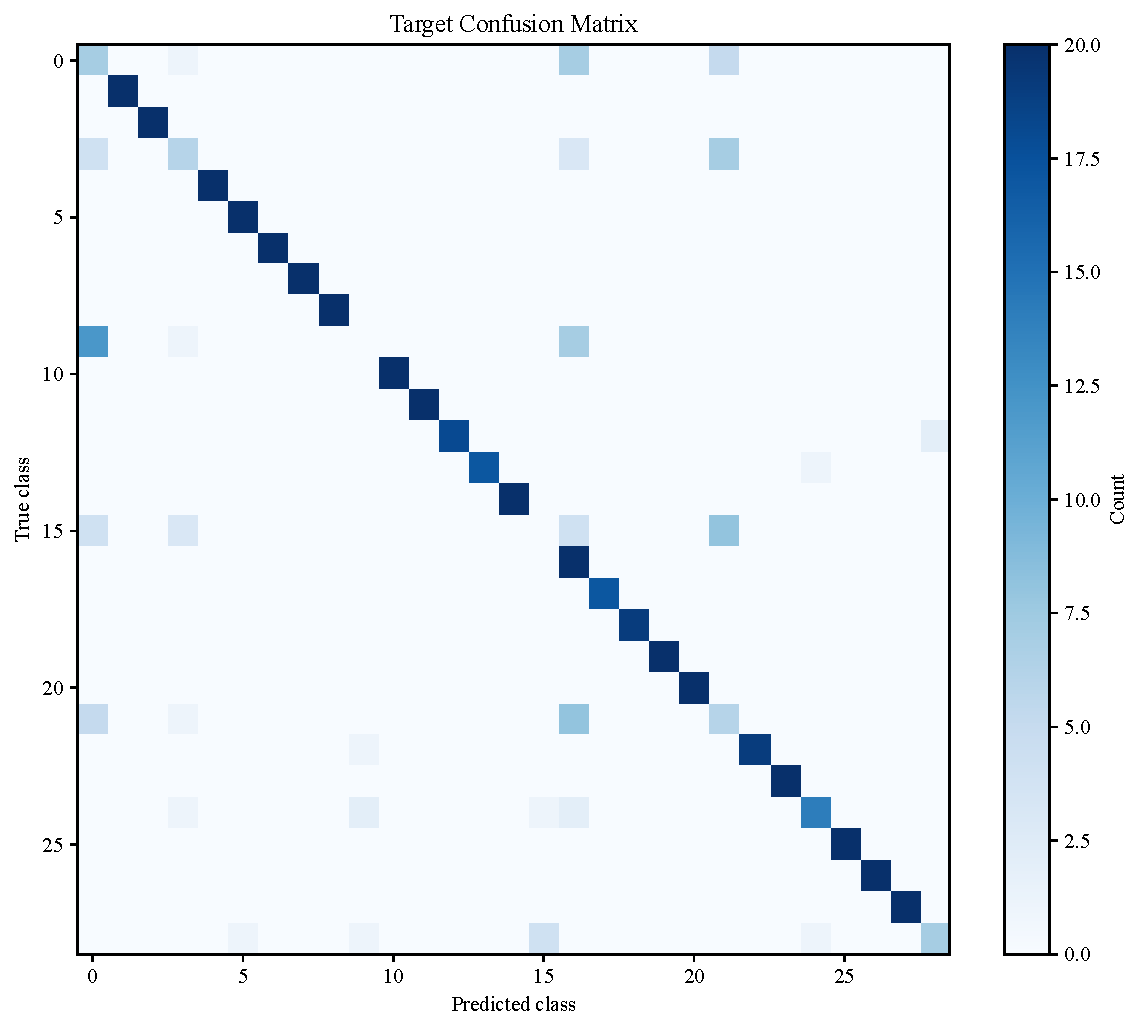
\includegraphics[width=\linewidth]{figs/ch6_multi_CA_CCSR_WJDOT_5src_to_2_confusion.pdf}
        \caption{CA-CCSR-WJDOT}
    \end{subfigure}
    \caption{五源域跨工况任务 $\{m_1,m_3,m_4,m_5,m_6\}\rightarrow m_2$ 中 SourceOnly 和 CA-CCSR-WJDOT 的目标域混淆矩阵对比}
    \label{fig:ch6_caccsr_confusion}
\end{figure}

图 \ref{fig:ch6_caccsr_tsne_domain} 展示两种方法的域 t-SNE 对比。SourceOnly 中目标域样本在多个区域与源域簇保持距离，说明多源监督训练本身不足以消除目标域偏移。CA-CCSR-WJDOT 中目标域样本更稳定地靠近多源特征结构，说明逐源联合分布对齐与类条件源域加权共同改善了目标域样本的位置。

\begin{figure}[!htbp]
    \centering
    \begin{subfigure}[b]{0.48\textwidth}
        \centering
        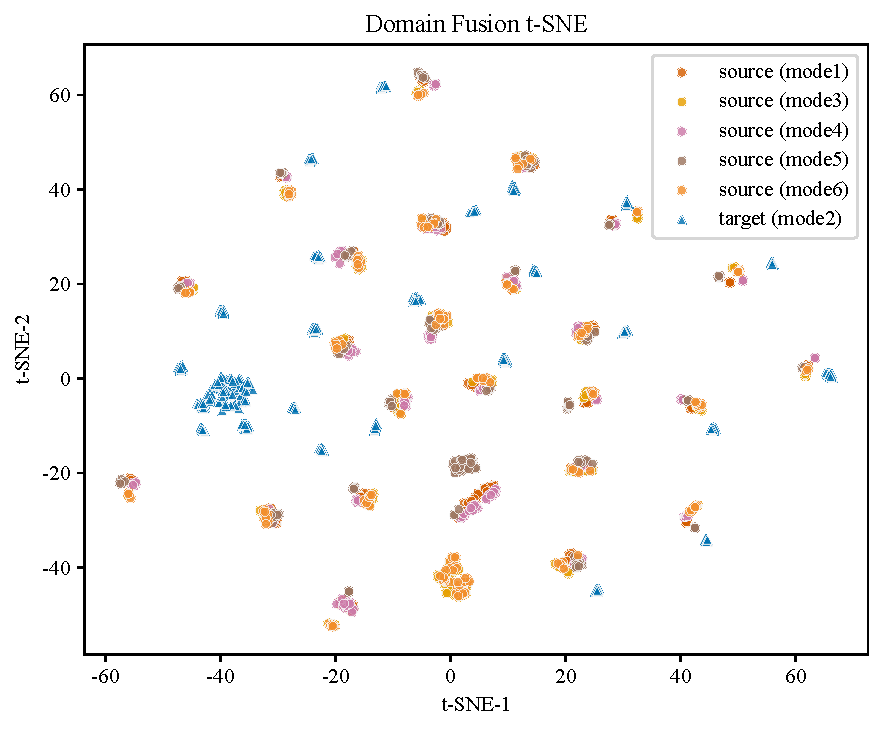
\includegraphics[width=\linewidth]{figs/ch6_multi_sourceonly_5src_to_2_tsne_domain.pdf}
        \caption{SourceOnly}
    \end{subfigure}
    \hfill
    \begin{subfigure}[b]{0.48\textwidth}
        \centering
        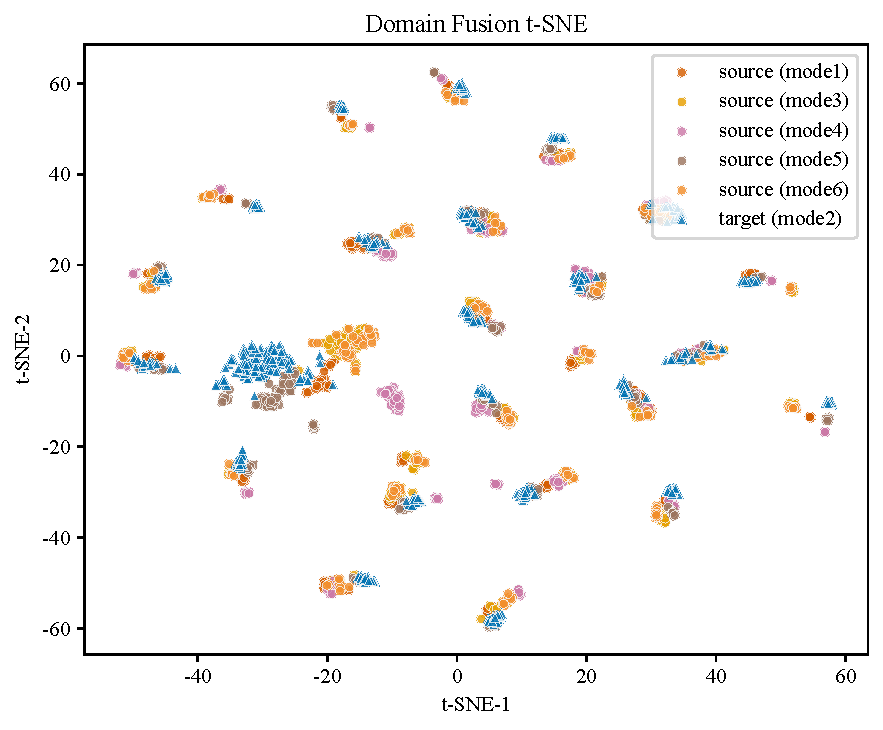
\includegraphics[width=\linewidth]{figs/ch6_multi_CA_CCSR_WJDOT_5src_to_2_tsne_domain.pdf}
        \caption{CA-CCSR-WJDOT}
    \end{subfigure}
    \caption{五源域跨工况任务 $\{m_1,m_3,m_4,m_5,m_6\}\rightarrow m_2$ 中 SourceOnly 和 CA-CCSR-WJDOT 的域 t-SNE 对比}
    \label{fig:ch6_caccsr_tsne_domain}
\end{figure}

图 \ref{fig:ch6_caccsr_tsne_class} 从类别结构角度进一步说明该差异。SourceOnly 的部分类别簇存在交叠，目标样本分布较分散；CA-CCSR-WJDOT 中类别簇结构更清晰，目标样本与对应类别区域的关系更稳定。这说明第五章方法的收益不仅来自更多源域样本，也来自对源域--故障类别可靠性的细粒度建模。

\begin{figure}[!htbp]
    \centering
    \begin{subfigure}[b]{0.48\textwidth}
        \centering
        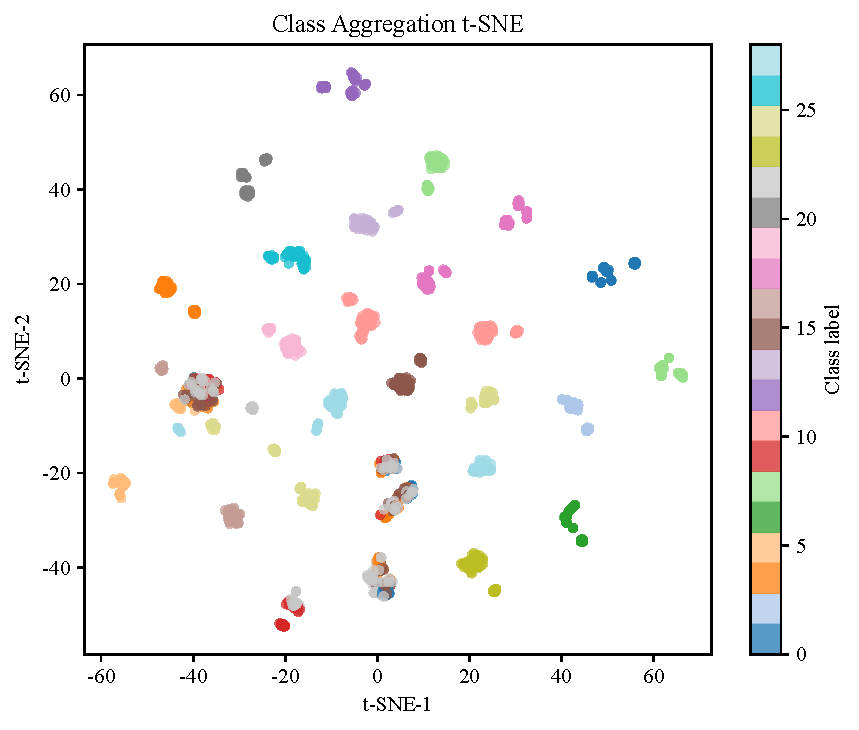
\includegraphics[width=\linewidth]{figs/ch6_multi_sourceonly_5src_to_2_tsne_class.pdf}
        \caption{SourceOnly}
    \end{subfigure}
    \hfill
    \begin{subfigure}[b]{0.48\textwidth}
        \centering
        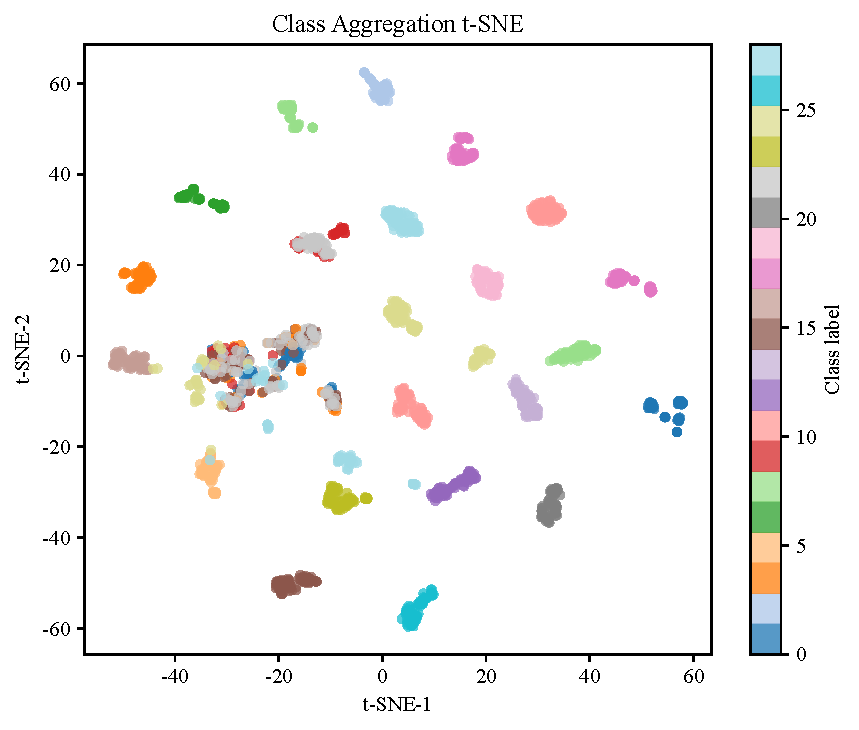
\includegraphics[width=\linewidth]{figs/ch6_multi_CA_CCSR_WJDOT_5src_to_2_tsne_class.pdf}
        \caption{CA-CCSR-WJDOT}
    \end{subfigure}
    \caption{五源域跨工况任务 $\{m_1,m_3,m_4,m_5,m_6\}\rightarrow m_2$ 中 SourceOnly 和 CA-CCSR-WJDOT 的类 t-SNE 对比}
    \label{fig:ch6_caccsr_tsne_class}
\end{figure}

由上述三类图像可以看出，CA-CCSR-WJDOT 相比多源 SourceOnly 同时改善了类别预测、域间融合和类别聚集结构。这一结果验证了第五章方法的基本假设：多源跨工况诊断不能只依赖源域数量增加，还需要在类别层面判断各源域是否可靠。

\section{综合实验结果对比分析}

第 6.3 节从代表场景出发，分别验证三类方法自身的有效性；本节回到全部迁移任务，使用逐任务热力图、平均准确率柱状图和平均性能表说明本文创新方法相对其他基线方法的整体优势。正文结果均采用固定随机种子、固定第一折划分和统一实验协议；表中“均值 $\pm$ 标准差”表示不同迁移任务或目标域之间的均值与场景标准差。Target-ref 使用目标域训练部分标签进行监督训练，仅作为有标签参考，不参与无监督方法公平排序。表中“无监督第一数”统计对应方法在迁移任务中取得无监督方法最高准确率的次数，Target-ref 不纳入该计数。

\subsection{单源创新方法相对基线方法的优势分析}

图 \ref{fig:single_source_heatmap} 给出 6 个单源迁移任务上的逐任务准确率热力图。该图横轴完整包含 SourceOnly、DSAN、CDAN-TS、CoDATS、DeepJDOT、TPU-DeepJDOT、CBTPU-DeepJDOT 和 Target-ref 共 8 种方法，用于观察不同方法在不同源目标模式组合上的稳定性，而不只看代表场景。总体上，SourceOnly 在多数任务中处于较低水平，DSAN、CDAN-TS 和 CoDATS 能够提供一定领域自适应收益，DeepJDOT 引入联合分布最优传输后进一步改善部分任务，但仍存在平衡传输和类别结构保持不足的问题。TPU-DeepJDOT 在 DeepJDOT 基础上取得明显提升，CBTPU-DeepJDOT 则在 TPU-DeepJDOT 基础上继续获得一致正向增益。

\begin{figure}[!htbp]
    \centering
    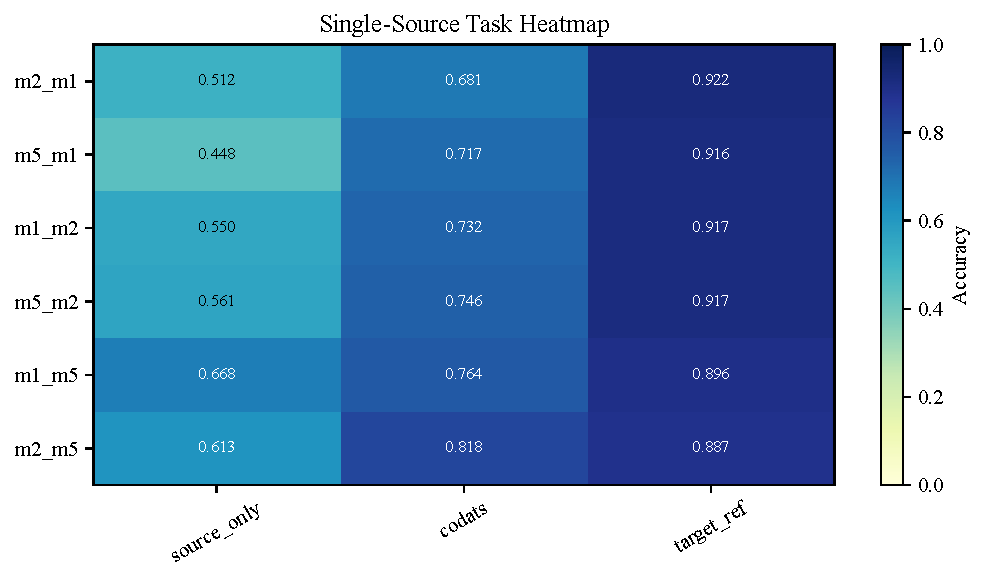
\includegraphics[width=1\textwidth]{figs/ch6_single_source_heatmap.pdf}
    \caption{单源跨工况8种方法逐任务目标域准确率热力图}
    \label{fig:single_source_heatmap}
\end{figure}

图 \ref{fig:single_source_mean_accuracy} 进一步以柱状图形式汇总单源任务的平均目标域准确率。该图与表 \ref{tab:single_average_results} 相互补充：柱状图便于观察方法间整体差距，表格则同时给出宏平均 F1、平衡准确率和无监督第一数。

\begin{figure}[!htbp]
    \centering
    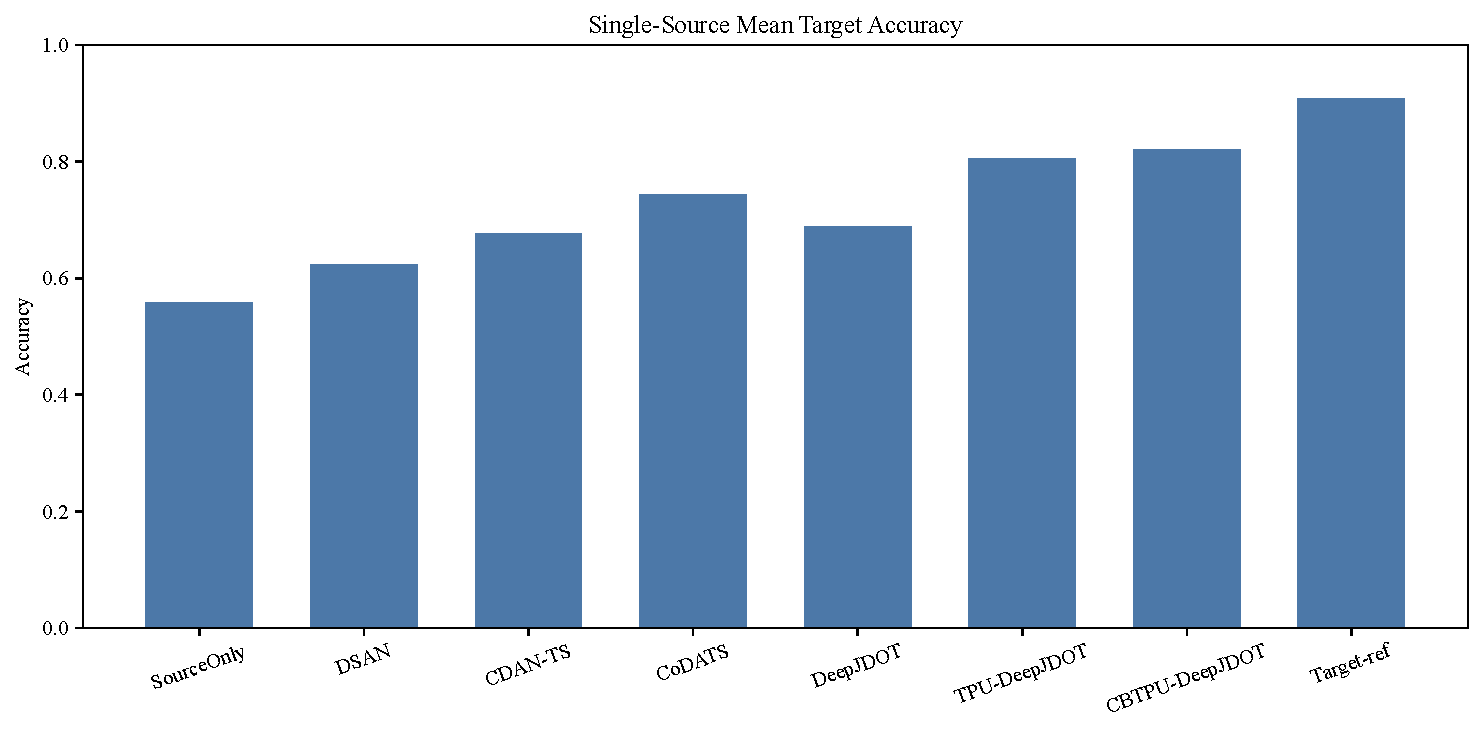
\includegraphics[width=0.92\textwidth]{figs/ch6_single_source_mean_accuracy.pdf}
    \caption{单源跨工况8种方法平均目标域准确率柱状图}
    \label{fig:single_source_mean_accuracy}
\end{figure}

表 \ref{tab:single_average_results} 给出单源跨工况实验的平均诊断性能。TPU-DeepJDOT 的平均准确率达到 80.54\%，相比 DeepJDOT 的 68.88\% 提升 11.66 个百分点，宏平均 F1 和平衡准确率分别提升 12.78 和 11.56 个百分点。CBTPU-DeepJDOT 的平均准确率进一步达到 82.02\%，相较 TPU-DeepJDOT 继续提升 1.48 个百分点，并在 6 个单源迁移方向上均取得无监督方法第一。该结果说明，第三章方法贡献了主要性能跃升，第四章方法在可靠对齐基础上进一步稳定细化目标域决策边界。

\begin{table}[!htbp]
    \centering
    \caption{单源跨工况主结果的平均诊断性能}
    \label{tab:single_average_results}
    \zihao{5}
    \setlength{\tabcolsep}{3pt}
    \begin{tabular}{@{}>{\raggedright\arraybackslash}p{0.24\textwidth}
                    >{\centering\arraybackslash}p{0.18\textwidth}
                    >{\centering\arraybackslash}p{0.18\textwidth}
                    >{\centering\arraybackslash}p{0.18\textwidth}
                    >{\centering\arraybackslash}p{0.16\textwidth}@{}}
        \toprule
        方法 & 准确率 & 宏平均 F1 & 平衡准确率 & 无监督第一数 \\
        \midrule
        SourceOnly & 55.88$\pm$7.67 & 49.97$\pm$7.96 & 55.83$\pm$7.79 & 0/6 \\
        DSAN & 62.42$\pm$13.35 & 58.45$\pm$15.51 & 62.41$\pm$13.67 & 0/6 \\
        CDAN-TS & 67.76$\pm$9.99 & 64.25$\pm$11.51 & 67.61$\pm$9.91 & 0/6 \\
        CoDATS & 74.30$\pm$4.62 & 72.34$\pm$5.72 & 74.33$\pm$4.71 & 0/6 \\
        DeepJDOT & 68.88$\pm$1.76 & 66.04$\pm$1.46 & 69.08$\pm$1.62 & 0/6 \\
        TPU-DeepJDOT & 80.54$\pm$2.20 & 78.82$\pm$2.18 & 80.64$\pm$2.28 & 0/6 \\
        CBTPU-DeepJDOT & 82.02$\pm$1.64 & 80.73$\pm$1.54 & 82.12$\pm$1.71 & 6/6 \\
        Target-ref & 90.92$\pm$1.42 & 90.67$\pm$1.66 & 90.98$\pm$1.41 & -- \\
        \bottomrule
    \end{tabular}
\end{table}

从单源热力图、平均柱状图和平均表可以得到两点结论。第一，单源方法符合 SourceOnly $<$ DeepJDOT $<$ TPU-DeepJDOT $<$ CBTPU-DeepJDOT 的总体趋势，说明本文方法并非只在单个代表任务上有效。第二，CBTPU-DeepJDOT 在 6/6 任务中均为无监督方法第一，说明多证据置信均衡伪标签学习的增益虽然幅度相对较小，但跨迁移方向具有一致性。

\subsection{多源创新方法相对基线方法的优势分析}

图 \ref{fig:two_source_heatmap} 给出 3 个两源域跨工况任务上的逐任务准确率热力图。该图用于观察源域数量较少时，不同方法在目标生产模式变化下的稳定性。SourceOnly 说明直接合并两个源域的有标签样本仍不足以消除跨工况偏移；CoDATS 能够提供一定领域对抗适配收益；WJDOT 引入逐源联合分布传输，但全局源域权重仍难以刻画类别级差异。CA-CCSR-WJDOT 在 3 个两源域跨工况任务中均取得无监督方法最高准确率，说明类条件源域可靠性加权在两源域跨工况场景下已经能够提供更稳定的选择性迁移。

\begin{figure}[!htbp]
    \centering
    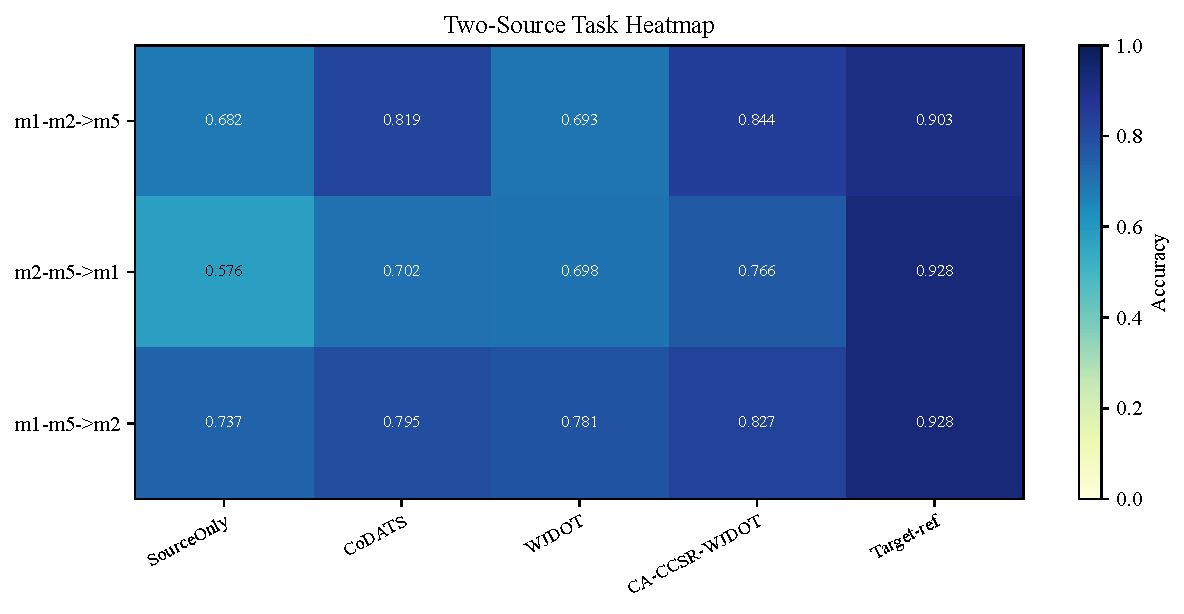
\includegraphics[width=0.92\textwidth]{figs/ch6_two_source_heatmap.pdf}
    \caption{两源域跨工况任务逐任务目标域准确率热力图}
    \label{fig:two_source_heatmap}
\end{figure}

图 \ref{fig:two_source_mean_accuracy} 给出两源域跨工况任务的平均目标域准确率柱状图。与逐任务热力图相比，该图更直观地呈现不同方法在两源域跨工况场景中的总体差距；完整指标仍以表 \ref{tab:two_source_average_results} 为准。

\begin{figure}[!htbp]
    \centering
    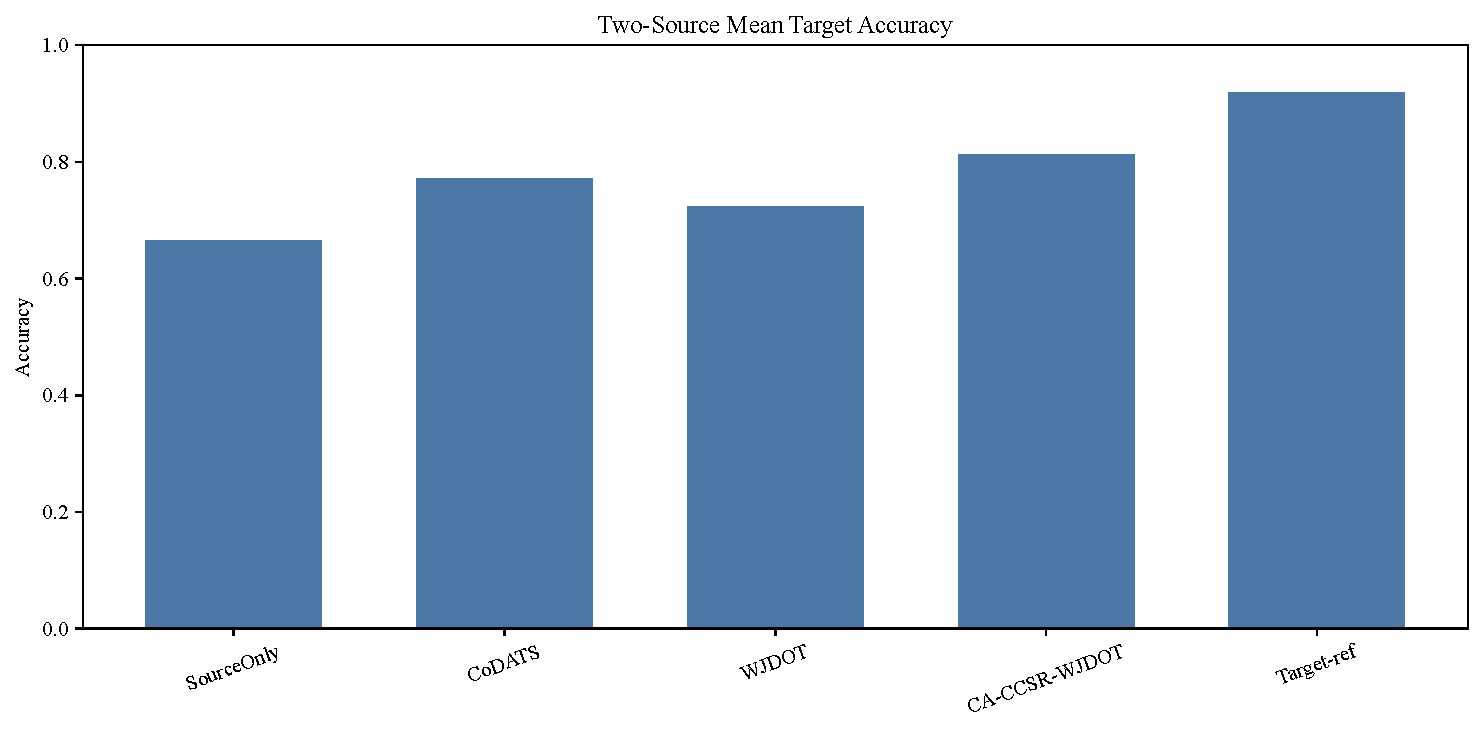
\includegraphics[width=0.86\textwidth]{figs/ch6_two_source_mean_accuracy.pdf}
    \caption{两源域跨工况任务平均目标域准确率柱状图}
    \label{fig:two_source_mean_accuracy}
\end{figure}

表 \ref{tab:two_source_average_results} 给出两源域跨工况任务的平均诊断性能。CA-CCSR-WJDOT 在 3 个两源域跨工况任务上均取得无监督方法第一，平均准确率达到 81.21\%，分别高于 CoDATS 和 WJDOT 3.99 和 8.80 个百分点。

\begin{table}[!htbp]
    \centering
    \caption{两源域跨工况主结果的平均诊断性能}
    \label{tab:two_source_average_results}
    \zihao{5}
    \setlength{\tabcolsep}{3pt}
    \begin{tabular}{@{}>{\raggedright\arraybackslash}p{0.24\textwidth}
                    >{\centering\arraybackslash}p{0.18\textwidth}
                    >{\centering\arraybackslash}p{0.18\textwidth}
                    >{\centering\arraybackslash}p{0.18\textwidth}
                    >{\centering\arraybackslash}p{0.16\textwidth}@{}}
        \toprule
        方法 & 准确率 & 宏平均 F1 & 平衡准确率 & 无监督第一数 \\
        \midrule
        SourceOnly & 66.51$\pm$8.20 & 62.00$\pm$7.06 & 66.58$\pm$8.21 & 0/3 \\
        CoDATS & 77.22$\pm$6.22 & 75.58$\pm$6.95 & 77.28$\pm$6.28 & 0/3 \\
        WJDOT & 72.41$\pm$4.96 & 69.07$\pm$5.40 & 72.50$\pm$4.96 & 0/3 \\
        CA-CCSR-WJDOT & 81.21$\pm$4.12 & 79.97$\pm$4.50 & 81.32$\pm$4.20 & 3/3 \\
        Target-ref & 91.94$\pm$1.44 & 91.49$\pm$0.92 & 91.98$\pm$1.42 & -- \\
        \bottomrule
    \end{tabular}
\end{table}

图 \ref{fig:five_source_heatmap} 给出 6 个五源域跨工况任务上的逐任务准确率热力图。五源域跨工况设置覆盖所有目标生产模式，能够更全面地检验多源可靠性建模在源域数量增加后的稳定性。CA-CCSR-WJDOT 在 6 个五源域跨工况任务中均取得无监督方法最高准确率，说明其收益并非依赖单一目标域，而是能够在不同目标生产模式下保持较稳定的多源选择性迁移效果。

\begin{figure}[!htbp]
    \centering
    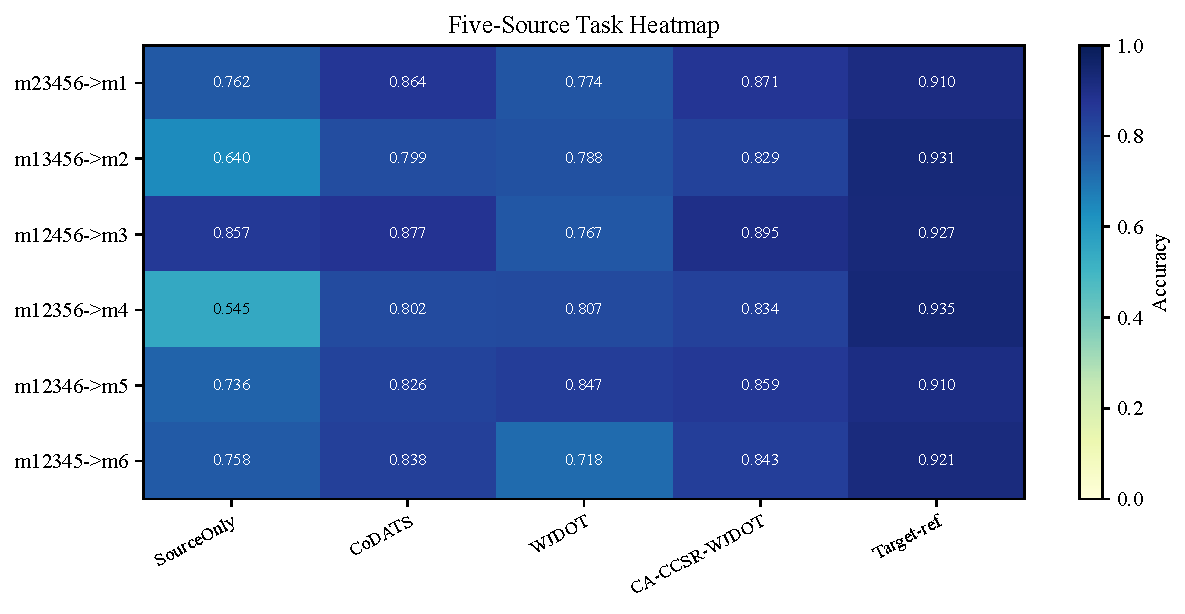
\includegraphics[width=0.92\textwidth]{figs/ch6_five_source_heatmap.pdf}
    \caption{五源域跨工况任务逐任务目标域准确率热力图}
    \label{fig:five_source_heatmap}
\end{figure}

图 \ref{fig:five_source_mean_accuracy} 给出五源域跨工况任务的平均目标域准确率柱状图。该图显示 CA-CCSR-WJDOT 在五源域跨工况场景下整体高于 CoDATS 和 WJDOT；表 \ref{tab:multi_average_results} 进一步给出宏平均 F1、平衡准确率和无监督第一数。

\begin{figure}[!htbp]
    \centering
    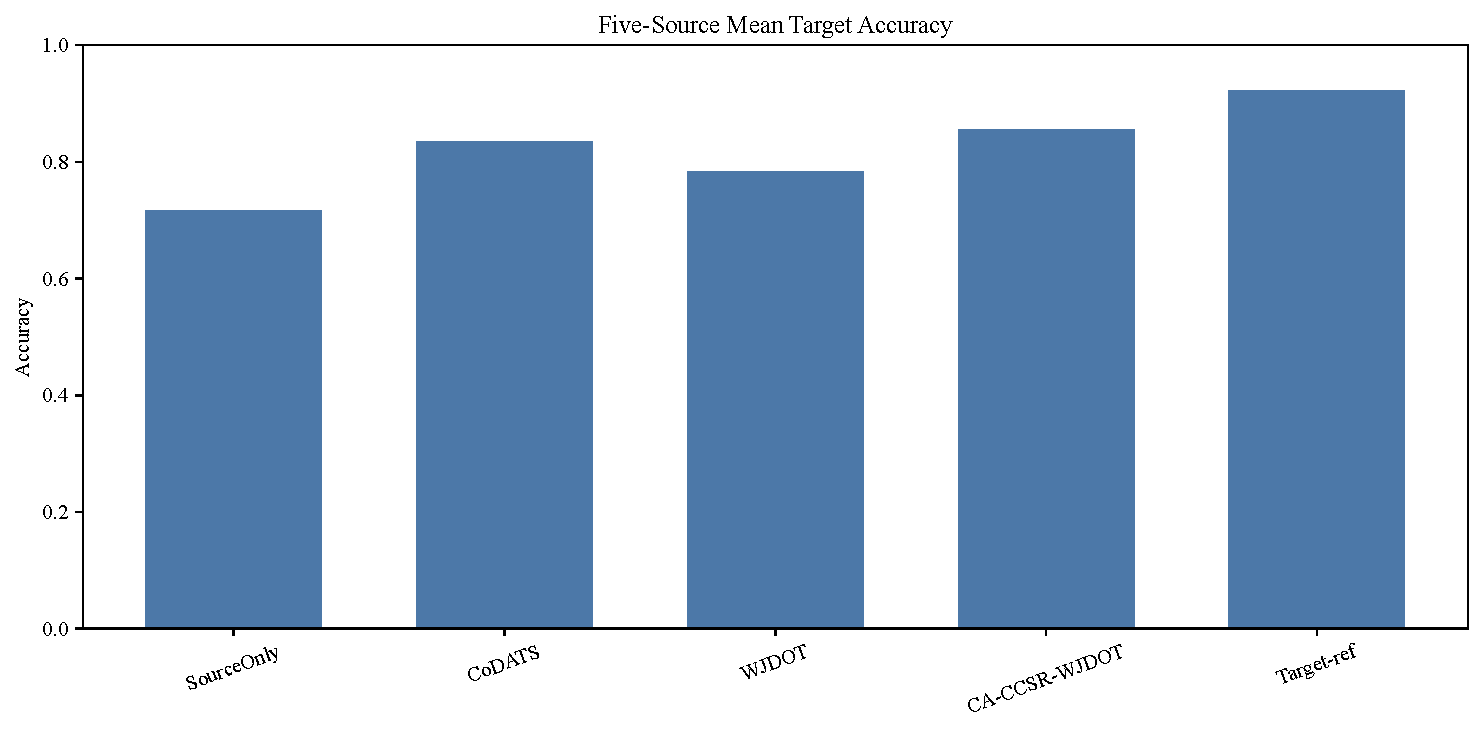
\includegraphics[width=0.86\textwidth]{figs/ch6_five_source_mean_accuracy.pdf}
    \caption{五源域跨工况任务平均目标域准确率柱状图}
    \label{fig:five_source_mean_accuracy}
\end{figure}

表 \ref{tab:multi_average_results} 给出五源域跨工况任务的平均诊断性能。CA-CCSR-WJDOT 在 6 个目标生产模式上均取得无监督方法第一，平均准确率达到 85.50\%，高于 CoDATS 的 83.44\% 和 WJDOT 的 78.37\%。宏平均 F1 和平衡准确率也呈现相同趋势，说明该方法的收益并非只来自样本数量较多的类别。

\begin{table}[!htbp]
    \centering
    \caption{五源域跨工况主结果的平均诊断性能}
    \label{tab:multi_average_results}
    \zihao{5}
    \setlength{\tabcolsep}{3pt}
    \begin{tabular}{@{}>{\raggedright\arraybackslash}p{0.24\textwidth}
                    >{\centering\arraybackslash}p{0.18\textwidth}
                    >{\centering\arraybackslash}p{0.18\textwidth}
                    >{\centering\arraybackslash}p{0.18\textwidth}
                    >{\centering\arraybackslash}p{0.16\textwidth}@{}}
        \toprule
        方法 & 准确率 & 宏平均 F1 & 平衡准确率 & 无监督第一数 \\
        \midrule
        SourceOnly & 71.63$\pm$10.88 & 68.04$\pm$12.61 & 71.48$\pm$11.15 & 0/6 \\
        CoDATS & 83.44$\pm$3.19 & 82.46$\pm$3.42 & 83.21$\pm$3.53 & 0/6 \\
        WJDOT & 78.37$\pm$4.30 & 75.70$\pm$5.30 & 78.47$\pm$4.35 & 0/6 \\
        CA-CCSR-WJDOT & 85.50$\pm$2.50 & 84.30$\pm$2.58 & 85.51$\pm$2.54 & 6/6 \\
        Target-ref & 92.24$\pm$1.07 & 91.46$\pm$1.21 & 92.28$\pm$1.09 & -- \\
        \bottomrule
    \end{tabular}
\end{table}

为解释五源域跨工况热力图中的稳定优势，图 \ref{fig:class_source_alpha_heatmap} 以第 6.3.3 节的五源域代表任务为例，给出 CA-CCSR-WJDOT 的源域--类别权重。不同故障类别并不依赖同一个源域：部分类别更偏向 $m_1$，部分类别更偏向 $m_4$ 或 $m_6$，也有若干类别由多个源域共同提供信息。该结果说明，方法的优势不是简单平均多个源域，而是在“源域--故障类别”层面重新分配迁移贡献。

\begin{figure}[!htbp]
    \centering
    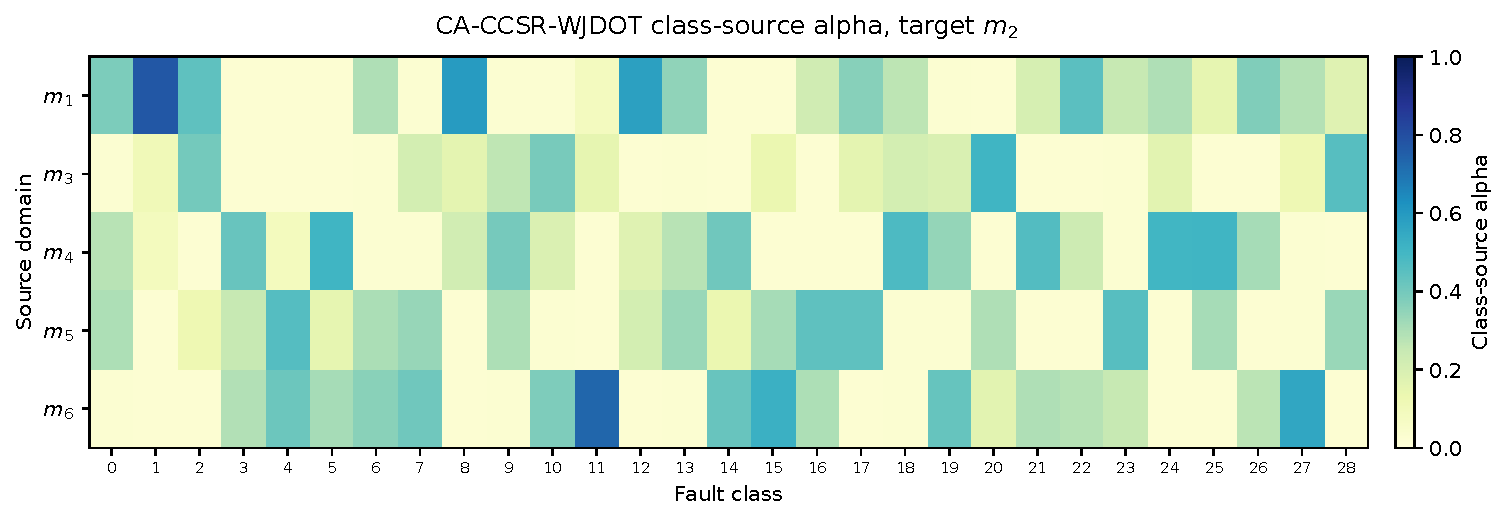
\includegraphics[width=0.92\textwidth]{figs/ch6_class_source_alpha_heatmap.pdf}
    \caption{五源域跨工况任务 $\{m_1,m_3,m_4,m_5,m_6\}\rightarrow m_2$ 中 CA-CCSR-WJDOT 的源域--类别权重热力图}
    \label{fig:class_source_alpha_heatmap}
\end{figure}

为验证方法提升是否具有跨迁移场景的一致性，本文采用 Wilcoxon signed-rank test 对相邻方法进行配对检验。这里的配对单位是迁移场景，而不是多随机种子重复实验，因此检验结论表述为“跨迁移场景配对显著性”。检验结果如表 \ref{tab:significance_results} 所示，三组相邻方法比较均呈现跨场景一致正向差异。

\begin{table}[!htbp]
    \centering
    \caption{相邻方法跨迁移场景配对显著性检验结果}
    \label{tab:significance_results}
    \zihao{5}
    \setlength{\tabcolsep}{3pt}
    \begin{tabular}{@{}>{\raggedright\arraybackslash}p{0.37\textwidth}
                    >{\centering\arraybackslash}p{0.20\textwidth}
                    >{\centering\arraybackslash}p{0.17\textwidth}
                    >{\centering\arraybackslash}p{0.20\textwidth}@{}}
        \toprule
        配对比较 & 配对场景 & 正向场景数 & Wilcoxon $p$ 值 \\
        \midrule
        TPU-DeepJDOT vs. DeepJDOT & 单源6任务 & 6/6 & 0.015625 \\
        CBTPU-DeepJDOT vs. TPU-$\sim$ & 单源6任务 & 6/6 & 0.015625 \\
        CA-CCSR-WJDOT vs. WJDOT & 多源共9任务 & 9/9 & 0.001953 \\
        \bottomrule
    \end{tabular}
\end{table}

\section{本章小结}

本章围绕田纳西伊斯曼过程领域自适应数据集，在统一实验协议下对单源和多源跨工况故障诊断方法进行了实验验证。单源实验表明，TPU-DeepJDOT 相比 DeepJDOT 明显提升平均准确率、宏平均 F1 和平衡准确率，验证了时序原型非平衡联合分布对齐的有效性；CBTPU-DeepJDOT 相比 TPU-DeepJDOT 进一步取得一致增益，并在 6/6 个单源任务中取得无监督方法第一，验证了多证据置信均衡伪标签机制的作用。

多源实验表明，CA-CCSR-WJDOT 在两源域跨工况设置中 3/3 第一，在五源域跨工况设置中 6/6 第一，并在五源域跨工况任务上达到 85.50$\pm$2.50\% 的平均准确率，整体优于 CoDATS 和 WJDOT。该结果说明，类条件源域可靠性加权能够缓解 WJDOT 全局源域权重粒度过粗的问题，并提升多源选择性迁移能力。

总体而言，本章按照方法递进关系组织实验叙事，正文保留单源主结果表、单源逐任务热力图、单源平均柱状图、两源和五源多源主结果表、两源和五源逐任务热力图、两源和五源平均柱状图、代表场景混淆矩阵与特征可视化、源域--类别权重热力图以及显著性检验表。实验结果共同说明，本文方法能够在目标域无标签条件下提升工业过程跨工况故障诊断性能，并为源域可靠性差异提供必要解释。

\chapter{总结与展望}

\section{工作总结}

本文围绕工业过程跨工况故障诊断中的领域分布偏移、目标域标签不足以及多源负迁移等问题，开展基于领域自适应的故障诊断方法研究。以田纳西伊斯曼过程领域自适应数据集为实验对象，本文分别从单源域到单目标域和多源域到单目标域两类场景出发，研究联合分布最优传输、时序原型约束、置信均衡伪标签学习以及类条件源域可靠性加权等方法在工业过程故障诊断中的应用。

在单源场景中，本文以深度联合分布最优传输方法为基础，针对普通平衡最优传输可能导致错误强制匹配、且原始联合传输过程缺少工业时间序列故障结构约束的问题，提出时序原型非平衡联合分布对齐方法。该方法通过非平衡最优传输降低不可靠源目标样本被强制匹配的风险，并结合源域类别原型、时间序列统计代价和源域监督对比学习增强故障类别结构表达能力。针对目标域无标签条件下伪标签可靠性不足的问题，进一步提出多证据置信均衡伪标签方法。该方法综合传输计划、教师模型预测和源域原型距离三类语义证据，对目标域样本进行一致性筛选，并通过动态置信阈值、类别均衡机制和强弱增强一致性约束，提高目标域无标签样本利用的可靠性。

在多源场景中，本文以多源加权联合分布最优传输为基础，考虑到不同源域与目标域之间存在差异，且同一源域对不同故障类别的贡献并不一致，提出类条件源域可靠性加权方法。该方法结合卷积式时间序列领域自适应表征、逐源联合分布最优传输和源域--故障类别可靠性矩阵，对不同源域在不同故障类别上的迁移贡献进行建模，从而形成更细粒度的多源选择性迁移机制。同时，在多源方法中引入领域对抗特征约束与教师先验保护机制，以增强时序表征能力，并降低新增迁移损失破坏已有表征的风险。

实验部分围绕单源跨工况和多源跨工况两类任务展开。本文采用诊断准确率、宏平均 F1 值、平衡准确率、混淆矩阵和跨域特征可视化等指标，对所提方法与源域直接迁移、典型领域自适应方法、DeepJDOT、WJDOT、CoDATS 以及目标域监督参考方法进行对比分析，并通过关键机制对比、典型场景分析和可解释性分析讨论时序原型约束、非平衡传输、多证据伪标签筛选、类别均衡机制以及类条件源域可靠性矩阵等设计的作用。考虑到不同跨工况任务的分布偏移程度和源域可靠性差异并不一致，结果分析重点关注整体趋势、典型成功场景和局部失效场景，避免将单一场景结果解释为绝对优势。整体而言，本文方法在跨工况故障诊断任务中表现出一定适应能力和解释价值，可为工业过程故障诊断中的无监督领域自适应研究提供方法参考。

\subsection{本文主要研究内容}

本文的主要研究内容可以概括为以下三个方面。

第一，研究单源跨工况故障诊断中的时序原型非平衡联合分布对齐方法。针对深度联合分布最优传输方法在小批量训练中可能存在的错误强制匹配问题，引入非平衡传输思想，对源域与目标域样本之间的传输约束进行松弛，使不可靠匹配能够被弱化。同时，考虑到工业过程样本为多变量时间序列，构造源域故障类别原型和时间序列统计代价，用于增强跨工况对齐过程中的故障类别结构保持能力。为提高源域类别原型的稳定性，进一步加入源域监督对比学习，使特征空间中的同类故障样本更加紧凑、异类故障样本更加分离。

第二，研究单源跨工况故障诊断中的多证据置信均衡伪标签学习方法。针对目标域无标签样本难以直接利用、伪标签易受噪声影响的问题，未直接采用分类器置信度作为唯一依据，而是从传输计划、教师模型预测和源域原型距离三个角度构建目标样本的多证据语义分布。只有当多种证据在类别判断上具有较高一致性且满足动态置信阈值要求时，目标样本才被纳入伪标签学习过程。同时，在可信伪标签集合上估计类别频率，并结合类别均衡和强弱增强一致性约束，缓解目标伪标签类别偏置和过拟合风险。

第三，研究多源跨工况故障诊断中的类条件源域可靠性加权方法。针对多源数据简单合并可能掩盖源域差异、全局源域权重难以表达类别级迁移可靠性的问题，构建源域--故障类别可靠性矩阵。该矩阵综合考虑源域类别原型距离、类内传输代价、目标预测不确定性和源域类别性能等因素，用于度量不同源域在不同故障类别上的迁移可靠性。在此基础上，将 CoDATS 的卷积式时间序列表征能力、WJDOT 的逐源联合传输思想和 CCSR 的类条件源域加权机制结合起来，以提升多源跨工况故障诊断的选择性迁移能力和可解释性。

\subsection{本文主要创新点}

本文的主要创新点如下。

（1）提出了一种基于时序原型非平衡联合分布对齐的单源领域自适应故障诊断方法。该方法在深度联合分布最优传输基础上，引入非平衡最优传输机制，以缓解小批量训练中目标样本被错误源样本强制匹配的问题；同时利用源域类别原型和时间序列统计代价刻画工业故障的类别结构与动态响应特征，并通过源域监督对比学习增强特征空间的类别可分性。该方法将单源领域自适应故障诊断从样本级联合分布对齐扩展到带有时序类别结构约束的选择性对齐。

（2）提出了一种基于多证据置信均衡伪标签的单源领域自适应故障诊断方法。该方法针对目标域伪标签不可靠问题，综合利用传输语义分布、教师预测语义分布和源域原型语义分布三类证据，对目标域样本进行一致性筛选。与仅依赖分类器最大置信度的伪标签方法不同，该方法通过多证据一致性机制降低单一预测源过置信带来的错误传播风险，并结合动态置信阈值、类别均衡和强弱增强一致性约束，提高目标域无标签样本利用过程的稳定性。

（3）提出了一种基于类条件源域可靠性加权的多源领域自适应故障诊断方法。该方法针对多源跨工况场景中的源域负迁移问题，将源域整体权重细化为源域--故障类别层面的可靠性权重，用于刻画不同源域对不同故障类别的迁移贡献。在模型设计上，本文结合卷积式时间序列表征、领域对抗特征约束、逐源联合分布最优传输和教师先验保护机制，使多源迁移过程既能够利用强时序表征，又能够通过类条件源域可靠性矩阵进行可解释的源类选择。

\subsection{存在不足}

尽管本文围绕跨工况领域自适应故障诊断提出了多种改良方法，并在田纳西伊斯曼过程数据集上进行了实验验证，但仍存在以下不足。

第一，部分跨工况任务中源域与目标域差异较大，模型性能提升幅度仍然有限。特别是在目标模式与源模式之间分布差异明显时，源域类别原型、传输计划和教师预测都可能受到偏移影响，导致目标域伪语义估计不够稳定。虽然本文通过非平衡传输、多证据筛选和教师先验保护等机制降低了错误迁移风险，但在更强分布偏移场景下仍可能出现适配不足或负迁移现象。

第二，本文方法包含多个相互作用的机制，模型复杂度和训练成本相对较高。与源域直接迁移或简单领域对抗方法相比，本文方法需要计算最优传输代价、更新源域类别原型、估计多证据伪标签以及构建源域--类别可靠性矩阵。这些步骤提升了方法的表达能力和可解释性，但也增加了训练时间和方法复杂度。面向计算效率受限或大规模实验设定时，仍需进一步研究如何在保持诊断性能的同时降低计算开销。

第三，目标域无标签条件下的模型选择仍然是一个困难问题。本文在训练过程中避免使用目标域评估标签，并采用源域验证性能、目标预测熵、类别分布稳定性和教师先验等无标签指标辅助模型选择。然而，这些指标只能间接反映目标域性能，不能完全替代真实目标域标签监督。当目标域分布偏移较大或预测分布发生坍缩时，无标签模型选择策略仍可能存在偏差。

第四，本文的多源可靠性建模主要依赖特征距离、传输代价、预测不确定性和源域类别性能等统计量。这些指标能够反映一定的源域--类别可靠性差异，但仍属于经验性度量，对不同数据集、不同故障类型和不同模型结构的泛化能力有待进一步验证。此外，类条件源域可靠性矩阵能够提供一定解释性，但解释粒度主要停留在源域和故障类别层面，尚未深入到具体传感器变量、物理过程环节和故障传播机理层面。

第五，本文实验主要基于田纳西伊斯曼过程领域自适应数据集展开。该数据集具有代表性的多模式化工过程特点，适合验证跨工况领域自适应方法，但其仍属于仿真基准数据。若进一步拓展到噪声机制更复杂、缺失模式更多、故障类型开放或工况连续变化的数据设定，本文方法的泛化规律仍需系统分析。

\section{未来展望}

针对本文工作仍存在的不足，未来可从以下几个方向继续开展研究。

第一，研究弱监督目标域校准方法。本文主要关注无监督领域自适应场景，即训练过程中不使用目标域标签。然而，在弱监督设定中，完全无标签和完全有标签之间还存在多种中间形式，例如仅有少量目标域标签、部分故障标签不完整、标签存在噪声或只能获得粗粒度类别约束。未来可以考虑将少量可靠目标标签用于校准类别原型、源域可靠性矩阵或伪标签阈值，而不是直接进行目标域监督训练。这样既可以保持领域自适应方法对标签稀缺场景的适用性，又能利用少量先验信息提高目标伪标签和源类可靠性估计的准确性。

第二，研究在线测试时领域自适应方法。本文采用离线领域自适应设置，即训练阶段可以访问一批无标签目标域数据。当目标域样本按时间顺序到达且目标分布持续演化时，可以进一步研究在线测试时自适应方法，使模型能够在推理过程中根据新到达的无标签样本持续更新自身状态\cite{wang2022cotta}。同时，需要避免在线自适应过程中因错误伪标签导致的误差累积和灾难性遗忘问题，并约束在线更新幅度、推断复杂度和预测稳定性。

第三，研究更具可解释性的领域自适应故障诊断方法。本文通过源域--故障类别可靠性矩阵展示了不同源域对不同故障类别的贡献差异，但解释粒度仍然有限。未来可以进一步结合注意力机制、特征归因、因果分析和过程机理知识，分析哪些传感器变量、哪些时间片段以及哪些物理过程环节对跨工况迁移起关键作用。对于化工过程故障诊断而言，将领域自适应结果与反应器、冷凝器、分离器、压缩机等过程单元结构联系起来，有助于增强解释结果与过程机理的一致性。

第四，研究面向计算效率约束的轻量化领域自适应模型。本文方法包含最优传输、原型更新、教师模型和多源可靠性估计等步骤，计算成本相对较高。未来可以通过模型剪枝、知识蒸馏、低秩近似、量化推理和轻量化时序网络设计降低模型复杂度。同时，可以进一步研究小批量最优传输的高效近似算法，以分析模型规模、推断复杂度和诊断性能之间的关系。

第五，研究更加鲁棒的多源选择与负迁移抑制机制。本文从源域--类别层面对多源可靠性进行建模，但当源域数量进一步增加、源域质量差异更大或目标工况显著偏离所有已有源工况时，现有可靠性矩阵可能仍不足以完全避免负迁移。未来可以引入不确定性估计、贝叶斯源域选择、元学习校准或因果不变特征学习，对源域可迁移性进行更稳健的判断。同时，也可以研究源域自动筛选机制，使模型在发现某些源域与目标域关系较弱时，能够主动降低其参与训练和推理的权重。

第六，研究面向开放故障和未知工况的领域自适应诊断方法。本文默认源域和目标域具有相同故障类别空间，属于闭集领域自适应设置。但在开放诊断设定中，目标域可能包含训练集中未出现的新故障类型，也可能对应新的生产模式和未知扰动。未来可以扩展到开放集领域自适应、部分领域自适应和通用领域自适应等更复杂设置，使模型不仅能够识别已知故障，还能够发现未知故障或拒识不确定样本，从而增强跨工况诊断模型的开放集识别能力。

综上，本文为跨工况工业过程故障诊断提供了基于最优传输、时序原型、置信伪标签和类条件源域可靠性的领域自适应方法框架。后续若进一步结合弱监督目标校准、在线自适应、可解释建模和轻量化方法，有望提升模型在复杂跨域设定中的泛化能力、稳定性和研究价值。

\cleardoublepage
\bibliography{bib/references}

\clearpage
\appendix
\renewcommand{\thetable}{\Alph{chapter}.\arabic{table}}
\chapter{论文符号表}

为避免正文中同一符号表示不同含义，本文将主要数学符号统一整理如表 \ref{tab:symbols} 所示。上标 $s$、$t$ 和 $s_k$ 分别表示源域、目标域和第 $k$ 个源域；未列入表中的局部求和下标仅在其所在公式附近使用。

{\zihao{5}
\setlength{\tabcolsep}{3.5pt}
\renewcommand{\arraystretch}{1.18}
\setlength{\emergencystretch}{3em}
\hbadness=10000
\hfuzz=40pt
\vbadness=10000
\begin{longtable}{@{}>{\raggedright\arraybackslash}p{0.30\textwidth}>{\raggedright\arraybackslash}p{0.42\textwidth}>{\raggedright\arraybackslash}p{0.22\textwidth}@{}}
    \caption{论文主要符号表}
    \label{tab:symbols}\\
    \toprule
    符号 & 含义 & 说明 \\
    \midrule
    \endfirsthead
    \multicolumn{3}{r}{续表~\thetable}\\
    \toprule
    符号 & 含义 & 说明 \\
    \midrule
    \endhead
    \bottomrule
    \endfoot
    \bottomrule
    \endlastfoot

    \multicolumn{3}{l}{\textbf{数据、领域与类别}}\\
    \addlinespace
    $\mathcal{D}_s,\mathcal{D}_t,\mathcal{D}_{s_k}$ & 源域、目标域、第 $k$ 个源域数据集 & 单源或多源领域自适应设定 \\
    $\mathcal{D}_{s}^{\mathrm{train}}$、$\mathcal{D}_{t}^{\mathrm{train}}$、$\mathcal{D}_{t}^{\mathrm{test}}$ & 源域训练集、目标域无标签训练集、目标域测试集 & 目标域测试标签仅用于最终评价 \\
    $\mathcal{B}_s,\mathcal{B}_t,\mathcal{B}_{s_k}$ & 源域小批量、目标域小批量、第 $k$ 个源域小批量 & 训练迭代中采样得到 \\
    $\mathcal{B}_s^c$ & 源域小批量中第 $c$ 类样本集合 & 用于源域原型更新 \\
    $x,x_i^s,x_j^t,x_i^{s_k},x_u^t$ & 通用样本、源域样本、目标域样本、第 $k$ 源域样本、目标测试样本 & 均表示多变量时间序列窗口 \\
    $y_i^s,y_i^{s_k},y_u^t$ & 源域标签、第 $k$ 源域标签、目标域测试标签 & $y_u^t$ 不参与训练 \\
    $h$ & 目标域诊断函数 & 由训练后的诊断模型给出 \\
    $P_s(X)$、$P_t(X)$、$P_{s_k}(X)$、$P_{s_l}(X)$ & 源域、目标域及不同源域的数据分布 & 用于描述分布偏移 \\
    $\mathbf{X}^{(m)}$ & 第 $m$ 个生产模式的数据张量 & 维度为 $N_m\times600\times34$ \\
    $V,L,L'$ & 过程变量数量、输入时间窗口长度、卷积输出时间长度 & $L'$ 仅用于全局平均池化 \\
    $n_s,n_t,n_k,N_m$ & 源域样本数、目标域样本数、第 $k$ 源域样本数、第 $m$ 模式样本数 & 数据集规模 \\
    $n_s^{\mathrm{bat}},n_t^{\mathrm{bat}}$ & 源域小批量大小与目标域小批量大小 & 非平衡传输公式中的批量维度 \\
    $K,N_c$ & 源域数量、故障类别数量 & TEP 数据集中 $N_c=29$ \\
    $\mathcal{Y}$ & 标签空间 & $\{0,1,\cdots,28\}$ \\
    $m_1,\cdots,m_6$ & TEP 生产模式编号 & 实验场景中的领域标识 \\
    $m_s,m_t,m_{s_1},\cdots,m_{s_K}$ & 源模式、目标模式、多个源模式 & 用于迁移任务表示 \\
    $x_{i,t,j}^{(m)},\tilde{x}_{i,t,j}^{(m)}$ & 原始样本取值与标准化后取值 & 第 $m$ 模式、第 $i$ 样本、第 $t$ 时间步、第 $j$ 变量 \\
    $\bar{x}_{j}^{(m)},\sigma_{j}^{(m)}$ & 第 $m$ 模式第 $j$ 个变量的均值与标准差 & 用于模式内标准化 \\
    $\epsilon$ & 数值稳定常数 & 防止除零或对数为零 \\
    $\nu,N_{\mathrm{iter}}$ & 训练步索引与总训练步数 & $\nu$ 不再表示时间序列下标 \\

    \addlinespace
    \multicolumn{3}{l}{\textbf{模型、特征与预测}}\\
    \addlinespace
    $F_\theta(\cdot)$ & 特征提取器 & 参数为 $\theta$ \\
    $G_\phi(\cdot)$ & 故障分类器 & 参数为 $\phi$ \\
    $G_{\phi,c}(\cdot)$ & 分类器输出第 $c$ 类概率的分量 & 领域对抗基线公式中使用 \\
    $D_\omega(\cdot)$ & 领域判别器 & 参数为 $\omega$ \\
    $\Theta,\bar{\Theta},\Theta_{\mathrm{TPU}}$ & 学生模型、教师模型和 TPU-DeepJDOT 阶段模型参数集合 & $\Theta=(\theta,\phi)$，$\bar{\Theta}=(\bar{\theta},\bar{\phi})$ \\
    $\xi$ & 指数滑动平均教师衰减系数 & 仅在滑动平均教师形式下用于更新 $\bar{\Theta}$ \\
    $z,z_i^s,z_j^t,z_i^{s_k},\tilde{z}_i$ & 深度特征、源特征、目标特征、多源特征、归一化特征 & 由 $F_\theta$ 输出或归一化得到 \\
    $d_z,d_\psi$ & 深度特征维度与时序描述符维度 & 用于代价归一化 \\
    $p,p_i^{s_k},p_j^t,p_{kj}^t,p_{kjr}^t,p_{jc}$ & 类别预测概率分布及其分量 & $p_{kjr}^t$ 和 $p_{jc}$ 表示对应类别分量 \\
    $p_{\theta,\phi}(\cdot|x)$ & 学生模型对样本 $x$ 的 softmax 概率 & 等价于 $G_\phi(F_\theta(x))$ 的概率输出 \\
    $p_j^{\mathrm{stu}},p_j^{\mathrm{tea}},p_j^{\mathrm{final}}$ & 学生预测、教师预测和最终融合预测概率 & 教师--学生预测融合使用 \\
    $s_j^{\mathrm{stu}},s_j^{\mathrm{tea}},\Delta_{\mathrm{conf}},\Delta_{\min},\Delta_{\max},\omega_{\mathrm{mix}}$ & 学生/教师置信度与融合参数 & 第四章教师--学生预测融合使用 \\
    $p_j^{\mathrm{base}}$、$p_j^{\mathrm{pb}}$、$\bar{p}^{\mathrm{base}}$ & 基础混合预测、先验均衡预测、批次平均预测 & 无标签概率校正使用 \\
    $\hat{y},\hat{y}_j^t$ & 预测类别或伪标签类别 & 由概率分布的最大分量确定 \\
    $u_{jc},\tilde{u}_{jc},\tilde{u}_j$ & 原始预测得分、类别均衡后得分及其向量形式 & 伪标签类别均衡使用 \\
    $u_j^{\mathrm{tea}},u_j^{\mathrm{stu}}$ & 教师模型和学生模型的未归一化预测得分 & 教师先验约束使用 \\
    $a_w(\cdot),a_s(\cdot)$ & 弱增强与强增强变换 & 用于目标域一致性学习 \\
    $U^{(l-1)}$、$U^{(l)}$、$U$、$U_{r,t}$、$z_r$、$W^{(l)}$、$b^{(l)}$ & 卷积层输入/输出、最终卷积输出元素、池化后特征元素、卷积核与偏置 & 卷积式时间序列特征提取 \\
    $\varphi(\cdot)$ & 非线性激活函数 & 与标准差 $\sigma_{\cdot}$ 区分 \\
    $Z_s,Z_t$ & 源域特征集合与目标域特征集合 & 领域对抗损失中使用 \\

    \addlinespace
    \multicolumn{3}{l}{\textbf{最优传输与对齐}}\\
    \addlinespace
    $C,C_{ij},C_{ij}^{(k)},C^{(k)},C^{\mathrm{loss}}$ & 传输代价矩阵、代价元素、第 $k$ 源域代价、矩阵形式、训练代价 & $C$ 专用于代价矩阵 \\
    $\gamma$、$\gamma^\ast$、$\gamma_{ij}$、$\gamma_{ij}^{(k)}$、$\gamma_k$、$\gamma_k^\ast$、$\gamma_{k,ij}$ & 传输计划、最优传输计划及其元素、第 $k$ 源域传输计划及其元素 & 表示源目标样本匹配质量 \\
    $\Pi(a,b),\Pi(a_k,b)$ & 满足边际分布的传输计划集合 & $a_k$ 为第 $k$ 源域边际 \\
    $a,b,a_k$ & 源域边际、目标域边际、第 $k$ 源域边际 & 传输计划的边际质量 \\
    $\mathbf{1}$ & 全 1 向量 & 下标表示向量长度 \\
    $\varepsilon$ & 熵正则系数 & 非平衡 Sinkhorn 求解中使用 \\
    $\tau_s,\tau_t$ & 源边际与目标边际的松弛强度 & 仅用于非平衡最优传输 \\
    $\mathrm{KL}(\cdot\|\cdot),\langle\cdot,\cdot\rangle$ & KL 散度与矩阵内积 & 传输目标和一致性损失中使用 \\
    $\mathcal{L}_{\mathrm{UOT}}$ & 非平衡最优传输目标 & 用于说明非平衡传输原理 \\
    $c_{ij}^{f},c_{ij}^{y},c_{ij}^{\mathrm{temp}}$ & 特征代价、标签预测代价和时序统计代价 & 组成联合传输代价 \\
    $\operatorname{dist}(\cdot,\cdot)$ & 特征空间距离函数 & 避免与维度 $d_z$ 混淆 \\
    $\ell(\cdot,\cdot)$ & 分类或标签预测损失 & 通常为交叉熵 \\
    $\lambda_f,\lambda_y$ & 特征代价与标签代价权重 & 传输代价中的权重 \\
    $\lambda_{\mathrm{ot}},\lambda_{\mathrm{ot}}(\nu)$ & 最优传输对齐损失权重 & 后者表示随训练步变化的调度权重 \\
    $\lambda_p(\nu),\lambda_{\mathrm{temp}}(\nu),\lambda_p^0$ & 原型代价权重、时序统计代价权重、原型代价基础权重 & 延迟启动并线性预热 \\
    $\nu_p,S_p$ & 原型代价启动步数与预热步数 & 时序统计代价采用相同形式 \\

    \addlinespace
    \multicolumn{3}{l}{\textbf{原型、伪标签与一致性}}\\
    \addlinespace
    $\mu_c,\bar{\mu}_c,\mu_{kc}^s,\mu_c^t$ & 源域类别原型、小批量源类均值、第 $k$ 源域原型、目标域原型 & 用于类别结构建模 \\
    $\rho$ & 源域原型动量系数 & 原型指数滑动平均 \\
    $d_{cj}^{\mathrm{proto}},d_{jc}^{\mathrm{proto}}$ & 目标样本到源域类别原型的距离 & 分别服务于传输代价和原型语义分布 \\
    $\overline{d}_{-y_i^s,j}^{\mathrm{proto}}$、$\sigma_j^{\mathrm{proto}}$ & 目标样本到其他有效源类原型距离的均值与标准差 & 相对原型代价归一化 \\
    $r_{ij}^{\mathrm{proto}},r_{\min},r_{\max}$ & 相对原型代价及其裁剪下界和上界 & 衡量目标样本相对接近源类别的程度 \\
    $\bar{x}_{\mathrm{seq}}(x),\sigma_{\mathrm{seq}}(x)$ & 样本时间维度均值与标准差 & 时序描述符的一部分 \\
    $\bar{\Delta}_{\mathrm{seq}}(x),\sigma_{\Delta}(x)$ & 一阶差分均值与标准差 & 时序描述符的一部分 \\
    $\Delta x_{:,t}$ & 样本在时间维度上的一阶差分 & 时序描述符的一部分 \\
    $\psi(x)$ & 时间序列统计描述符 & 由均值、标准差和一阶差分统计量拼接得到 \\
    $\mathcal{P}(i),\mathcal{I}$ & 样本 $i$ 的同类正样本集合、存在正样本的索引集合 & 源域监督对比学习 \\
    $T_{\mathrm{con}}$ & 监督对比学习温度 & 与可靠性和蒸馏温度区分 \\
    $q_j^{\mathrm{ot}}$、$q_j^{\mathrm{cls}}$、$q_j^{\mathrm{proto}}$、$q_j^{\mathrm{mix}}$ & 传输语义、教师预测语义、原型语义和融合语义分布 & 多证据伪标签筛选 \\
    $m_{cj}^{\mathrm{ot}}$ & 第 $c$ 类源样本传向目标样本 $j$ 的传输质量 & 归一化后得到 $q_j^{\mathrm{ot}}$ \\
    $\hat{y}_j^{\mathrm{ot}}$、$\hat{y}_j^{\mathrm{cls}}$、$\hat{y}_j^{\mathrm{proto}}$ & 三类语义证据各自的最大概率类别 & 多证据一致性判断使用 \\
    $\kappa_j$ & 目标样本融合语义置信度 & $\kappa_j=\max_c q_{jc}^{\mathrm{mix}}$ \\
    $\alpha_{\mathrm{ot}}$、$\alpha_{\mathrm{cls}}$、$\alpha_{\mathrm{proto}}$ & 三类语义证据的融合指数 & 用于幂加权几何平均 \\
    $D_{\mathrm{JS}},\bar{q},\delta_{\mathrm{JS}}$ & Jensen--Shannon 差异、三证据均值分布及差异阈值 & 多证据一致性筛选 \\
    $H(q),h_{\mathrm{ot}}$ & 归一化熵及传输语义熵阈值 & 衡量语义分布确定性 \\
    $\mathcal{A}_j,\mathcal{A}$ & 目标样本接受指示与被接受样本集合 & 伪标签学习使用 \\
    $\vartheta(\nu)$、$\vartheta_{\mathrm{start}}$、$\vartheta_{\mathrm{end}}$ & 动态伪标签置信阈值及其起止值 & 与非平衡传输松弛 $\tau_s,\tau_t$ 区分 \\
    $\nu_0,S_{\vartheta}$ & 伪标签启动步数与阈值下降步数 & 动态阈值调度参数 \\
    $\hat{\pi}_c$ & 被接受伪标签集合中第 $c$ 类频率 & 类别均衡调整 \\
    $\eta_{\mathrm{bal}}$ & 类别均衡调整强度 & 对强增强预测得分进行对数先验调整 \\
    $\mathcal{S}_{\mathrm{cons}}$ & 参与一致性损失的目标样本集合 & 包括高置信和部分中等置信目标样本 \\
    $T_{\mathrm{tea}},T_{\mathrm{proto}}$ & 教师预测温度与原型语义温度 & 伪标签语义分布估计 \\

    \addlinespace
    \multicolumn{3}{l}{\textbf{多源可靠性与损失函数}}\\
    \addlinespace
    $R\in\mathbb{R}^{K\times N_c}$ & 源域--故障类别可靠性矩阵 & 数值越小表示越可靠 \\
    $R_{kc},\alpha_{kc},\alpha_{kc}(\nu)$ & 第 $k$ 源域第 $c$ 类可靠性分数、类条件权重及其训练步调度形式 & $\sum_k\alpha_{kc}=1$ \\
    $\alpha_k$ & 第 $k$ 个源域的全局源域权重 & WJDOT 中使用 \\
    $D_{kc}^{\mathrm{proto}},D_{kc}^{\mathrm{ot}}$ & 源目标原型距离和类条件传输代价 & 构成可靠性矩阵 \\
    $H_{kc}^{\mathrm{pred}},E_{kc}^{s},\mathrm{Recall}_{kc}^{s}$ & 目标预测熵、源域类别召回误差、源域类别召回率 & 构成可靠性矩阵 \\
    $M_{kc}^{\mathrm{ot}}$ & 第 $k$ 个源域第 $c$ 类传输质量 & 计算类条件传输代价 \\
    $\mathcal{T}_c$ & 当前暂定属于第 $c$ 类的目标样本集合 & 用于目标预测熵估计 \\
    $\widetilde{D}_{kc}^{\mathrm{proto}}$、$\widetilde{D}_{kc}^{\mathrm{ot}}$、$\widetilde{H}_{kc}^{\mathrm{pred}}$、$\widetilde{E}_{kc}^{s}$ & 归一化后的可靠性证据 & 按类别维度 min--max 归一化 \\
    $w_p,w_o,w_h,w_e$ & 原型距离、传输代价、预测熵和源域误差的组合权重 & 可靠性分数线性组合 \\
    $T_{\mathrm{rel}}$ & 可靠性权重 softmax 温度 & 类条件源域权重分配 \\
    $\alpha_{\min}$ & 类条件源域权重下界 & 防止权重过度集中 \\
    $r_{\mathrm{rel}}(\nu)$ & 可靠性权重启用进度 & 从均匀权重过渡到类条件权重 \\
    $\mathbb{I}(\cdot)$、$\mathbb{I}_{kc}$、$\mathcal{C}_{\mathrm{act}}$ & 指示函数、源域类别存在指示、当前活跃类别集合 & 分类和类条件传输损失中使用 \\
    $T_{\mathrm{dist}}$ & 教师先验蒸馏温度 & 多源教师先验约束 \\
    $\zeta_j$ & 教师--学生预测融合系数 & 最终目标域诊断结果融合 \\
    $\beta$ & 先验均衡强度 & 无标签概率校正 \\
    $\mathcal{L}_{\mathrm{src}}$、$\mathcal{L}_{\mathrm{OT}}$、$\mathcal{L}_{\mathrm{align}}$、$\mathcal{L}_{\mathrm{dom}}$ & 源域分类损失、最优传输损失、非平衡联合传输对齐损失、领域判别损失 & 基础训练目标 \\
    $\mathcal{L}_{\mathrm{supcon}}$、$\mathcal{L}_{\mathrm{pl}}$、$\mathcal{L}_{\mathrm{cons}}$、$\mathcal{L}_{\mathrm{im}}$ & 源域监督对比损失、伪标签损失、一致性损失、信息最大化正则项 & 单源改进方法中使用 \\
    $\mathcal{L}_{\mathrm{tea}}$、$\mathcal{L}_{\mathrm{WJDOT}}$、$\mathcal{L}_{\mathrm{CCSR}}$ & 教师先验约束、逐源传输聚合损失和类条件传输损失 & 多源方法中使用 \\
    $\mathcal{L}_{\mathrm{TPU}}$、$\mathcal{L}_{\mathrm{CBTPU}}$、$\mathcal{L}_{\mathrm{CA}\text{-}\mathrm{CCSR}}$ & 第三章、第四章和第五章方法的总体损失 & 分别对应三类方法 \\
    $\lambda_{\mathrm{supcon}}(\nu)$、$\lambda_{\mathrm{pl}}(\nu)$、$\lambda_{\mathrm{cons}}(\nu)$、$\lambda_{\mathrm{im}}(\nu)$ & 监督对比、伪标签、一致性和信息最大化损失权重 & 单源调度权重 \\
    $\lambda_d$、$\lambda_d(\nu)$、$\lambda_s$、$\lambda_{\mathrm{ccsr}}$、$\lambda_{\mathrm{tea}}(\nu)$ & 领域判别、源域分类、类条件传输和教师约束权重 & 领域对抗和多源方法中使用 \\
    $r_{\mathrm{ot}}(\nu),r_{\mathrm{ccsr}}(\nu)$ & WJDOT 与 CCSR 损失的启用进度 & 多源训练调度参数 \\
    $\lambda_{\cdot}$ & 其他损失项或代价项的权重 & 具体下标与对应损失或代价一致 \\
\end{longtable}
}

\cleardoublepage
\chapter{主要算法参数表}
\label{app:seed42_mainline_config}

本附录只列出本文三条主要创新方法在主实验中采用的主要算法参数。表中符号与正文第三章至第五章保持一致；目标域标签仅用于最终评价，不参与训练、早停、模型选择或参数确定。

为避免附录冗长，表中只列出影响三类创新方法的主要数值参数。若某一参数在特定场景中有单独取值，则以场景参数表为准；未列出的基线方法参数不属于本文创新方法参数，故不在本附录展开。

{\zihao{5}
\setlength{\tabcolsep}{3.5pt}
\renewcommand{\arraystretch}{1.16}
\setlength{\emergencystretch}{3em}
\begin{longtable}{@{}>{\raggedright\arraybackslash}p{0.26\textwidth}>{\raggedright\arraybackslash}p{0.20\textwidth}>{\raggedright\arraybackslash}p{0.48\textwidth}@{}}
    \caption{主实验公共参数}
    \label{tab:seed42_common_algorithm_params}\\
    \toprule
    参数含义 & 符号 & 取值 \\
    \midrule
    \endfirsthead
    \multicolumn{3}{r}{续表~\thetable}\\
    \toprule
    参数含义 & 符号 & 取值 \\
    \midrule
    \endhead
    \bottomrule
    \endfoot
    \bottomrule
    \endlastfoot

    随机种子 & $s_{\mathrm{rand}}$ & $42$ \\
    目标域标签可见性 & $y^t$ & 无监督领域自适应方法训练、早停、模型选择和参数确定阶段不可见；仅 Target-ref 有标签参考及最终评价使用 \\
    故障类别数 & $N_c$ & $29$ \\
    固定数据划分 & $F_s,F_t$ & 源域与目标域均采用第 $1$ 折 \\
    评估间隔 & $I_{\mathrm{eval}}$ & $5$ 个训练轮 \\
    模型选择间隔 & $I_{\mathrm{sel}}$ & $5$ 个训练轮 \\
    早停检查间隔 & $I_{\mathrm{es}}$ & $5$ 个训练轮 \\
    单源早停最小轮数 & $E_{\mathrm{es,min}}^{\mathrm{single}}$ & $120$ \\
    多源早停最小轮数 & $E_{\mathrm{es,min}}^{\mathrm{multi}}$ & $80$ \\
\end{longtable}
}

\section{单源方法参数}

{\zihao{5}
\setlength{\tabcolsep}{3.5pt}
\renewcommand{\arraystretch}{1.16}
\begin{longtable}{@{}>{\raggedright\arraybackslash}p{0.25\textwidth}>{\raggedright\arraybackslash}p{0.19\textwidth}>{\raggedright\arraybackslash}p{0.24\textwidth}>{\raggedright\arraybackslash}p{0.24\textwidth}@{}}
    \caption{TPU-DeepJDOT 与 CBTPU-DeepJDOT 主参数}
    \label{tab:seed42_single_method_params}\\
    \toprule
    参数含义 & 符号 & TPU-DeepJDOT & CBTPU-DeepJDOT \\
    \midrule
    \endfirsthead
    \multicolumn{4}{r}{续表~\thetable}\\
    \toprule
    参数含义 & 符号 & TPU-DeepJDOT & CBTPU-DeepJDOT \\
    \midrule
    \endhead
    \bottomrule
    \endfoot
    \bottomrule
    \endlastfoot

    训练轮数 & $E$ & $120$ & $80$ \\
    批量大小 & $B$ & $64$ & $64$ \\
    学习率 & $\eta_{\mathrm{lr}}$ & $1.0\times10^{-4}$ & $6.0\times10^{-5}$ \\
    梯度裁剪阈值 & $g_{\max}$ & $5.0$ & $5.0$ \\
    对齐损失基础权重 & $\lambda_{\mathrm{ot}}^0$ & $0.58$ & $0.52$ \\
    对齐启动步数 & $\nu_{\mathrm{align}}$ & $450$ & $200$ \\
    Sinkhorn 熵正则 & $\varepsilon$ & $0.05$ & $0.05$ \\
    Sinkhorn 最大迭代 & $N_{\mathrm{Sink}}$ & $200$ & $200$ \\
    非平衡源边际松弛 & $\tau_s$ & $1.0$ & $1.0$ \\
    非平衡目标边际松弛 & $\tau_t$ & $1.0$ & $1.0$ \\
    监督对比权重 & $\lambda_{\mathrm{supcon}}^0$ & $0.045$ & $0.030$ \\
    监督对比温度 & $T_{\mathrm{con}}$ & $0.10$ & $0.10$ \\
    源域原型动量 & $\rho$ & $0.95$ & $0.95$ \\
    相对原型代价裁剪 & $r_{\min},r_{\max}$ & $-1.0,3.0$ & $-1.0,3.0$ \\
    原型代价权重 & $\lambda_p^0$ & $0.020$ & $0.018$ \\
    原型代价启动/预热 & $\nu_p,S_p$ & $450,750$ & $200,500$ \\
    时序代价权重 & $\lambda_{\mathrm{temp}}^0$ & $0.012$ & $0.010$ \\
    时序代价启动/预热 & $\nu_{\mathrm{temp}},S_{\mathrm{temp}}$ & $450,750$ & $200,500$ \\
    教师温度 & $T_{\mathrm{tea}}$ & -- & $1.0$ \\
    原型语义温度 & $T_{\mathrm{proto}}$ & -- & $0.18$ \\
    指数滑动平均教师衰减 & $\xi$ & -- & $0.996$，固定教师设定下不更新 \\
    三证据融合指数 & $\alpha_{\mathrm{ot}},\alpha_{\mathrm{cls}},\alpha_{\mathrm{proto}}$ & -- & $1.0,1.0,1.0$ \\
    伪标签权重 & $\lambda_{\mathrm{pl}}^0$ & -- & $0.012$ \\
    伪标签启动/预热 & $\nu_{\mathrm{pl}},S_{\mathrm{pl}}$ & -- & $250,700$ \\
    动态阈值起止 & $\vartheta_{\mathrm{start}},\vartheta_{\mathrm{end}}$ & -- & $0.92,0.84$ \\
    阈值下降步数 & $S_{\vartheta}$ & -- & $1100$ \\
    最大伪标签接收率 & $a_{\max}$ & -- & $0.55$ \\
    传输语义熵阈值 & $h_{\mathrm{ot}}$ & -- & $0.76$ \\
    JS 差异阈值 & $\delta_{\mathrm{JS}}$ & -- & $0.075$ \\
    一致性权重 & $\lambda_{\mathrm{cons}}^0$ & -- & $0.020$ \\
    一致性启动/预热 & $\nu_{\mathrm{cons}},S_{\mathrm{cons}}$ & -- & $250,700$ \\
    中等置信一致性阈值 & $\tau_{\mathrm{mid}}$ & -- & $0.52$ \\
    类别均衡强度 & $\eta_{\mathrm{bal}}$ & -- & $0.10$ \\
    信息最大化权重 & $\lambda_{\mathrm{im}}^0$ & -- & $0.0015$ \\
    信息最大化启动比例/预热 & $r_{\mathrm{im}},S_{\mathrm{im}}$ & -- & $0.75,500$ \\
    弱增强抖动/缩放 & $\sigma_w^{\mathrm{jit}},\sigma_w^{\mathrm{scale}}$ & -- & $0.006,0.006$ \\
    强增强抖动/缩放 & $\sigma_s^{\mathrm{jit}},\sigma_s^{\mathrm{scale}}$ & -- & $0.016,0.016$ \\
    强增强时间遮挡率/通道丢弃率 & $p_{\mathrm{mask}},p_{\mathrm{drop}}$ & -- & $0.08,0.06$ \\
\end{longtable}
}

{\zihao{5}
\setlength{\tabcolsep}{3.5pt}
\renewcommand{\arraystretch}{1.16}
\begin{longtable}{@{}>{\raggedright\arraybackslash}p{0.14\textwidth}>{\raggedright\arraybackslash}p{0.35\textwidth}>{\raggedright\arraybackslash}p{0.43\textwidth}@{}}
    \caption{单源场景级参数取值}
    \label{tab:seed42_cbtpu_scene_overrides}\\
    \toprule
    场景 & 参数符号 & 场景取值 \\
    \midrule
    \endfirsthead
    \multicolumn{3}{r}{续表~\thetable}\\
    \toprule
    场景 & 参数符号 & 场景取值 \\
    \midrule
    \endhead
    \bottomrule
    \endfoot
    \bottomrule
    \endlastfoot

    $m_1\rightarrow m_2$ & TPU-DeepJDOT：$\lambda_{\mathrm{ot}}^0,\nu_{\mathrm{align}},\nu_p,S_p,\nu_{\mathrm{temp}},S_{\mathrm{temp}}$；CBTPU-DeepJDOT：$\lambda_{\mathrm{ot}}^0,\lambda_{\mathrm{pl}}^0,\vartheta_{\mathrm{start}},\vartheta_{\mathrm{end}},a_{\max},\lambda_{\mathrm{cons}}^0$ & TPU-DeepJDOT：$0.62,700,700,900,700,900$；CBTPU-DeepJDOT：$0.50,0.008,0.94,0.88,0.40,0.014$ \\
    $m_1\rightarrow m_5$ & $\omega_{\mathrm{mix}},\lambda_{\mathrm{ot}}^0,\lambda_{\mathrm{pl}}^0,\vartheta_{\mathrm{start}},\vartheta_{\mathrm{end}},a_{\max},h_{\mathrm{ot}}$ & $0.10,0.50,0.010,0.94,0.87,0.45,0.72$ \\
    $m_2\rightarrow m_1$ & $\omega_{\mathrm{mix}},\lambda_{\mathrm{ot}}^0,\lambda_{\mathrm{pl}}^0,\lambda_{\mathrm{cons}}^0,\alpha_{\mathrm{cls}},\alpha_{\mathrm{proto}}$ & $0.12,0.50,0.010,0.016,1.25,0.85$ \\
    $m_2\rightarrow m_5$ & $\Delta_{\min},\Delta_{\max}$；$\lambda_{\mathrm{ot}}^0,\lambda_{\mathrm{pl}}^0$；$\vartheta_{\mathrm{start}},\vartheta_{\mathrm{end}}$；$a_{\max},\lambda_{\mathrm{cons}}^0$ & $-0.40,0.10$；$0.50,0.008$；$0.95,0.88$；$0.38,0.012$ \\
    $m_5\rightarrow m_1$ & -- & 采用表 \ref{tab:seed42_single_method_params} 通用取值 \\
    $m_5\rightarrow m_2$ & $\Delta_{\min},\Delta_{\max}$ & $-0.40,0.04$；其余采用表 \ref{tab:seed42_single_method_params} 通用取值 \\
\end{longtable}
}

\section{多源方法参数}

表 \ref{tab:seed42_ca_ccsr_params} 列出 CA-CCSR-WJDOT 在二源和五源实验中的核心算法参数。二源实验采用统一参数；五源实验的目标域相关场景取值见表 \ref{tab:seed42_ca_scene_overrides}。

{\zihao{5}
\setlength{\tabcolsep}{3.5pt}
\renewcommand{\arraystretch}{1.16}
\begin{longtable}{@{}>{\raggedright\arraybackslash}p{0.27\textwidth}>{\raggedright\arraybackslash}p{0.25\textwidth}>{\raggedright\arraybackslash}p{0.20\textwidth}>{\raggedright\arraybackslash}p{0.20\textwidth}@{}}
    \caption{CA-CCSR-WJDOT 主参数}
    \label{tab:seed42_ca_ccsr_params}\\
    \toprule
    参数含义 & 符号 & 二源 & 五源通用 \\
    \midrule
    \endfirsthead
    \multicolumn{4}{r}{续表~\thetable}\\
    \toprule
    参数含义 & 符号 & 二源 & 五源通用 \\
    \midrule
    \endhead
    \bottomrule
    \endfoot
    \bottomrule
    \endlastfoot

    训练轮数 & $E$ & $28$ & $28$ \\
    批量大小 & $B$ & $32$ & $32$ \\
    学习率 & $\eta_{\mathrm{lr}}$ & $4.0\times10^{-5}$ & $4.0\times10^{-5}$ \\
    梯度裁剪阈值 & $g_{\max}$ & $3.0$ & $3.0$ \\
    WJDOT 调度基础权重 & $r_{\mathrm{ot}}^0$ & $0.48$ & $0.48$ \\
    源域分类权重 & $\lambda_s$ & $0.75$ & $0.75$ \\
    特征代价权重 & $\lambda_f$ & $0.06$ & $0.06$ \\
    标签代价权重 & $\lambda_y$ & $1.0$ & $1.0$ \\
    Sinkhorn 熵正则 & $\varepsilon$ & $0.05$ & $0.05$ \\
    Sinkhorn 最大迭代 & $N_{\mathrm{Sink}}$ & $70$ & $70$ \\
    对齐启动/预热 & $\nu_{\mathrm{align}},S_{\mathrm{align}}$ & $0,350$ & $0,350$ \\
    可靠性启动比例 & $r_{\mathrm{rel},0}$ & $0.25$ & $0.25$ \\
    可靠性预热比例 & $r_{\mathrm{rel},S}$ & $0.30$ & $0.30$ \\
    可靠性总步数 & $N_{\mathrm{rel}}$ & $1800$ & $1800$ \\
    类条件温度 & $T_{\mathrm{rel}}$ & $0.45$ & $0.45$ \\
    类条件权重下界 & $\alpha_{\min}$ & $0.02$ & $0.02$ \\
    每类候选样本数 & $M_{\mathrm{top}}$ & $3$ & $3$ \\
    原型阈值 & $\tau_{\mathrm{proto}}$ & $0.84$ & $0.84$ \\
    最小原型样本数 & $n_{\min}^{\mathrm{proto}}$ & $3$ & $3$ \\
    可靠性证据权重 & $w_p,w_o,w_h,w_e$ & $0.34,0.36,0.18,0.12$ & $0.34,0.36,0.18,0.12$ \\
    领域对抗权重 & $\lambda_d$ & $0.12$ & $0.12$ \\
    WJDOT 损失权重 & $\lambda_{\mathrm{WJDOT}}$ & $0.055$ & $0.055$ \\
    CCSR 损失权重 & $\lambda_{\mathrm{CCSR}}$ & $0.055$ & $0.055$ \\
    教师约束权重 & $\lambda_{\mathrm{tea}}$ & $0.12$ & $0.12$ \\
    教师约束预热步数 & $S_{\mathrm{tea}}$ & $400$ & $400$ \\
    领域自适应最大步数 & $N_{\mathrm{da}}$ & $700$ & $700$ \\
    梯度反转系数 & $\lambda_{\mathrm{grl}}$ & $0.45$ & $0.45$ \\
    梯度反转最大迭代 & $N_{\mathrm{grl}}$ & $700$ & $700$ \\
    先验均衡强度 & $\beta$ & $1.30$ & $0.80$ \\
    学生混合比例 & $\omega_{\mathrm{mix}}$ & $0.35$ & $0.35$ \\
    最小先验概率 & $\pi_{\min}$ & $10^{-4}$ & $10^{-4}$ \\
    同类融合系数 & $\lambda_{\mathrm{same}}$ & $0.04$ & $0.04$ \\
    替代融合系数 & $\lambda_{\mathrm{override}}$ & $0.35$ & $0.35$ \\
    替代置信/熵裕度 & $\Delta_{\mathrm{conf}},\Delta_H$ & $0.08,0.04$ & $0.08,0.04$ \\
    融合系数范围 & $\eta_{\min},\eta_{\max}$ & $0,0.45$ & $0,0.45$ \\
    学生保护裕度 & $\Delta_{\mathrm{guard}}^{\mathrm{conf}},\Delta_{\mathrm{guard}}^H$ & -- & $0.05,0.02$ \\
    WJDOT 参考融合权重 & $\alpha_{\mathrm{anchor}}$ & $0.28$ & $0.41$ \\
\end{longtable}
}

{\zihao{5}
\setlength{\tabcolsep}{3.5pt}
\renewcommand{\arraystretch}{1.16}
\begin{longtable}{@{}>{\raggedright\arraybackslash}p{0.13\textwidth}>{\raggedright\arraybackslash}p{0.81\textwidth}@{}}
    \caption{五源 CA-CCSR-WJDOT 场景级参数取值}
    \label{tab:seed42_ca_scene_overrides}\\
    \toprule
    目标域 & 场景参数取值 \\
    \midrule
    \endfirsthead
    \multicolumn{2}{r}{续表~\thetable}\\
    \toprule
    目标域 & 场景参数取值 \\
    \midrule
    \endhead
    \bottomrule
    \endfoot
    \bottomrule
    \endlastfoot

    $m_1$ & 采用表 \ref{tab:seed42_ca_ccsr_params} 五源通用取值。 \\
    $m_2$ & $E=32$，$\eta_{\mathrm{lr}}=5.0\times10^{-5}$，$\lambda_s=0.70$，$\lambda_d=0.10$，$\lambda_{\mathrm{WJDOT}}=\lambda_{\mathrm{CCSR}}=0.070$，$\lambda_{\mathrm{tea}}=0.08$，$(w_p,w_o,w_h,w_e)=(0.30,0.42,0.18,0.10)$，$\lambda_{\mathrm{same}}=\lambda_{\mathrm{override}}=0$，$(\Delta_{\mathrm{conf}},\Delta_H)=(0.04,0.02)$，$(\eta_{\min},\eta_{\max})=(0,0.70)$。 \\
    $m_3$ & $E=20$，$\eta_{\mathrm{lr}}=3.0\times10^{-5}$，$r_{\mathrm{ot}}^0=0.45$，$\lambda_s=0.70$，$S_{\mathrm{align}}=300$，$N_{\mathrm{rel}}=1440$，$(w_p,w_o,w_h,w_e)=(0.30,0.35,0.20,0.15)$，$\lambda_d=0.15$，$\lambda_{\mathrm{WJDOT}}=\lambda_{\mathrm{CCSR}}=0.04$，$\lambda_{\mathrm{tea}}=0.20$，$\lambda_{\mathrm{same}}=0.05$，$\lambda_{\mathrm{override}}=0.60$，$(\eta_{\min},\eta_{\max})=(0,0.70)$。 \\
    $m_4$ & 采用表 \ref{tab:seed42_ca_ccsr_params} 五源通用取值。 \\
    $m_5$ & 沿用 $m_3$ 的场景参数，但 $\lambda_{\mathrm{same}}=\lambda_{\mathrm{override}}=0$。 \\
    $m_6$ & $E=30$，$\lambda_s=0.82$，$\lambda_d=0.10$，$\lambda_{\mathrm{WJDOT}}=\lambda_{\mathrm{CCSR}}=0.060$，$\lambda_{\mathrm{tea}}=0.08$；融合参数采用 $m_2$ 的场景取值。 \\
\end{longtable}
}

以上参数表仅用于说明本文主要实验中的算法超参数取值；未在表中列出的量按正文算法定义取值。

\begin{acknowledgement}
  值此本科毕业论文完成之际，谨向在大学期间关心、指导和帮助过我的老师、学长、同学及家人表示诚挚感谢。

  感谢指导教师王永健老师在毕业设计选题、研究思路梳理、实验推进和论文撰写过程中给予我耐心细致的指导与帮助，使我得以顺利完成本论文的研究工作。老师在个人发展与后续规划等方面给予我的支持与鼓励，也给了我很大帮助；老师严谨认真的治学态度和认真负责的工作作风，将继续影响我今后的学习与工作。

  感谢蒋徐颢、蔡闻骁、邹滨阳等学长和同学在学习与成长过程中给予我的帮助与示范。他们在专业学习、科研视野和个人规划方面的经验分享，使我受益良多。

  感谢严震霆、周志铭、曲振宁等同学和朋友在本科阶段给予我的陪伴、支持与鼓励。在课题讨论、日常学习和生活交流中，他们给予了我许多真诚的帮助，使我能够更加从容地面对学习和毕业设计过程中的困难与挑战。

  感谢我的父母和家人一直以来给予我的理解、包容和支持，使我能够安心完成本科阶段的学习任务与毕业论文工作。
\end{acknowledgement}

\clearpage
\includepdf[pages=2,pagecommand={\thispagestyle{empty}}]{resources/front_back_cover.pdf}

\end{document}
